\documentclass[11pt, a4paper, logo, copyright, gdm]{google}

% --- Korean translation support (xelatex + kotex) ---
\usepackage{kotex}
\usepackage{fontspec}
\setmainhangulfont{AppleMyungjo}[AutoFakeSlant=0.167]
\setsanshangulfont{Apple SD Gothic Neo}[AutoFakeSlant=0.167]
\linespread{1.18}\selectfont
\renewcommand{\figurename}{그림}
\renewcommand{\tablename}{표}
\setlength{\parindent}{1.2em}
% --- end Korean support ---

\usepackage[authoryear, sort&compress, round]{natbib}

\usepackage{xspace}
\bibliographystyle{abbrvnat}
\usepackage{tcolorbox}
\tcbuselibrary{breakable, skins}
\usepackage{algorithm}
\usepackage{mathtools}
\usepackage{algpseudocode}
\usepackage{amsmath}
\usepackage{amssymb}
\usepackage{float}
\usepackage{multirow}
\usepackage{enumitem}
\usepackage{subcaption}
\usepackage{listings}
\usepackage{xcolor}
\usepackage{multicol}
\usepackage{caption}
\usepackage{mdframed}
\usepackage{pdflscape} % Rotates the page visually in the PDF viewer
\usepackage{rotating}  % Provides the sidewaystable environment
\usepackage{booktabs}  % Recommended for professional-looking tables

% Define colors
\definecolor{codebg}{HTML}{F8F9FA}
\definecolor{codeborder}{HTML}{DEE2E6}

% Configure standard listings environment
\lstset{
    backgroundcolor=\color{codebg},
    frame=single,               % Adds a border
    rulecolor=\color{codeborder},
    basicstyle=\ttfamily,
    breaklines=true,
    framesep=6pt,               % Padding inside the frame
    xleftmargin=6pt,            % Margin outside the frame
    xrightmargin=6pt
}

% Simple macro for inline code using built-in fcolorbox
\newcommand{\inlinecode}[1]{\fcolorbox{codeborder}{codebg}{\texttt{#1}}}

\uselogo{}

% Paper Title
\title{DiffusionGemma 기술 보고서}

\newtoks\authfootnote
\newcommand\authfootnotemark[1]{$^\mathrm{#1}$}
\newcommand\authfootnotetext[2]{\authfootnote{\authfootnotemark{#1}#2}}

\author{DiffusionGemma 팀, Google DeepMind\textsuperscript{1}}

% This overrides the default copyright text to include your author note right above it
\renewcommand{\copyrightext}{%
  \footerfont \textsuperscript{1}기여자, 감사의 글 및 전체 저자 목록: \hyperref[sec:contributions]{페이지 \pageref*{sec:contributions}}. 문의: \texttt{diffusiongemma-external@google.com}.\\[1pt]
  \textsuperscript{2} Gemma 4 E4B 및 E2B 모델은 주로 모바일 애플리케이션용으로 설계되었으며, 그 결과 GPU에서는 예상보다 느립니다.\\[1pt]
  \textsuperscript{3} Nemotron과 LLaDA에 대해서는 FP8 성능 수치를 제공하지 않습니다. FP8 양자화는 최대 $2\times$의 속도 향상을 줄 수 있으나, 실제 이득은 모델 아키텍처에 따라 보통 $1.5\times$에 더 가깝습니다.\\[1pt]
  \textcopyright\, \the\year{} Google DeepMind. 모든 권리 보유%
}


\newcommand{\sdrl}{\texttt{{\small SD$\cdot$RL}}\xspace}
\newcommand{\sdrlfootnotesize}{\texttt{{\footnotesize SD$\cdot$RL}}\xspace}
\newcommand{\textdoubledagger}{\ensuremath{\ddag}}
\newcommand{\enc}{\operatorname{Encoder}_{\theta}}
\newcommand{\dec}{\operatorname{Decoder}_{\theta}}
\newcommand{\softmax}{\operatorname{Softmax}}
\newcommand{\unif}{\operatorname{Unif}}
\newcommand{\Vcal}{\mathcal{V}}
\newcommand{\Ical}{\mathcal{I}}
\newcommand{\step}{\operatorname{Step}}

\begin{abstract}
우리는 discrete diffusion을 사용해 텍스트를 매우 빠르게 생성하는 실험적 open-weight 언어 모델 DiffusionGemma를 소개한다. DiffusionGemma는 token을 한 번에 하나씩 디코딩하는 대신, 256개 token 블록을 병렬로 반복적으로 정제하여 기존 autoregressive (AR) 대규모 언어 모델의 순차 디코딩 병목을 피한다. 처음부터 학습하는 대신, 활성 파라미터 3.8B와 총 파라미터 25.2B를 갖는 mixture-of-experts Gemma 4 모델을 fine-tuning하여 DiffusionGemma를 얻는다. 우리의 compute-efficient 2단계 학습 파이프라인은 출발점인 AR 모델의 전체 학습 token 예산의 10\% 미만만 사용한다. 첫 단계는 supervised fine-tuning으로 양방향 denoising을 학습시키고, 두 번째 단계는 reinforcement learning과 sampler distillation을 결합해 생성 품질과 inference 효율을 함께 개선한다. DiffusionGemma는 생성 속도와 모델 역량 사이의 절충에서 새로운 Pareto frontier를 제시한다. 전체 평가 세트 평균에서, 이 모델은 forward pass당 약 20 token을 생성하며 단일 NVIDIA H100 GPU에서 초당 약 1{,}500 output token을 달성한다. 이는 최신 speculative decoding을 적용한 AR 모델보다도 훨씬 빠르다. DiffusionGemma는 또한 thinking mode, multimodal 입력, long context에 대한 출발 모델의 지원을 유지한다. diffusion fine-tuning 이후에도 AR 생성 능력을 약한 성능 저하만으로 유지하며, 이는 hybrid diffusion-AR decoding으로 이어질 가능성을 시사한다.
\end{abstract}

\begin{document}

\maketitle

\begin{figure}[!b]
    \vspace{-4pt}
    \centering
    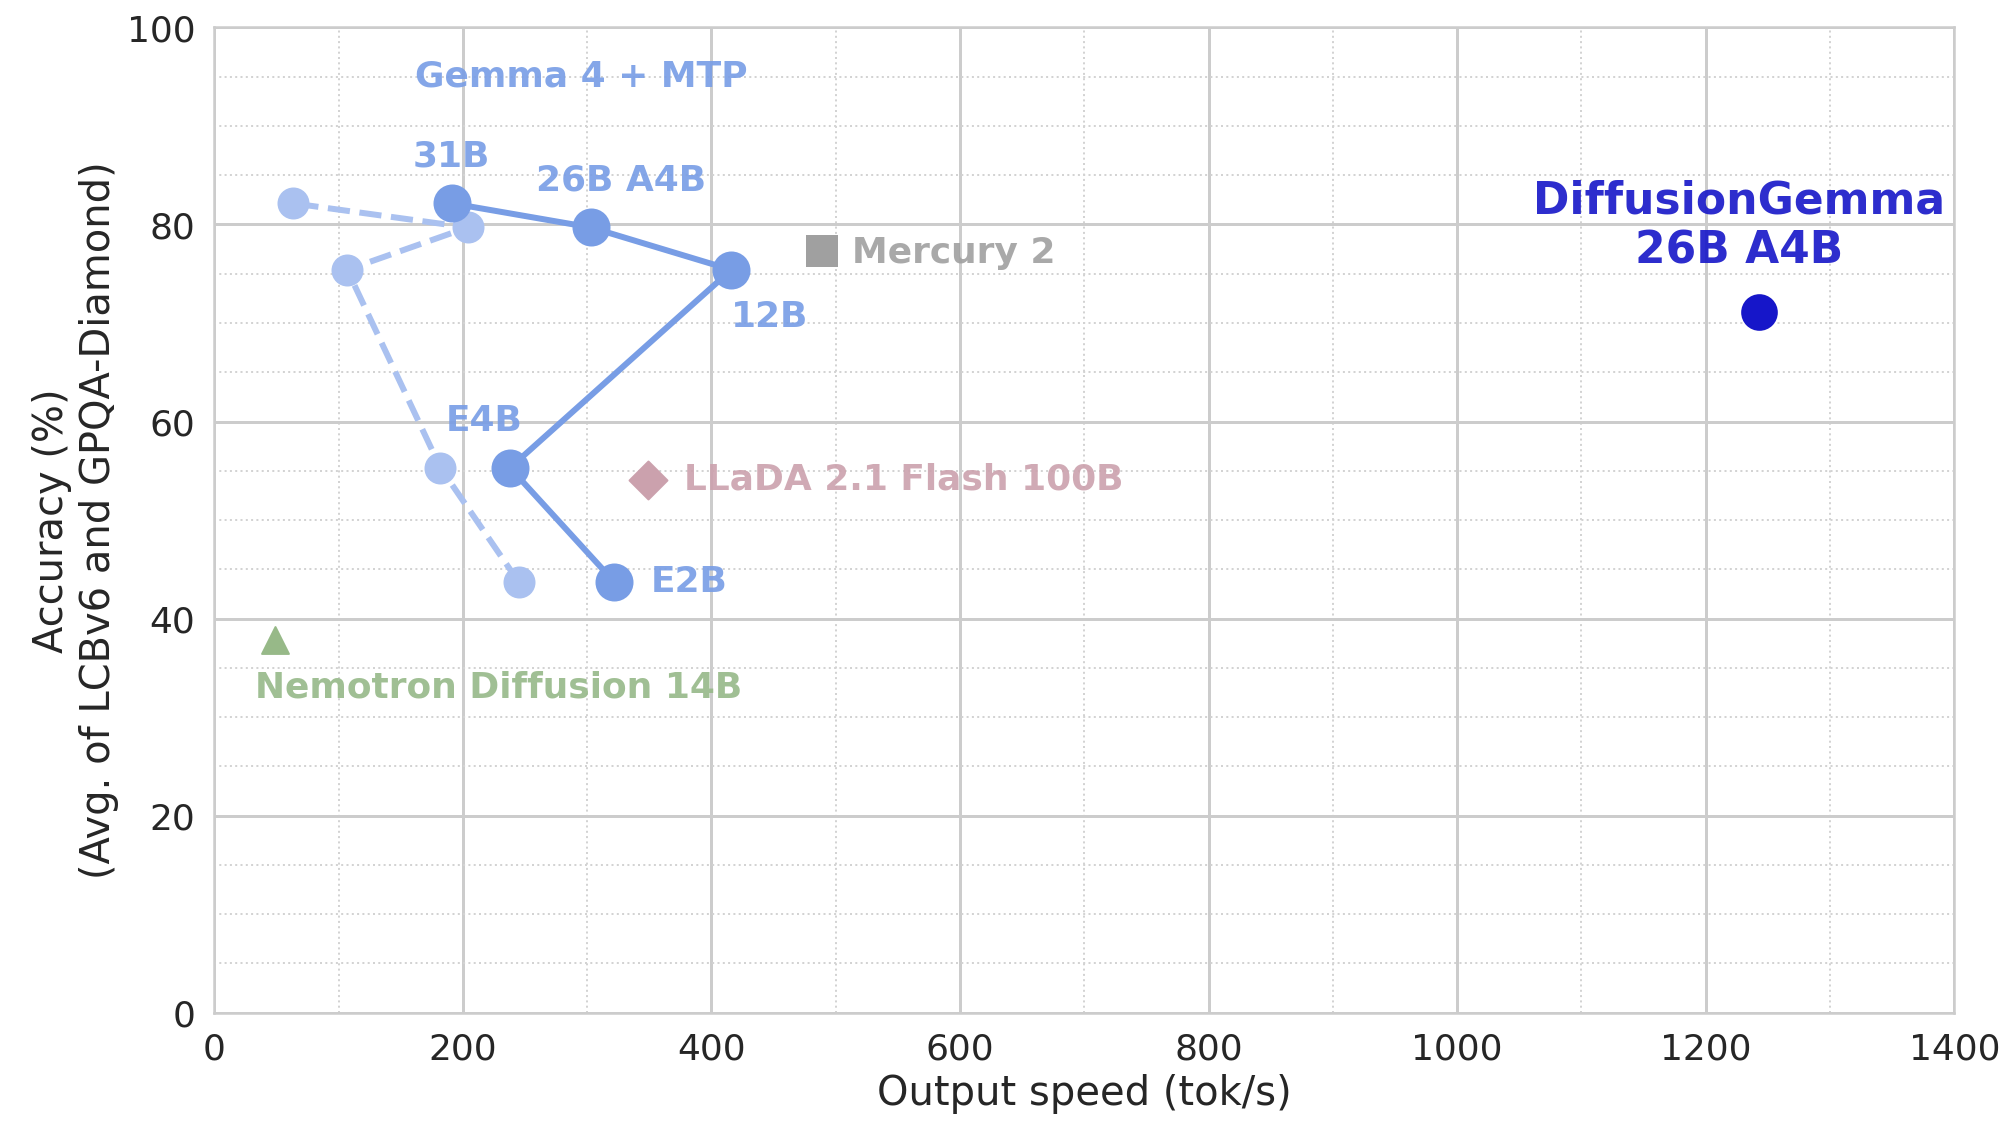
\includegraphics[width=0.85\linewidth, trim=0cm 0cm 0cm 0cm, clip]{assets/intro/pareto-plot-final4.png}
    \caption{\textbf{DiffusionGemma와 Gemma 4 계열 및 다른 diffusion 모델을 비교한 품질 대비 output decoding 속도 Pareto plot.} 품질과 output 속도는 모든 모델에 대해 GPQA-Diamond와 LiveCodeBench-v6 평균으로 계산했다. Gemma 4와 DiffusionGemma의 output 속도는 단일 H100(FP8, batch size~1)에서 측정했다.\textsuperscript{2} Nemotron~14B는 단일 H100(bfloat16, batch size~1), LLaDA~2.1 Flash~100B는 8$\times$ NVIDIA~B200 GPU(bfloat16, batch size~1)에서 측정했다.\textsuperscript{3} Mercury 2는 공개 OpenRouter API의 \texttt{high} reasoning effort 설정으로 측정했다(속도 추정은 Appendix~\ref{sec:competitor-eval-methodology} 참조). 연한 파란 점과 점선은 MTP가 \emph{없는} Gemma 4 모델 계열을 나타낸다.
    }
    \label{fig:final-pareto}
\end{figure}

\newpage

\section{소개}

Autoregressive (AR) 모델은 현재 Large Language Model (LLM) 환경을 지배하고 있지만, 엄격한 좌에서 우로의 token-by-token 생성 방식은 심각한 메모리 병목을 만든다. 많은 요청을 동시에 처리할 때는 batching으로 어느 정도의 처리량을 확보할 수 있지만, 단일 요청이나 동시성이 낮은 요청을 처리할 때는 본질적으로 memory-bound가 된다. 메모리에서 가속기로 모델 가중치와 context KV cache를 옮기는 데 걸리는 시간이 실제 연산 시간보다 훨씬 크기 때문이다. 이로 인해 가속기의 compute unit 활용률이 낮아지고 사용자당 생성 속도도 제한된다. speculative decoding은 작은 ``drafter'' 모델이 후보 시퀀스(보통 8 token)를 먼저 생성한 뒤, 이를 LLM에 넘겨 검증하게 함으로써 활용률을 높일 수 있다~\citep{leviathan2023fast,chen2023accelerating,xia-etal-2024-unlocking}. draft 길이가 8일 때는 forward pass당 3-6 token(TPF)을 생성할 수 있다~\citep{li2026eagle}. 그러나 이 draft-then-verify 패러다임에도 한계가 있다. 한편으로 AR drafter는 순차 생성 병목에 묶여 있고, 다른 한편으로 초기 blockwise decoding~\citep{stern2018blockwise}과 lookahead 전략~\citep{zhao2024lookahead}에 기반한 병렬 drafter는 뒤쪽 draft 위치로 갈수록 acceptance rate가 떨어진다~\citep{cheng2026dspark}.


Text diffusion은 token 전체 블록을 동시에 예측함으로써(Figure~\ref{fig:text_diffusion_sample}) 이 병목을 우회하며, 실행 특성을 memory-bound 영역에서 compute-bound 영역으로 사실상 이동시킨다. 최근에는 Gemini Diffusion \citep{deepmind2025geminidiffusion}, Mercury \citep{labs2025mercury}, LLaDA \citep{nie2026large,bie2025llada2}, Seed Diffusion \citep{song2025seed}, Nemotron-Labs-Diffusion \citep{fu2026nemotronlabsdiffusion} 등과 함께 text diffusion에 대한 관심이 급증하고 있다 \citep{deschenaux2024promises}. 그러나 현재 환경에서는 속도, 지능, 접근성 사이에서 뚜렷한 절충을 강요받는다. 예를 들어 Gemini Diffusion과 Mercury 같은 일부 모델은 proprietary API 뒤에 묶여 있다. 반대로 기존 open-weights 대안은 reasoning 능력과 multimodal 이해가 제한적이거나, diffusion 기술이 약속하는 극단적 저지연 이점을 충분히 제공하지 못하거나, 혹은 그 둘 모두에 해당한다. 지금까지 매우 높은 지능, 예외적으로 빠른 속도, 그리고 개방된 접근성을 동시에 갖춘 text diffusion 모델은 존재하지 않았다.



\begin{figure}[t!]
    \centering
    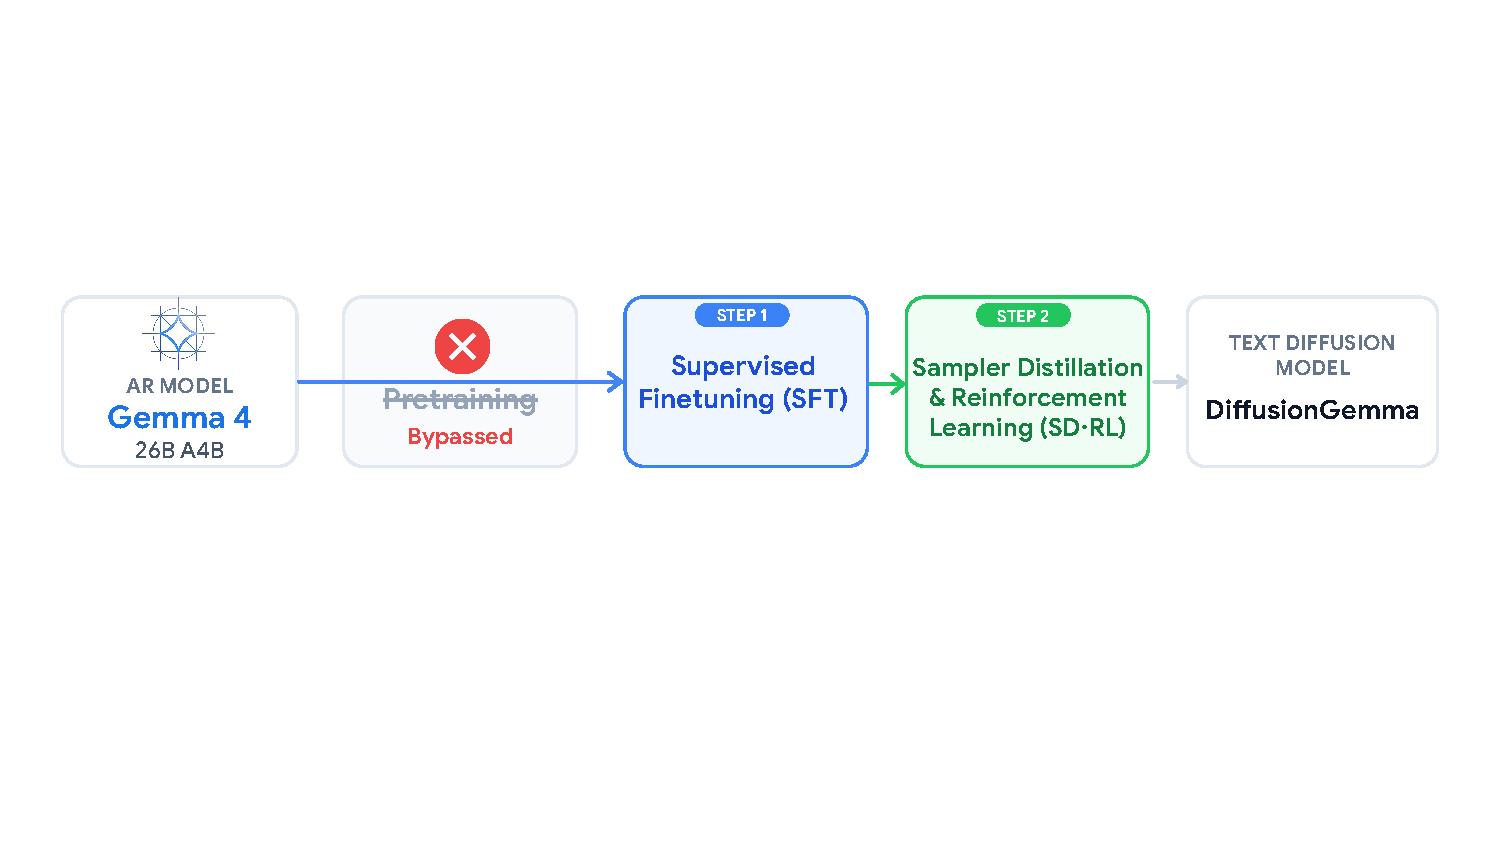
\includegraphics[width=1.0\linewidth,trim=0cm 6cm 0cm 4cm,clip]{assets/intro/diffusiongemma-recipe.pdf}
    \caption{\textbf{autoregressive 모델(Gemma 4 26B A4B)을 text diffusion 모델(DiffusionGemma)로 바꾸는 2단계 학습 파이프라인 개요.} AR 모델 가중치에서 초기화한 뒤, 모델은 먼저 discrete text diffusion과 256-token canvas 전반의 양방향 attention에 적응하는 SFT를 거친다. 이어서 온라인 sampler distillation 및 reinforcement learning 단계를 수행하며, 이는 보상 기반 생성 품질을 높이는 동시에 denoising step을 압축하여 초저지연을 달성한다.
    }
    \label{fig:recipe}
\end{figure}

우리는 이 격차를 메우기 위해 DiffusionGemma를 제안한다. Gemma~4 26B A4B mixture-of-experts (MoE)
모델 \citep{gemmateam2026gemma4technicalreport}을 text diffusion으로 finetuning한 변형인 이 모델은 생성 텍스트 모델링에서 지능과 속도 사이의 절충에 새로운 Pareto frontier를 제시한다(Figure~\ref{fig:final-pareto}). 특히 이 모델은 AR 모델에 최신 speculative decoding 기법인 multi-token prediction~\citep[MTP,][]{google2026mtpgemma4, deepseekai2024deepseekv3}을 장착한 경우에도, 모든 파라미터 규모(E2B에서 31B까지)에 걸쳐 기존 text diffusion 모델과 Gemma 4 AR 계열 모두보다 더 앞선 속도 frontier를 형성한다. 이 새로운 속도-지능 frontier를 열기 위해 DiffusionGemma는 약 12회의 forward pass에서 256 token 블록을 동시에 출력함으로써 알고리즘 효율을 극대화한다. 다시 말해 DiffusionGemma는 평균 20 TPF를 생성하는데, 이는 최신 speculative decoding 기법이 달성할 수 있는 약 3-6 TPF에 비해 도약적인 개선이다. 전체 forward pass 수가 크게 줄어들면서 diffusion 모델의 더 무거운 개별 forward pass 비용이 직접 상쇄되고, 그 결과 DiffusionGemma는 단일 NVIDIA H100 GPU에서 초당 약 1,500 token(TPS)의 생성 속도를 낸다. 또한 \citet{unsloth} 같은 제3자 inference 제공자의 초기 벤치마킹에 따르면 이 속도는 NVIDIA RTX 6000에서 최대 2,000 TPS까지 확장될 수 있다.



사전학습의 막대한 계산 비용을 피하기 위해, text diffusion 모델을 사전학습된 AR 모델에서 초기화하는 것은 일반적인 관행이다 \citep{han2024transfer,Gong2024ar2diff}. 우리는 DiffusionGemma를 Gemma 4 26B A4B MoE 모델의 최종 post-training 공개 가중치에서 warm-start한다~\citep{gemmateam2026gemma4technicalreport}. 같은 transformer backbone을 채택함으로써, AR 가중치를 효율적으로 재활용해 context encoding을 위한 causal attention과 diffusion 과정을 위한 bidirectional attention을 모두 지원하게 하면서도 기존 능력을 그대로 계승한다. 우리는 AR 모델 전체 학습 token의 10\% 미만만 사용하는 2단계 학습 파이프라인(Figure~\ref{fig:recipe})을 사용한다:

\begin{enumerate}[topsep=0pt]
    \item \textbf{Supervised fine-tuning (SFT)}: 먼저 SFT 단계를 수행해, 모델이 clean token으로 이루어진 context에 주의를 기울이는 동시에 256 noisy token 블록을 block 전반의 bidirectional attention으로 denoise하도록 적응시킨다(이는 diffusion 과정이 정하는 설정이다).
    \item \textbf{Sampler distillation and reinforcement learning (\sdrl)}: 이어서 생성 품질은 높이고(보상을 최대화하여), 초저지연은 확보하는( forward pass 수를 크게 줄여서) 온라인 학습 단계를 적용한다.
\end{enumerate}

AR 출발점의 특징을 유지함으로써, DiffusionGemma는 강한 multimodal 이해, long-context 능력, thinking mode를 보여 주며, 응답 전에 reasoning trace를 생성할 수 있다. 이는 현재 frontier 시스템의 대표적 특징이다 \citep{geminiteam2025gemini}. 모델을 diffusion 체계에 적응시키는 과정은 원래 AR baseline 대비 성능 손실을 유발하지만, inference 속도의 막대한 향상은 latency-critical 애플리케이션에 전혀 새로운 operating point를 제공한다. DiffusionGemma는 또한 autoregressive하게 텍스트를 생성하는 능력을 유지한다. 이러한 \textit{dual mode}는 지연 제약과 작업 복잡도에 따라 요청을 동적으로 라우팅하거나 hybrid decoding 접근을 사용할 가능성을 연다.



\begin{table}[t!]
\centering
\begin{minipage}[t]{0.43\textwidth}
\centering
\begin{tabular}[t]{ll}
\toprule
총계 & 25.2B \\
활성 & 3.85B \\
비전 인코더 & 550M \\
임베더 & 740M \\
Self-Conditioning & 7.8M \\
활성 / 전체 Expert 수 & 8 / 128 \\
 &  + 공유 1개 \\
\bottomrule
\end{tabular}
\caption{\textbf{파라미터 수.} DiffusionGemma 아키텍처는 262k token vocabulary를 갖는 mixture-of-experts transformer다. 총 활성 파라미터 수에는 vision encoder가 포함되지 않는다. self-conditioning을 위해 추가 MLP block도 포함된다.}
\label{tab:parameter-counts}
\end{minipage}\hfill
\begin{minipage}[t]{0.53\textwidth}
\centering
\begin{tabular}[t]{ll}
\toprule
Canvas 길이 & 256 \\
Sampler 최대 Denoising Step 수 & 48 \\
Adaptive Stopping Entropy 임곗값 & 0.005 \\
Token 선택 Entropy 임곗값 & 0.1 \\
Temperature 스케줄(선형) & 0.8 $\rightarrow$ 0.4 \\
\bottomrule
\end{tabular}
\caption{\textbf{Diffusion denoising 및 권장 sampler hyperparameter.} 실제로는 작업에 따라 adaptive stopping을 사용할 때 평균 sampler denoising step 수가 12이다.}
\label{tab:diffusion-hyperparams}
\end{minipage}
\end{table}

\paragraph{Open-weights 공개.} 우리는 최첨단 text diffusion 기술에 대한 접근을 넓히기 위해, Apache 2.0 라이선스 아래 DiffusionGemma를 open weights로 공개한다. 모델 파라미터에 대한 완전하고 제한 없는 접근을 제공함으로써, 연구자와 개발자, 실무자가 폭넓게 활용할 수 있는 생태계를 만들고자 한다. 연구 커뮤니티에는 discrete diffusion의 작동 원리를 깊이 있게 분석할 수 있는 강력한 white-box 기준선을 제공하고, 개발자에게는 제한 없는 사용 조건 아래 실험용 프로토타입과 상용 애플리케이션에 모두 쉽게 통합할 수 있는 기반을 제공한다.


중요하게도, DiffusionGemma의 매우 효율적인 아키텍처는 빠른 domain-specific 적응을 위한 이상적인 기반이 된다. 계산 진입 장벽을 크게 낮춤으로써, 커뮤니티는 제한된 compute 예산 환경에서도 각자의 고유한 사용 사례에 맞는 초고속 task-specific 모델을 손쉽게 finetune할 수 있다. 이러한 가볍고 빠른 반복 가능성은 즉각적인 커뮤니티 채택을 촉진했다. 집필 시점 기준으로 모델이 공개된 지 몇 주밖에 되지 않았음에도, 이미 특화된 downstream 애플리케이션의 엔진으로 사용되고 있다. 이렇게 빠르게 등장하는 활용 사례는 다국어 automatic speech recognition~\citep{interfaze2026diffusion}부터 의료 분야의 대화형 radiology report 초안 작성~\citep{van2026discrete}까지, 매우 다양하고 까다로운 영역에 걸친 모델의 범용성을 보여 준다.

\paragraph{개요.}
이 기술 보고서의 나머지 구성은 다음과 같다. Section~\ref{sec:background}에서는 discrete diffusion 프레임워크와 우리의 접근을 뒷받침하는 이론적 토대를 정식화한다. Section~\ref{sec:architecture}에서는 bidirectional decoding 메커니즘과 sampling 알고리즘을 포함한 DiffusionGemma 아키텍처를 자세히 설명한다. 이어서 학습 파이프라인의 두 단계를 다룬다. 먼저 Section~\ref{sec:sft}의 SFT 단계, 그다음 sampler distillation과 reinforcement learning을 결합한 온라인 학습 단계인 Section~\ref{sec:sdrl}이다. Section~\ref{sec:inference_optimizations}에서는 저수준 inference 최적화를 해부하고, Section~\ref{sec:experiments}에서는 실험 결과를 제시한다. Section~\ref{sec:downstream_sft}에서는 downstream 애플리케이션을 위한 DiffusionGemma finetuning 방법과 실용적 예시를 제공한다. Section~\ref{sec:advantages}에서는 text diffusion의 실질적 장점을 보여 주고, 마지막으로 Section~\ref{sec:limitations}에서 한계와 알려진 이슈를 논의한 뒤 Section~\ref{sec:conclusion}에서 결론을 맺는다.



\section{Discrete Diffusion을 이용한 생성 텍스트 모델링} \label{sec:background}

역사적으로 LLM은 텍스트 생성을 엄격한 순차 과정으로 다루어 왔다~\citep{bengio2003neural, mikolov2010recurrent, graves2013generating, sutskever2014sequence, Vaswani2017, gu2018nonautoregressive}. 고전적인 AR language modeling은 길이 $L$인 시퀀스 $x$의 결합확률을 조건부 확률의 정확한 곱으로 분해한다: $p(x) = \prod_{i=1}^L p(x^i \mid x^{<i})$. 여기서 $i$는 시퀀스 내 token 위치를 나타낸다. 이 방식은 이론적으로는 엄밀하지만, 심각한 memory-bandwidth 제약 때문에 현대 하드웨어 가속기에서 생성 속도를 본질적으로 제한하며, 동시에 미래 token을 바탕으로 token을 양방향으로 수정하는 것도 엄격하게 막는다~\citep{leviathan2023fast, savinov2022sundae}.

Diffusion 모델은 결합분포 $p(x)$를 엄격한 좌에서 우로의 위치가 아니라 noise level의 연속(즉 Markov chain) 위에서 생성 과정을 분해함으로써 근사한다~\citep{sohl2015deep, ho2020denoising, song2020score, holderrieth2025}. 이는 score-matching과 continuous-time flow model에 관한 기초 연구 위에 세워진다~\citep{song2019generative, song2021denoising, song2021maximum, meng2022sdedit, lipman2023flow, debortoli2021diffusion}. 학습 시에는 순방향 과정이 clean data를 점진적으로 random noise로 오염시키고, 신경망은 그 역방향 denoising 과정을 학습하도록 훈련된다. inference 시에는 random noise에서 시작해 출력 시퀀스를 병렬로 반복 정제함으로써 전체 데이터 시퀀스를 생성한다.


Diffusion을 텍스트에 적용하려면 언어의 discrete한 성질을 다뤄야 한다~\citep{yi2024diffusion}. 초기 접근들은 discrete token을 연속 embedding 공간으로 사상함으로써 표준 Gaussian diffusion을 텍스트에 적용했다. 이들 모델은 텍스트로 되돌리는 방식에서 주로 차이가 난다. Diffusion-LM \citep{li2022diffusionlm}이나 SED \citep{strudel2022self} 같은 아키텍처는 강제로 투영하거나 ``반올림''해서 discrete token으로 되돌려야 하는 연속 벡터를 생성하는 반면, CDCD \citep{dieleman2022continuous} 같은 방법은 연속 과정을 유지하면서도 categorical logits를 직접 예측해 token을 sampling한다. 디코딩 방식과 무관하게, 이런 정식화는 이론적·기하학적 도전에 직면하며, 결국 native discrete diffusion 모델에 비해 효과가 제한된다. 특히 hard rounding 연산은 continuous-time 및 variational 정식화가 제공하는 diffusion likelihood bound의 정확성을 근본적으로 깨뜨리고 \citep{kingma2021variational}, 유효한 vocabulary token은 고차원 latent 공간에서 극히 작은 비율만 차지한다. 그 결과 역생성 과정은 종종 공간의 비어 있고 ``무의미한'' 영역으로 표류하며, 이를 가장 가까운 token으로 반올림하면 퇴화된 embedding이 임의의 무관한 token으로 매핑되어 비일관적 텍스트를 만들어 낸다 \citep{shabalin2025tencdm, meshchaninov2025cosmos}. 이러한 공간적 표류를 막기 위해 step별 discretization 메커니즘에 의존하는 방법들이 개발되었지만, 대개 연속 공간을 충분히 활용하지 못하고 생성 유연성도 제한한다 \citep{hu2026elf}.

Discrete diffusion은 매우 효과적인 대안으로 부상했다 \citep{austin2021structured, sahoo2024simple, lou2024discrete, zhao2024unified}. 이 패러다임은 초기 bidirectional 모델의 single-step corruption heuristic을 정식적인 multi-step Markov process로 일반화한다. absorbing mask state나 vocabulary 전반의 multinomial 분포처럼 현대 diffusion에서 categorical state 사이에 정의되는 확률적 전이는, BERT가 도입한 masking과 random token swapping \citep{devlin2019bert, liu2019roberta, sanh2019distilbert}, 그리고 ELECTRA의 그럴듯한 token replacement \citep{clark2020electra}의 직접적인 후손이다. continuous vector가 아니라 discrete state 위에서 직접 작동함으로써, discrete diffusion은 embedding projection 불일치를 완전히 피하고 categorical transition에 대해 더 나은 이론적 기반을 제공한다 \citep{gat2024discrete}. DiffusionGemma는 이러한 discrete diffusion 계보를 바탕으로 높은 충실도의 token 생성을 보장한다.


\subsection{확률 경로와 Denoising}

우리의 discrete diffusion 프레임워크를 정식화하기 위해, 최근 문헌에서 확립된 continuous-time Markov chain (CTMC) 접근을 채택한다 \citep{campbell2022continuous, campbell2024generative, gat2024discrete}. $\Vcal$을 크기 $V$의 categorical token vocabulary라고 하자. 반복 정제를 거치는 token 시퀀스를 우리는 길이 $C$의 \emph{canvas}라고 부른다. 시간 $t \in [0, 1]$에서 이 canvas의 한 실현은 벡터 $x_t \in \Vcal^C$로 나타낸다. 우리는 시간 $t=0$의 clean data 분포 $p$와 시간 $t=1$의 완전히 오염된 source canvas 사이를 부드럽게 보간하는 marginal probability path를 구성한다. 이 경로의 시작에서 clean token은 $x_0 \sim p(\cdot)$로 정의되며, 이는 궁극적으로 완전히 오염된 상태 $x_1 \sim \unif(\Vcal^C)$로 전이한다. 여기서 $\unif(\Vcal^C)$는 결합 상태 공간에 대한 uniform prior를 뜻하며, $C$개의 각 token이 $\Vcal$ 위에서 서로 독립적으로 균등분포를 따른다. 이 corruption 과정은 order-agnostic discrete diffusion 모델에서 흔히 사용되는 uniform noise나 absorbing masking 같은 명시적 전이 행렬과 상응한다 \citep{hoogeboom2022autoregressive}. 연속 시간에서 작동하기 때문에, 이 프레임워크는 전통적인 AR 모델의 순차적 좌에서 우로의 디코딩 병목을 우회하며, 전체 canvas의 token을 병렬로 처리하고 정제할 수 있게 한다.

\begin{figure*}[!t]
    \centering
    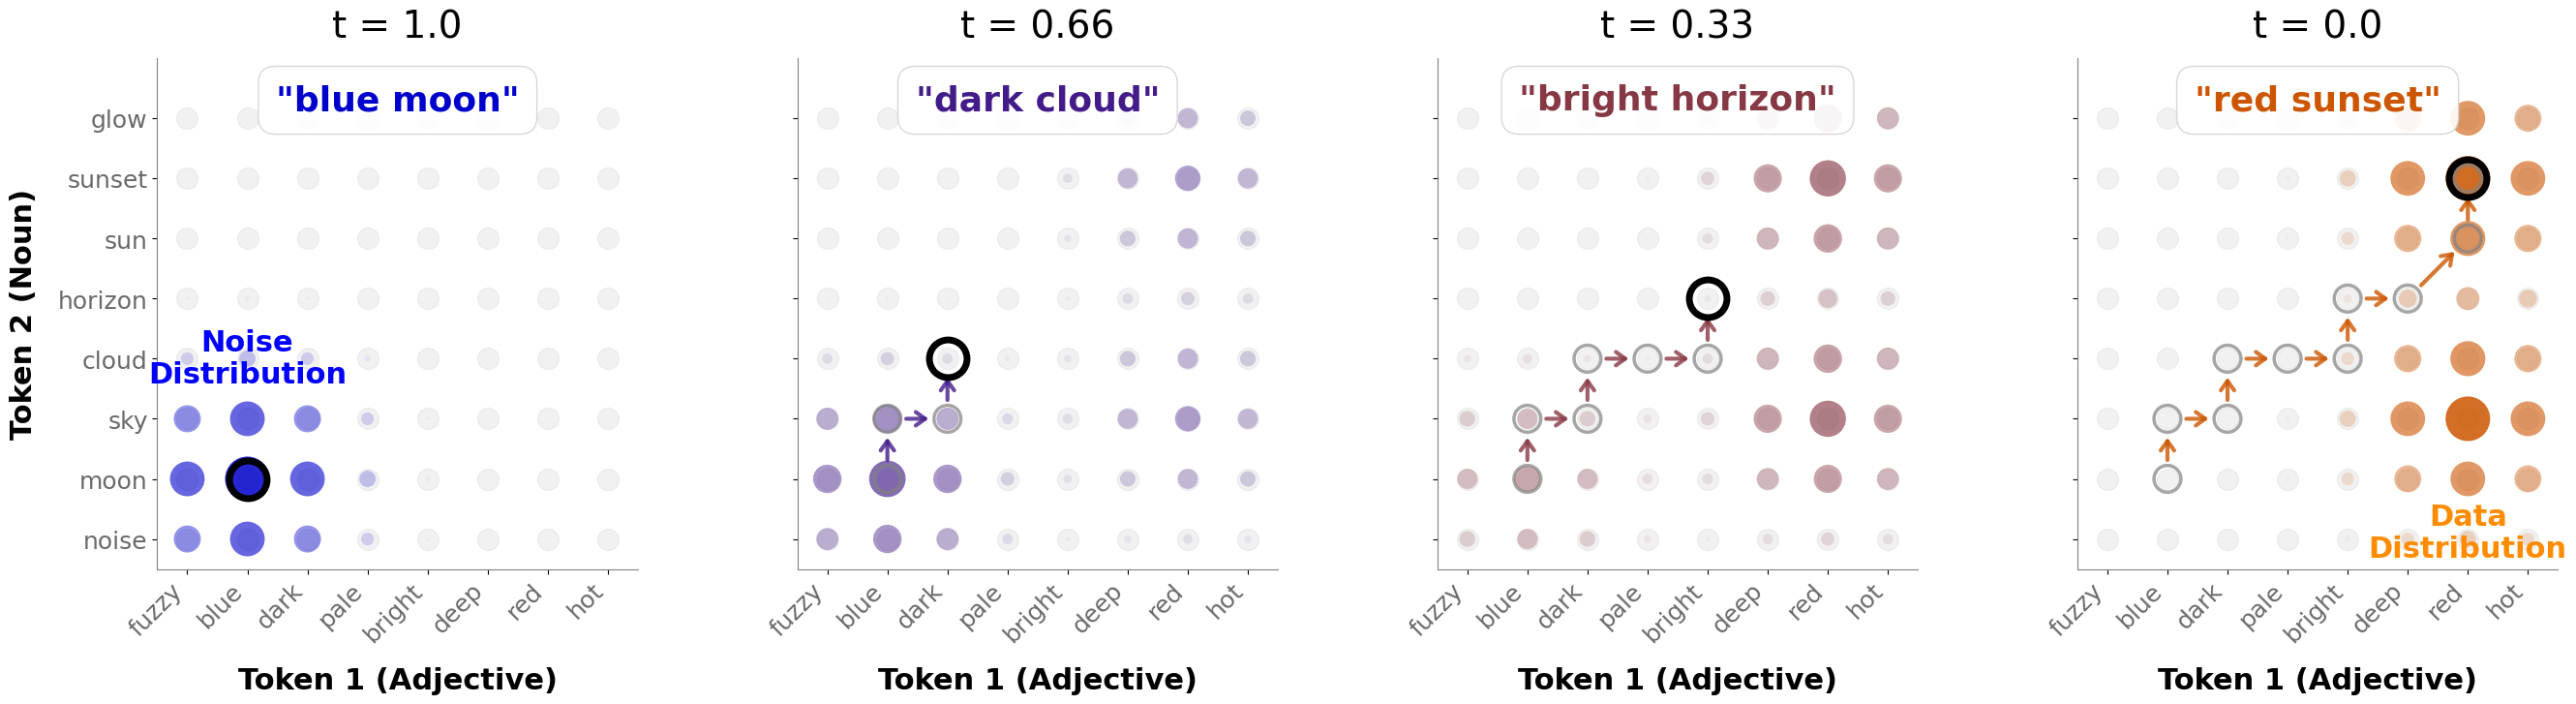
\includegraphics[width=1.0\linewidth]{assets/discrete_diff_figures/discrete_diff_illustration.png}
    \caption{\textbf{discrete diffusion 확률 경로와 병렬 sampling trajectory의 예시적 그림.} 설명을 위해 상태 공간은 token마다 다른 vocabulary를 사용한다. 가로축은 형용사, 세로축은 명사다. 시간이 $t = 1.0$(noise)에서 $t = 0.0$(data)로 거꾸로 흐를수록, 주변 분포는 균일한 noise 분포에서 벗어나 유효한 data mode로 확률 질량을 집중시키며 부드럽게 보간된다. 검은 원은 개별 시퀀스 실현의 discrete jump transition을 추적하며($t=1.0$의 ``blue moon''에서 $t=0.0$의 ``red sunset''까지), 병렬 canvas 차원이 시간이 흐르며 non-autoregressive하게 조정되는 방식을 보여준다.}
    \label{fig:discrete_diff}
\end{figure*}

\subsubsection{순방향 과정}
순방향 과정은 clean 텍스트 token이 균등분포 token으로 전이되는 방식을 규정한다. 고정된 clean 시작 canvas $x_0$가 주어졌을 때, 순방향 전이 확률 경로는 각 token 좌표 $i$에 대해 독립적으로 분해된다:
\begin{equation}\label{eq:factorized_path_pmf}
    \mathbb{P}(X_t=x_t \mid X_0 = x_0) =
    \prod_{i=1}^C \left[ \kappa_t \delta(x_t^i, x_0^i) + (1 - \kappa_t) \frac{1}{V} \right],
\end{equation}
여기서 $\kappa_t \in [0,1]$는 $\kappa_0 = 1$에서 $\kappa_1 = 0$으로 부드럽게 감소하는 noise schedule이며, $\delta$는 Kronecker delta를 나타낸다. 실질적으로는 시간 $t$가 $1$을 향해 갈수록 각 token이 vocabulary에서 균등무작위로 뽑힌 token으로 대체될 확률이 점점 커진다 \citep{hoogeboom2021argmax, austin2021structured}. 우리는 이 closed-form 순방향 과정을 사용해 clean 텍스트로부터 학습 데이터를 생성한다.

\subsubsection{역방향 Denoising 과정}
Noise로부터 데이터를 복원하기 위해, 우리는 이 categorical corruption을 되돌리는 역과정을 학습한다. discrete flow matching 이론에 따르면 순방향 trajectory를 완벽히 되돌리려면, 오염된 상태가 주어졌을 때 원래의 clean token 조건부분포를 추론해야 한다 \citep{campbell2024generative, gat2024discrete, ou2025absorbing}. 주어진 실현 $X_t = x_t$에 대해, 시간축을 작은 간격 $\Delta t$만큼 뒤로 이동하는 과정은 어떤 전이 mapping에 의해 지배되며, 이를 우리는 $\step$으로 표기한다. 이 함수는 다음 중간 step에 대한 확률분포를 출력한다\footnote{전형적인 예로, 함수 $\step$은 \citet{gat2024discrete}에서 도입된 discrete Euler update step으로 구현할 수 있다. 이때 $
\mathbb{P}(X_{t-\Delta t}^i = v \mid X_t = x_t) \approx \delta(v, x_t^i) - \Delta t \frac{\dot{\kappa}_t}{1 - \kappa_t} \left[ \mathbb{P}(X_0^i = v \mid X_t = x_t) - \delta(v, x_t^i) \right]$ with $\kappa_t \in [0, 1]$.}:
\begin{equation}\label{eq:transition-mapping}
\mathbb{P}(X_{t-\Delta t} = \cdot \mid X_t = x_t) \approx \operatorname{Step}\Big(x_t, \mathbb{P}(X_{0} = \cdot \mid X_t = x_t)\Big).
\end{equation}
이 업데이트를 계산하려면 noisy state가 주어졌을 때 clean token의 진짜 posterior 분포 $\mathbb{P}(X_{0}^i = v \mid X_t = x_t)$가 필요하다. 우리는 이 posterior를 신경망 $p_\theta(v \mid x_t)$로 근사한다. 생성 시에는 이 근사를 사용해 다음 token state를 sampling한다: $x_{t-\Delta t} \sim \operatorname{Step}(x_t, p_\theta(\cdot \mid x_t))$.

Figure \ref{fig:discrete_diff}는 이 역방향 sampling trajectory를 단순화된 2-token canvas($C=2$) 안에서 설명하기 위한 매우 도식적인 예시를 보여 준다. 시간이 $t=1.0$에서 $t=0.0$으로 거꾸로 흐르면서, 모델은 균일한 noise 분포(예: ``blue moon'' 부근)에서 확률 질량을 부드럽게 빼내 유효한 data mode로 옮긴다. 동시에 개별 시퀀스 좌표는 연속시간 jump transition을 겪는데, 이는 $t=1.0$의 ``blue moon''에서 $t=0.66$의 ``dark cloud''를 거쳐 최종적으로 $t=0.0$의 ``red sunset'' 같은 고확률 mode에 도달하는 단계별 경로로 시각화된다. 이는 순차적 좌에서 우로의 생성 없이도 병렬 차원들이 시간에 따라 어떻게 조정되는지를 보여 준다.

이 denoising 과정은 factorized되어 있으므로, 개별 역방향 step 동안 조건부 독립성을 가정한다. 위치 $i$에서 새로 업데이트되는 token은 현재 noisy canvas~$x_t$ 전체를 조건으로 삼지만, 다른 위치들($j \neq i$)에서 동시에 이루어지는 sampling 선택은 볼 수 없다. 이러한 구조적 절충은 때때로 국소적 불일치나 상충하는 문법 예측을 유발할 수 있다. 다음 절에서는 이러한 비조정적 메커니즘을 우리의 \emph{self-conditioning architecture}와 \emph{entropy-bounded sampling} 전략으로 직접 보완한다.


\section{DiffusionGemma 아키텍처} \label{sec:architecture}

DiffusionGemma 아키텍처는 \emph{shared weights}~$\theta$를 갖는 encoder-decoder transformer \citep{Vaswani2017}로 작동한다. diffusion 모델을 처음부터 사전학습하는 대신, 우리는 공개된 Gemma 4 26B A4B MoE checkpoint~\citep{gemmateam2026gemma4technicalreport}로 모델을 초기화한다. 기존 AR backbone에 아키텍처를 묶는 것은 절대적인 생성 품질 일부를 양보하는 대신 학습 계산 비용을 크게 줄이는 실용적 선택이다. 또한 이 초기화 덕분에 확장된 context window와 native multimodal 이해 같은 기반 모델의 고급 기능도 계승할 수 있다. 더 나아가 우리의 실험은 최종 모델 가중치가 autoregressive sampling 능력도 유지함을 보여 준다(표~\ref{tab:model_comparison} 참조).

이 절의 나머지에서는 DiffusionGemma가 inference 시 이 아키텍처를 사용해 어떻게 텍스트를 생성하는지 자세히 설명한다. 우리는 이 과정을 세 요소로 나누어 다룬다. 긴 시퀀스를 처리하기 위한 block-autoregressive decoding 전략(Section~\ref{sec:block-ar}), 개별 canvas denoising을 위한 일반 프레임워크(Section~\ref{sec:denoising}), 그리고 구체적인 entropy-bounded sampler(Section~\ref{sec:sampling})이다.

\begin{figure}[t!]
    \centering
    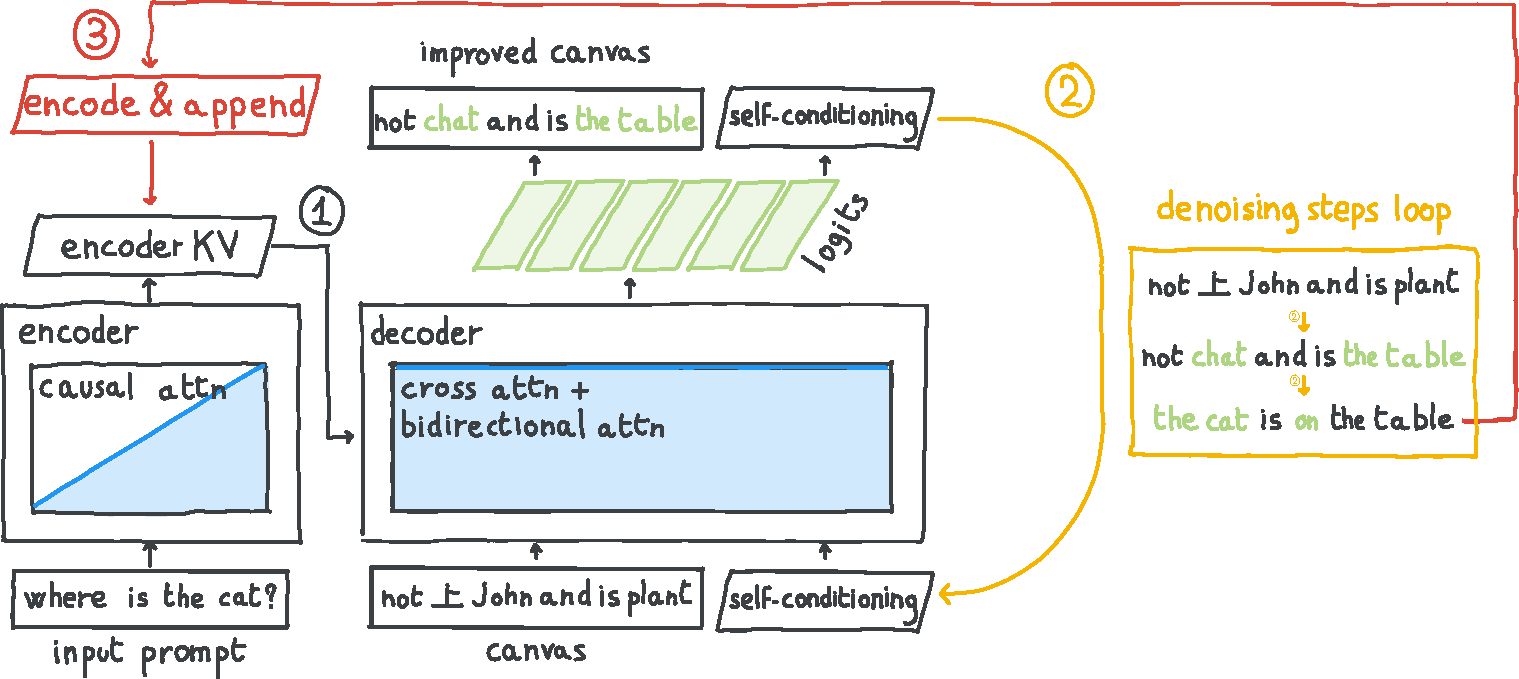
\includegraphics[width=0.9\textwidth]{assets/encoder-decoder-rev-d.pdf}
    \caption{\textbf{DiffusionGemma 생성 파이프라인.} 이 과정은 세 단계로 이루어진다. 1) \textbf{Context encoding:} 입력 prompt를 causal encoder가 처리해 Key-Value (KV) cache를 초기화한다. 2) \textbf{Denoising loop:} noisy canvas를 decoder가 반복적으로 정제하며, canvas 전반의 양방향 attention과 KV cache에 대한 cross-attention을 사용해 텍스트를 완전히 denoise한다. 3) \textbf{Encode \& append:} 완성된 clean canvas를 다시 causal encoder에 통과시켜 KV cache에 추가하고, 다음 token block의 context를 설정한다.}
    \label{fig:encoder-decoder}
\end{figure}

\subsection{Block-Autoregressive 생성}\label{sec:block-ar}

Section~\ref{sec:background}에서 소개한 discrete flow matching 정식화는 고정 길이 시퀀스에서 작동한다. open-ended 텍스트를 생성하기 위해 우리는 block-AR 생성 전략을 사용한다. 모델은 한 번에 256 token canvas를 denoise하고, 하나의 canvas가 완전히 denoise되면 이를 시퀀스 히스토리에 확정한 뒤 다음 canvas의 denoising을 시작한다.

\paragraph{KV cache 초기화.} Figure~\ref{fig:encoder-decoder}에 나타난 것처럼, block-AR 생성의 첫 단계는 context $h \in \Vcal^L$를 KV cache $H$로 인코딩하는 것이다. context에는 최대 token 수 $L$의 system instruction과 user prompt가 포함된다.\footnote{실제로 $h$에는 token vocabulary에 속하지 않는 interleaved multimedia embedding도 포함된다.} 이를 다음과 같이 쓴다
\begin{equation}
    \label{eq:encoder}
    H = \enc(h),
\end{equation}
여기서 $\enc$는 가중치 $\theta$와 causal attention mask를 사용하는 transformer forward pass다.

\paragraph{KV cache 조건부 Canvas denoising.} KV cache $H$에 cross-attention함으로써, canvas 생성은 system instruction, user input, 과거 응답에 조건부가 될 수 있다. canvas 생성은 균등무작위 token으로 이루어진 canvas에서 시작하며, Sections~\ref{sec:denoising}과~\ref{sec:sampling}에서 설명한 과정을 사용해 반복적으로 denoise된다. canvas가 완전히 denoise되면,\footnote{canvas는 $t=0$에 도달하거나 Section~\ref{sec:sampling}에서 설명한 adaptive stopping 조건을 만족할 때 완전히 denoise된 것으로 본다.} 이를 $\hat{x}_0$로 표기하고, 그 key와 value를 KV cache에 추가한다(Figure~\ref{fig:encoder-decoder}의 빨간색 부분):
\begin{equation}
    \label{eq:updated_kv_cache}
    H \gets H \oplus \enc(\hat{x}_0).
\end{equation}
이 denoising 과정은 모델이 자신의 턴 종료를 나타내는 special token을 생성할 때까지 이후 canvas들에 대해 반복되며, 그 뒤 모든 canvas $\hat{x}_0$를 이어 붙여 최종 응답을 만든다. encoder에서 causal attention을 사용하기 때문에, encoder는 가장 최신 canvas만 덧붙여 KV cache를 갱신할 수 있다. 이는 BART \citep{lewis2020bart}나 T5 \citep{raffel2020exploring} 같은 표준 encoder-decoder 모델을 구조적으로 뒤집은 형태다. 기존 모델이 context에는 bidirectional encoder를, 생성에는 causal decoder를 사용하는 반면, 우리의 접근은 시퀀스 히스토리에는 causal encoder를, diffusion 기반 canvas 생성에는 bidirectional decoder를 사용한다. 이런 causal encoding은 초기 context token이 최신 canvas를 보지 못하게 하지만, 증가하는 context 전체를 매번 처음부터 다시 인코딩할 필요를 없애므로 긴 reasoning 생성에도 확장 가능하며 diffusion과 AR 생성을 구조적으로 결합한다. 이 block-AR 전략은 우리 그룹이 2023년 6월의 미공개 원고에서 개발했으며, blockwise sequence modeling과 KV caching에 대한 유사한 접근은~\citet{wu2025fastdllmv2}, \citet{arriola2025block}, \citet{deschenaux2026blockgen}에 의해 독립적으로도 개발되었다.


\subsection{Inference 시 Denoising 프레임워크}\label{sec:denoising}

\paragraph{Canvas 초기화.} canvas를 생성하기 위해, 우리는 최대 $N$개의 denoising step에 걸쳐 step 크기 $\Delta t = 1 / N$로 이를 반복 정제한다. $x_t \in \Vcal^C$를 step $t$에서의 corrupted canvas라고 하자. 우리는 $t=1$에서 vocabulary $\Vcal$에서 균등무작위로 뽑은 token으로 이루어진 canvas $x_1$로 과정을 초기화한다.

\paragraph{Decoder forward pass.} 각 step $t$에서 우리는 shared weights $\theta$를 갖는 transformer를 decoder, 즉 $\dec$로 사용하여 clean token의 확률분포를 예측한다. decoder는 세 가지 입력을 받는다. 현재 noisy canvas $x_t$, context KV cache $H$, 그리고 모델의 이전 예측을 다시 자기 자신에게 되먹이는 연속 \textit{self-conditioning} 신호 $z_t \in \mathbb{R}^{C \times d}$이다 \citep{chen2023analog, strudel2022self, jo2026loopholing}. canvas token 전반의 bidirectional attention과 KV cache에 대한 cross-attention을 사용해, decoder는 정규화되지 않은 logits $L_t$를 출력한다:
\begin{equation} \label{eq:denoising-forward-pass}
    L_t = \dec(x_t, z_t, H) \in \mathbb{R}^{C \times V}.
\end{equation}

\paragraph{Denoising 반복.} 각 반복에서 우리는 logits $L_t$를 계산하고 clean token 확률 $\hat{p}_0$를 평가한 뒤, 다음 step을 위한 self-conditioning 신호를 갱신하고 정제된 canvas를 sampling한다:
\begin{equation} \label{eq:denoising-iteration}
\begin{aligned} 
    \hat{p}_0 &= \softmax \big(L_t/\tau_t\big) \in [0, 1]^{C \times V}, \\
    z_{t-\Delta t} &= \operatorname{FFW}(\hat{p}_0 E) \in \mathbb{R}^{C \times d},
    \\
    x_{t-\Delta t} &\sim \operatorname{Step}(x_t, \hat{p}_0).
\end{aligned}
\end{equation}
여기서 $E \in \mathbb{R}^{V \times d}$는 token embedding matrix이고 $\operatorname{FFW}$는 표준 feedforward network다. 시간 의존적인 temperature $\tau_t > 0$는 최종 전이 확률을 계산하기 전에 모델의 예측을 더 날카롭게 만들 수 있다. Equation~\eqref{eq:transition-mapping}에서 설명한 전이 mapping $\step$은 업데이트된 canvas $x_{t-\Delta t}  \in \Vcal^C$를 sampling하는 데 쓰일 categorical 분포를 계산하며, 이는 새로운 self-conditioning 신호 $z_{t-\Delta t}$와 함께 다음 denoising step으로 입력된다.
Section~\ref{sec:sampling}에서는 전이 mapping $\step$과 temperature $\tau_t$에 대한 우리의 구체적 선택을 설명한다.


\paragraph{Multinomial diffusion.} 우리의 denoising 반복(Equation~\ref{eq:denoising-iteration})은 masked diffusion이 아니라 multinomial(또는 uniform) diffusion을 사용한다 \citep{hoogeboom2021argmax, austin2021structured}. 모든 token이 서로 전이할 수 있기 때문에, 모델은 자신의 오류를 지속적으로 수정할 수 있다. 현재 canvas 안에서는 더 이른 denoising step($t' > t$)에서 받아들여진 token도 여전히 수정 가능하다. 다만 이전에 생성된 canvas의 token은 영구적으로 고정된다는 점을 밝힌다.

\paragraph{해석 가능성에 대한 주석.} 최근 interpretability 분석은 self-conditioning 신호 $z_t$가 시퀀스에 연속 latent space 주입을 도입함에도, 이러한 중간 self-conditioning 벡터가 해석 가능한 token bottleneck에 안정적으로 매핑되어 모델의 알고리즘적 투명성을 보존함을 보여 준다~\citep{engels2026how, asaria2026neither}.


\subsection{DiffusionGemma Sampler}
\label{sec:sampling}

temperature, top-$p$, top-$k$ 같은 경직된 heuristic에 의존하는 AR 생성과 달리, diffusion modeling은 discrete predictor-corrector 메커니즘과 multi-step solver를 포함하는 훨씬 더 풍부한 sampling 설계 공간을 도입한다 \citep{lezama2023predictor, deschenaux2026diffusion, liu2026nisampling, yao2026accelerating, ren2025fast}. 텍스트 생성을 반복적 시간 과정으로 바라보면 inference 시 알고리즘을 기반 아키텍처와 분리할 수 있어, 계산 비용과 생성 품질 사이의 절충을 세밀하게 제어할 수 있다.

Section~\ref{sec:denoising}에서 canvas denoising의 전체 접근을 설명했지만, 이 소절에서는 그 구체적 구현 하나를 다룬다. temperature annealing과 adaptive stopping을 결합한 entropy-bounded sampler \citep{ben2026accelerated}(Algorithm~\ref{alg:sampling})이다. 이것이 기본값이자 권장 sampler이긴 하지만, DiffusionGemma는 모듈식이므로 고품질 inference를 위해 반드시 이 정확한 sampling 설정에만 묶여 있지는 않다.

\begin{algorithm}[t!]
\caption{Entropy-Bounded Denoising과
Adaptive Stopping을 사용하는 DiffusionGemma Sampling}
\label{alg:sampling}
\small
\begin{algorithmic}[1]
    \Require Context $h$; 최대 denoising step 수 $N=48$
    \Require Entropy budget $b=0.1$;
         stopping 임곗값 $e_{\mathrm{stop}}=0.005$
    \Require Temperature 스케줄의 양 끝값
         $\tau_{\max}=0.8$ 및 $\tau_{\min}=0.4$

    \Statex \textbf{초기화}
\State $H \gets \enc(h)$
        \Comment{Causal-attention KV cache}
\State $\Delta t \gets 1/N$
\State $x_1 \sim \unif(\Vcal^C)$,
    \quad $z_1 \gets \boldsymbol{0}$
\State $\hat{x}_0^{\mathrm{prev}} \gets \bot$

    \Statex \textbf{Denoising}
\For{$n=1,\ldots,N$}
    \State $t \gets 1-(n-1)\Delta t$

    \State $L_t \gets \dec(x_t,z_t,H)$,
        \quad $L_t\in\mathbb{R}^{C\times V}$
    \State $\hat{x}_{0\mid t} \gets \arg\max(L_t)$
            \Comment{현재의 결정론적 예측}

    \State $\tau_t \gets
        (\tau_{\max}-\tau_{\min})t+\tau_{\min}$
    \State $\hat{p}_0 \gets
        \softmax(L_t/\tau_t)$

    \State $e^i \gets
        \operatorname{Entropy}(\hat{p}_0^i)$
        for all $i\in\{1,\ldots,C\}$
    \State $\bar{e} \gets
        \dfrac{1}{C}\sum_{i=1}^{C}e^i$

    \If{$n>1
        \land \bar{e}\leq e_{\mathrm{stop}}
        \land \hat{x}_{0\mid t}=\hat{x}_0^{\mathrm{prev}}$}
        \State \Return $\hat{x}_{0\mid t}$
            \Comment{Adaptive stopping}
    \EndIf

    \State $\hat{x}_0^{\mathrm{prev}}
        \gets \hat{x}_{0\mid t}$

    \If{$n<N$}
        \State $z_{t-\Delta t} \gets
            \operatorname{FFW}(\hat{p}_0E)$
            \Comment{$E$는 embedding matrix}

        \State $x_D \sim \hat{p}_0$

        \State Let $(\pi_1,\ldots,\pi_C)$ order positions
            by non-decreasing entropy
            \Comment{동률은 위치 인덱스로 해소}
        \Statex \hspace{\algorithmicindent}
            $e^{\pi_1}\leq e^{\pi_2}\leq\cdots\leq e^{\pi_C}$

        \State $k \gets
            \displaystyle\max\left\{
                m\in\{1,\ldots,C\}:
                \sum_{j=1}^{m-1}e^{\pi_j}\leq b
            \right\}$
        \State $U \gets \{\pi_1,\ldots,\pi_k\}$

        \State For each $i\in\{1,\ldots,C\}$, set
        \Statex \hspace{\algorithmicindent}
            $\displaystyle
            x_{t-\Delta t}^i \gets
            \begin{cases}
                x_D^i,
                    & i\in U,\\
                \tilde{x}^i,\quad
                    \tilde{x}^i\sim\unif(\Vcal),
                    & i\notin U.
            \end{cases}$
    \EndIf
\EndFor

\State \Return $\hat{x}_{0\mid t}$
\end{algorithmic}
\end{algorithm}

\paragraph{Entropy-bounded token refinement.} denoiser가 주변분포 $p_{\theta}(x_0 \mid x_t, z_t, H)$를 생성하고 temperature scaling을 적용한 뒤(아래에서 자세히 설명), 그 결과 확률분포로부터 token을 sampling한다. 우리는 entropy-bounded sampler \citep{ben2026accelerated}를 사용하며, 이때 token은 entropy가 낮은 것부터 높은 것 순으로 받아들여진다(\citet{Changetal2022}의 MaskGIT decoding 방식과 유사). 이를 통해 상호정보량 bound가 미리 정한 오류 허용 임곗값($b=0.1$) 아래에 엄격히 머무르도록 한다. 임곗값에 도달하면 나머지 모든 token은 균등무작위로 다시 noise를 주입받으며, 확정되지 않은 위치를 uniform prior로 유지해 다음 forward pass에서 국소 탐색을 강제한다.

\paragraph{Temperature annealing.} 수렴 속도와 언어적 다양성의 균형을 맞추기 위해, token 확률은 tempering을 통해 인위적으로 sharpen된다. temperature $\tau_t < 1$는 분수형 denoising 시간축 $t \in [0, 1]$에 따라 초기값 $\tau_{\max}=0.8$에서 $\tau_{\min}=0.4$까지 선형으로 annealing된다. 정적인 temperature 조정은 전통적으로 token 분포의 신뢰할 수 없는 꼬리를 잘라내고 텍스트 퇴화를 막는 데 쓰였지만, 이 동적 annealing은 초기에 noise가 많은 상태에서는 다양한 token 가능성을 탐색하게 하고, 의미 구조가 굳어질수록 높은 확신의 시퀀스에 공격적으로 확정하도록 만든다 \citep{xiao2024edt}.

\paragraph{Adaptive stopping 휴리스틱.} inference 효율을 최적화하기 위해, sampler는 모델의 step별 불확실성을 바탕으로 denoising 과정을 동적으로 중단하며, 반복 수는 엄격히 $N$으로 상한을 둔다. 이 조기 종료는 다음 두 조건이 동시에 만족될 때 발동한다:
\begin{itemize}[topsep=0pt]
\item \textit{Confident predictions:} 전체 canvas에 대한 평균 predictive entropy가 미리 정한 임곗값($e_{\mathrm{stop}}=0.005$) 아래로 떨어진다.
\item \textit{Stable predictions:} 연속된 두 denoising step의 결정론적 시퀀스 예측(즉 가장 가능성 높은 token)이 동일하다.
\end{itemize}
중복된 정제 step을 성공적으로 건너뛰면서, 이 메커니즘은 모델이 prompt의 복잡도에 맞춰 inference-time compute를 동적으로 조절하게 해 준다. Figure~\ref{fig:boxplot_evals_effective_denoising_steps}에서 보듯, 모델은 최대 $N=48$ budget을 다 쓰지 않고도 그림에 제시된 downstream 평가 전반에서 평균 약 $12$개의 effective denoising step(Section~\ref{sec:metrics} 정의)을 사용한다. 이는 생성 품질을 희생하지 않으면서 전체 지연을 $4\times$ 줄여 준다. 또한 boxplot은 domain별로 서로 다른 수렴 프로파일을 드러낸다. 모델은 code 같은 구조화된 작업에는 더 적은 step을, 자연어 작업에는 더 많은 step을 쓰는 경향이 있다. 더 나아가 이런 행동을 결정하는 것은 domain만이 아니라 작업 복잡도이기도 하다. 예를 들어 더 어려운 code 문제(예: LiveCodeBench)는 더 쉬운 문제(예: HumanEval)보다 수렴에 더 많은 step이 필요하다.

\begin{figure*}[!t]
    \centering
    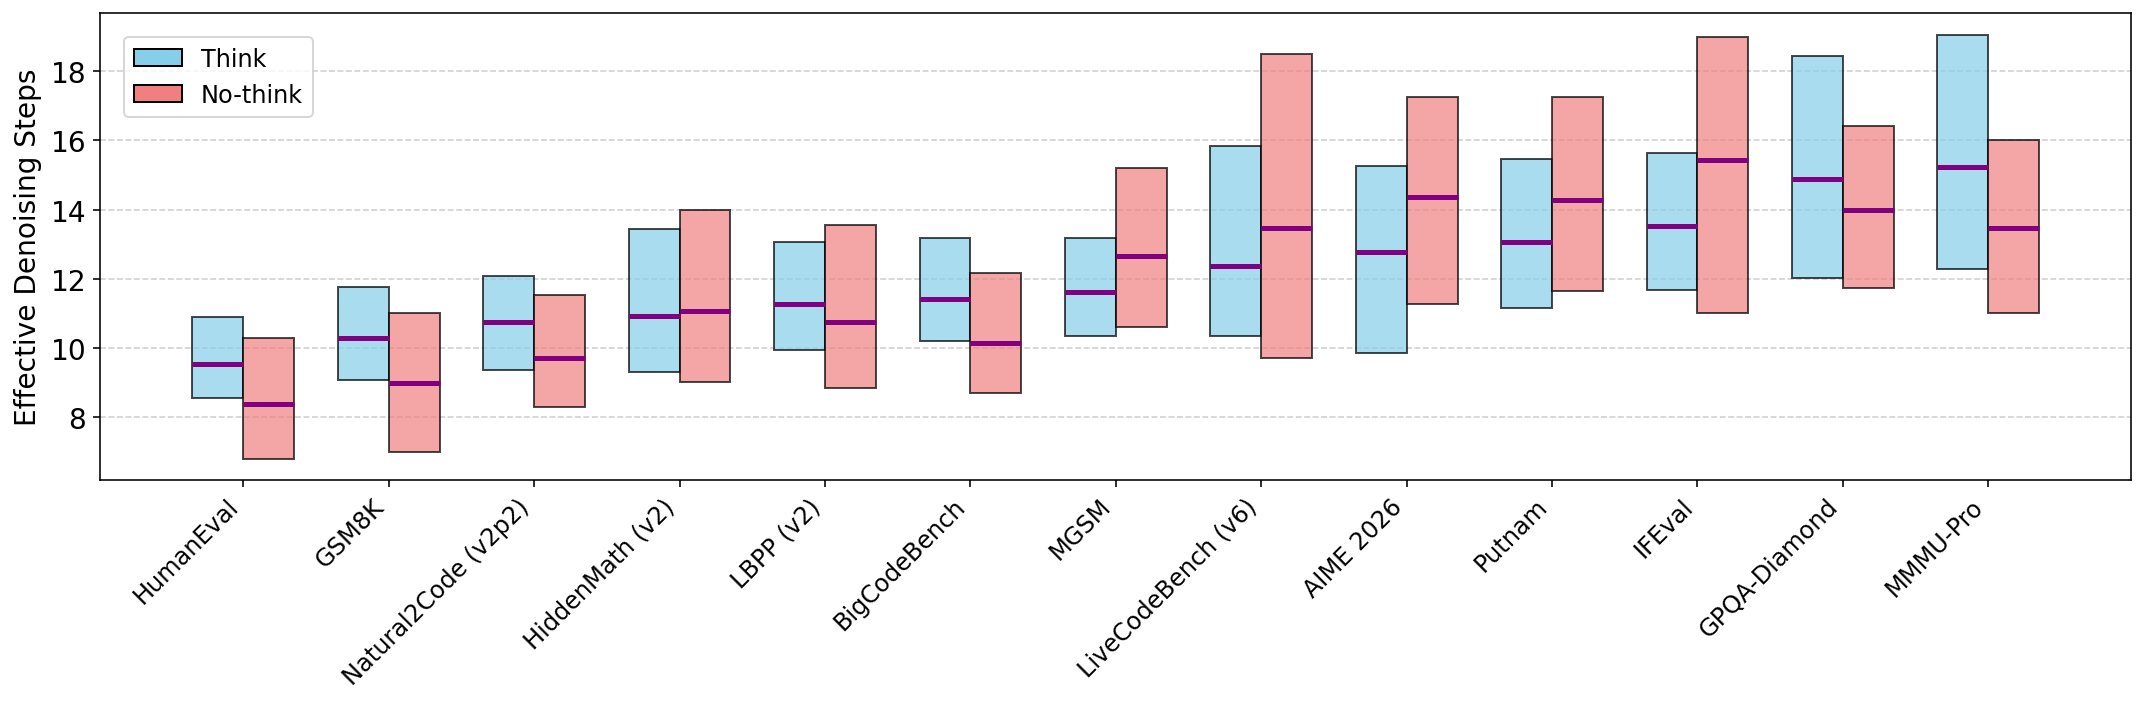
\includegraphics[width=1.0\linewidth]{assets/evals/boxplot_evals_dns.png}
    \caption{\textbf{Adaptive stopping은 DiffusionGemma가 작업 복잡도와 domain에 맞춰 denoising step 수를 동적으로 조절하게 한다.} effective denoising step(Equation~\ref{eq:effective_denoising_steps})의 중앙값과 1, 3사분위를 보고한다. 전체 benchmark와 latency 지표는 Table~\ref{tab:dg_td_latency}를 참조하라.}
    \label{fig:boxplot_evals_effective_denoising_steps}
\end{figure*}




\subsection{Inference 효율 지표} \label{sec:metrics}

adaptive stopping은 denoising step 수를 확률변수로 만들기 때문에, 우리는 denoising inference 효율을 정량화하기 위한 일련의 지표를 도입한다. 생성된 canvas 총수를 $K$, $k$번째 canvas에 실제로 수행된 denoising step 수를 $N_k \leq N$, 그 canvas에서 생성된 유효 token 수를 $C_k \leq C$라고 하자(즉 모든 $C$ token이거나, end-of-sequence token이 생성되면 그 첫 token까지). 먼저 Total Tokens를 전체 시퀀스에서 생성된 모든 유효 token의 합으로 정의한다:
\begin{equation}\label{eq:total_tokens}
\text{Total Tokens} \triangleq \sum_{k=1}^K C_k.
\end{equation}
\textbf{Total Denoising Steps}는 전체 생성 동안 수행된 denoising step의 절대 개수로 정의한다:
\begin{equation}\label{eq:total_denoising_steps}
   \text{Total Denoising Steps} \triangleq \sum_{k=1}^{K} N_k.
\end{equation}
각 denoising step은 고정된 계산 비용을 수반하므로, Total Denoising Steps는 end-to-end 생성 latency를 결정하는 주된 요인이다. 그러나 이 절대 지표는 전체 시퀀스 길이에 따라 본질적으로 함께 커지므로, 우리는 정규화된 모델 효율 지표도 평가한다. \textbf{Effective Denoising Steps}는 모든 canvas에 걸친 step 수의 token 가중 평균으로 정의한다:
\begin{equation}\label{eq:effective_denoising_steps}
   \text{Effective Denoising Steps} \triangleq \frac{1}{\text{Total Tokens}} \sum_{k=1}^K N_k C_k.
\end{equation}
우리는 유효 token 수로 가중치를 주는데, 이는 마지막 canvas가 부분적으로만 채워졌을 때 더 적은 denoising step을 필요로 하는 경향이 있어 지표가 아래로 치우치는 것을 막기 위해서다. adaptive stopping이 없다면 Effective Denoising Steps 지표는 항상 denoising budget $N$으로 환원된다는 점에 유의하라. 마지막으로 \textbf{Tokens Per Forward (TPF)}를 계산한다:
\begin{equation}\label{eq:tpf}
   \text{TPF} \triangleq \frac{\text{Total Tokens}}{\text{Total Denoising Steps} + K - 1},
\end{equation}
여기서 $K-1$ 항은 canvas 사이에서 새로 생성된 clean token을 인코딩하고 그 key-value 쌍을 KV cache에 추가하는 데 필요한 추가 forward pass 1회를 반영한다.

\subsection{유지된 Autoregressive 능력} \label{sec:retained_ar_capability}

DiffusionGemma는 Gemma 4와 정확히 같은 transformer 아키텍처를 공유하므로, 최종 DiffusionGemma 가중치는 원래 아키텍처에 그대로 다시 불러와 기반 모델과 동일하게 causal attention을 사용하는 표준 AR 생성을 수행할 수 있다. Section~\ref{sec:experiments}, Table~\ref{tab:model_comparison}에서 보이듯, 이 설정에서도 모델은 견고한 성능을 유지한다. AR mode의 성능 점수는 DiffusionGemma의 주된 text diffusion mode와, DiffusionGemma를 초기화한 기준 Gemma 4 checkpoint 성능 사이에 위치한다.



\section{Supervised Finetuning} \label{sec:sft}

\begin{figure}[!t]
    \centering
    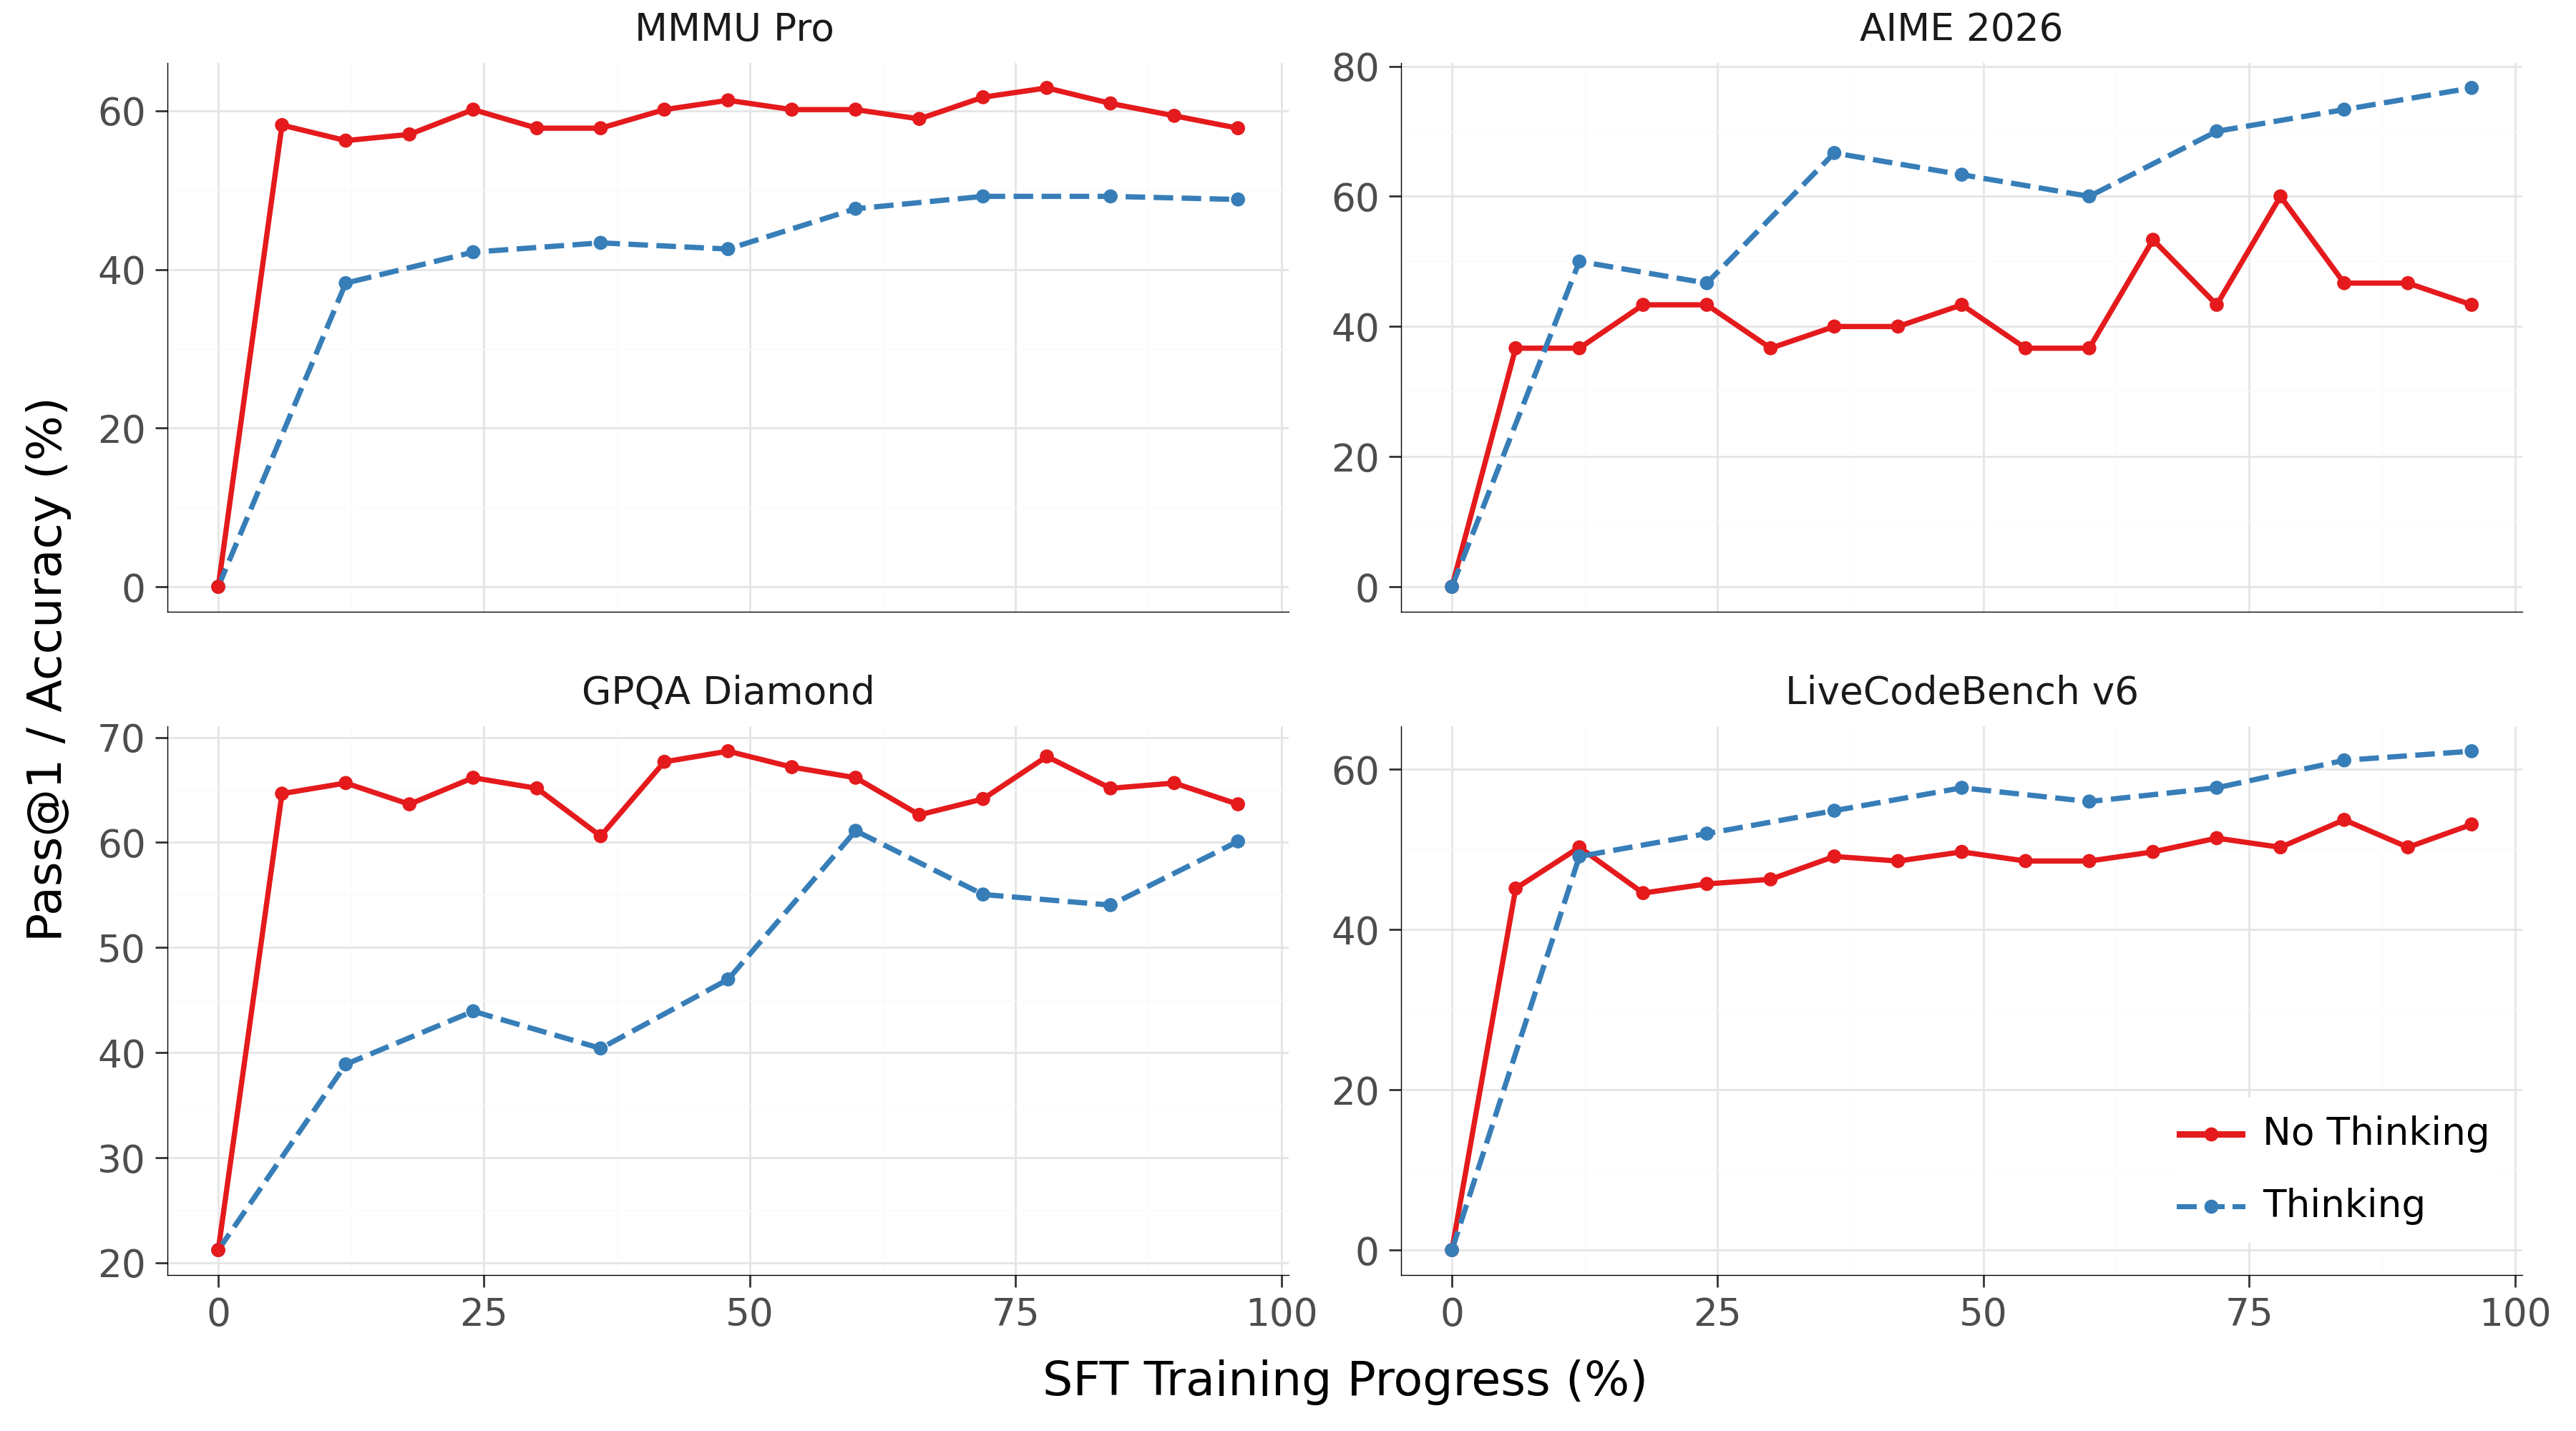
\includegraphics[width=0.9\linewidth]{assets/sft/sft_downstreams.png}
    \caption{\textbf{SFT 동안의 downstream 성능 변화.} SFT 이전에는 모델이 텍스트를 denoise하지 못한다. non-thinking mode에서 좋은 성능을 얻는 데에는 적당한 양의 SFT만으로도 충분하지만, thinking 행동을 학습하려면 더 긴 SFT가 중요하다. 결과는 adaptive stopping과 최대 $N=192$ denoising step을 사용하는 entropy-bounded sampling으로 얻었다.}
    \label{fig:sft}
\end{figure}

우리는 공개된 Gemma 4 26B A4B~\citep{gemmateam2026gemma4technicalreport} checkpoint에서 시작해, 모델이 noisy input으로부터 256 token 블록을 예측하도록 적응하는 확장된 finetuning 단계를 수행한다. 우리는 block-diagonal attention mask를 사용하여 각 블록 내부에서는 bidirectional attention을 허용하되, 모델이 다른 denoising 블록에 조건화되지 않도록 한다. 주어진 canvas에 대해 모델은 encoder KV cache를 통해 prompt와 이전(오염되지 않은) token에 조건화된다. corruption 과정으로는 discrete \emph{multinomial diffusion}을 사용하고, noisy token은 vocabulary에서 균등하게 sampling한다~\citep{hoogeboom2021argmax, austin2021structured}. 주어진 canvas에 대해 noise level $t \sim \unif[0, 1]$를 sampling하고, canvas의 각 token에 확률 $t$로 noise를 준다. prompt와 이전 canvas의 clean context $H$(KV cache를 통해 인코딩됨), self-conditioning 신호 $z_t$, noisy canvas $x_t$가 주어졌을 때, 모델은 자신의 예측과 학습 데이터에서 추출한 ground-truth canvas 사이의 cross-entropy loss를 최소화하도록 학습된다~\citep{gat2024discrete}:
\begin{equation}
    L(\theta) = - \sum_{i=1}^C \log p_{\theta}(x_0^i \mid x_t, z_t, H),
\end{equation}
여기서 위첨자 $i$는 canvas 차원의 인덱스를 뜻하며, $p_\theta$는 신경망 출력 logits에 대한 softmax 변환으로 매개변수화된다. Figures~\ref{fig:sft}와~\ref{fig:average_sft}에서 보듯, denoising 성능은 학습 초기에 빠르게 향상된 뒤 log-linear한 성능 향상 추세로 들어간다. thinking 성능은 확장된 SFT의 이점을 받는데, 이는 모델이 처음에는 일관된 reasoning trace를 유지하는 데 어려움을 겪고 종종 stuttering이나 cycle로 붕괴하기 때문이다. 이는 언어 모델이 reasoning을 내재화할 때 흔히 마주치는 과제다~\citep{zelikman2024quiet}.

\begin{figure}[!t]
    \centering
    \begin{minipage}[c]{0.6\linewidth}
        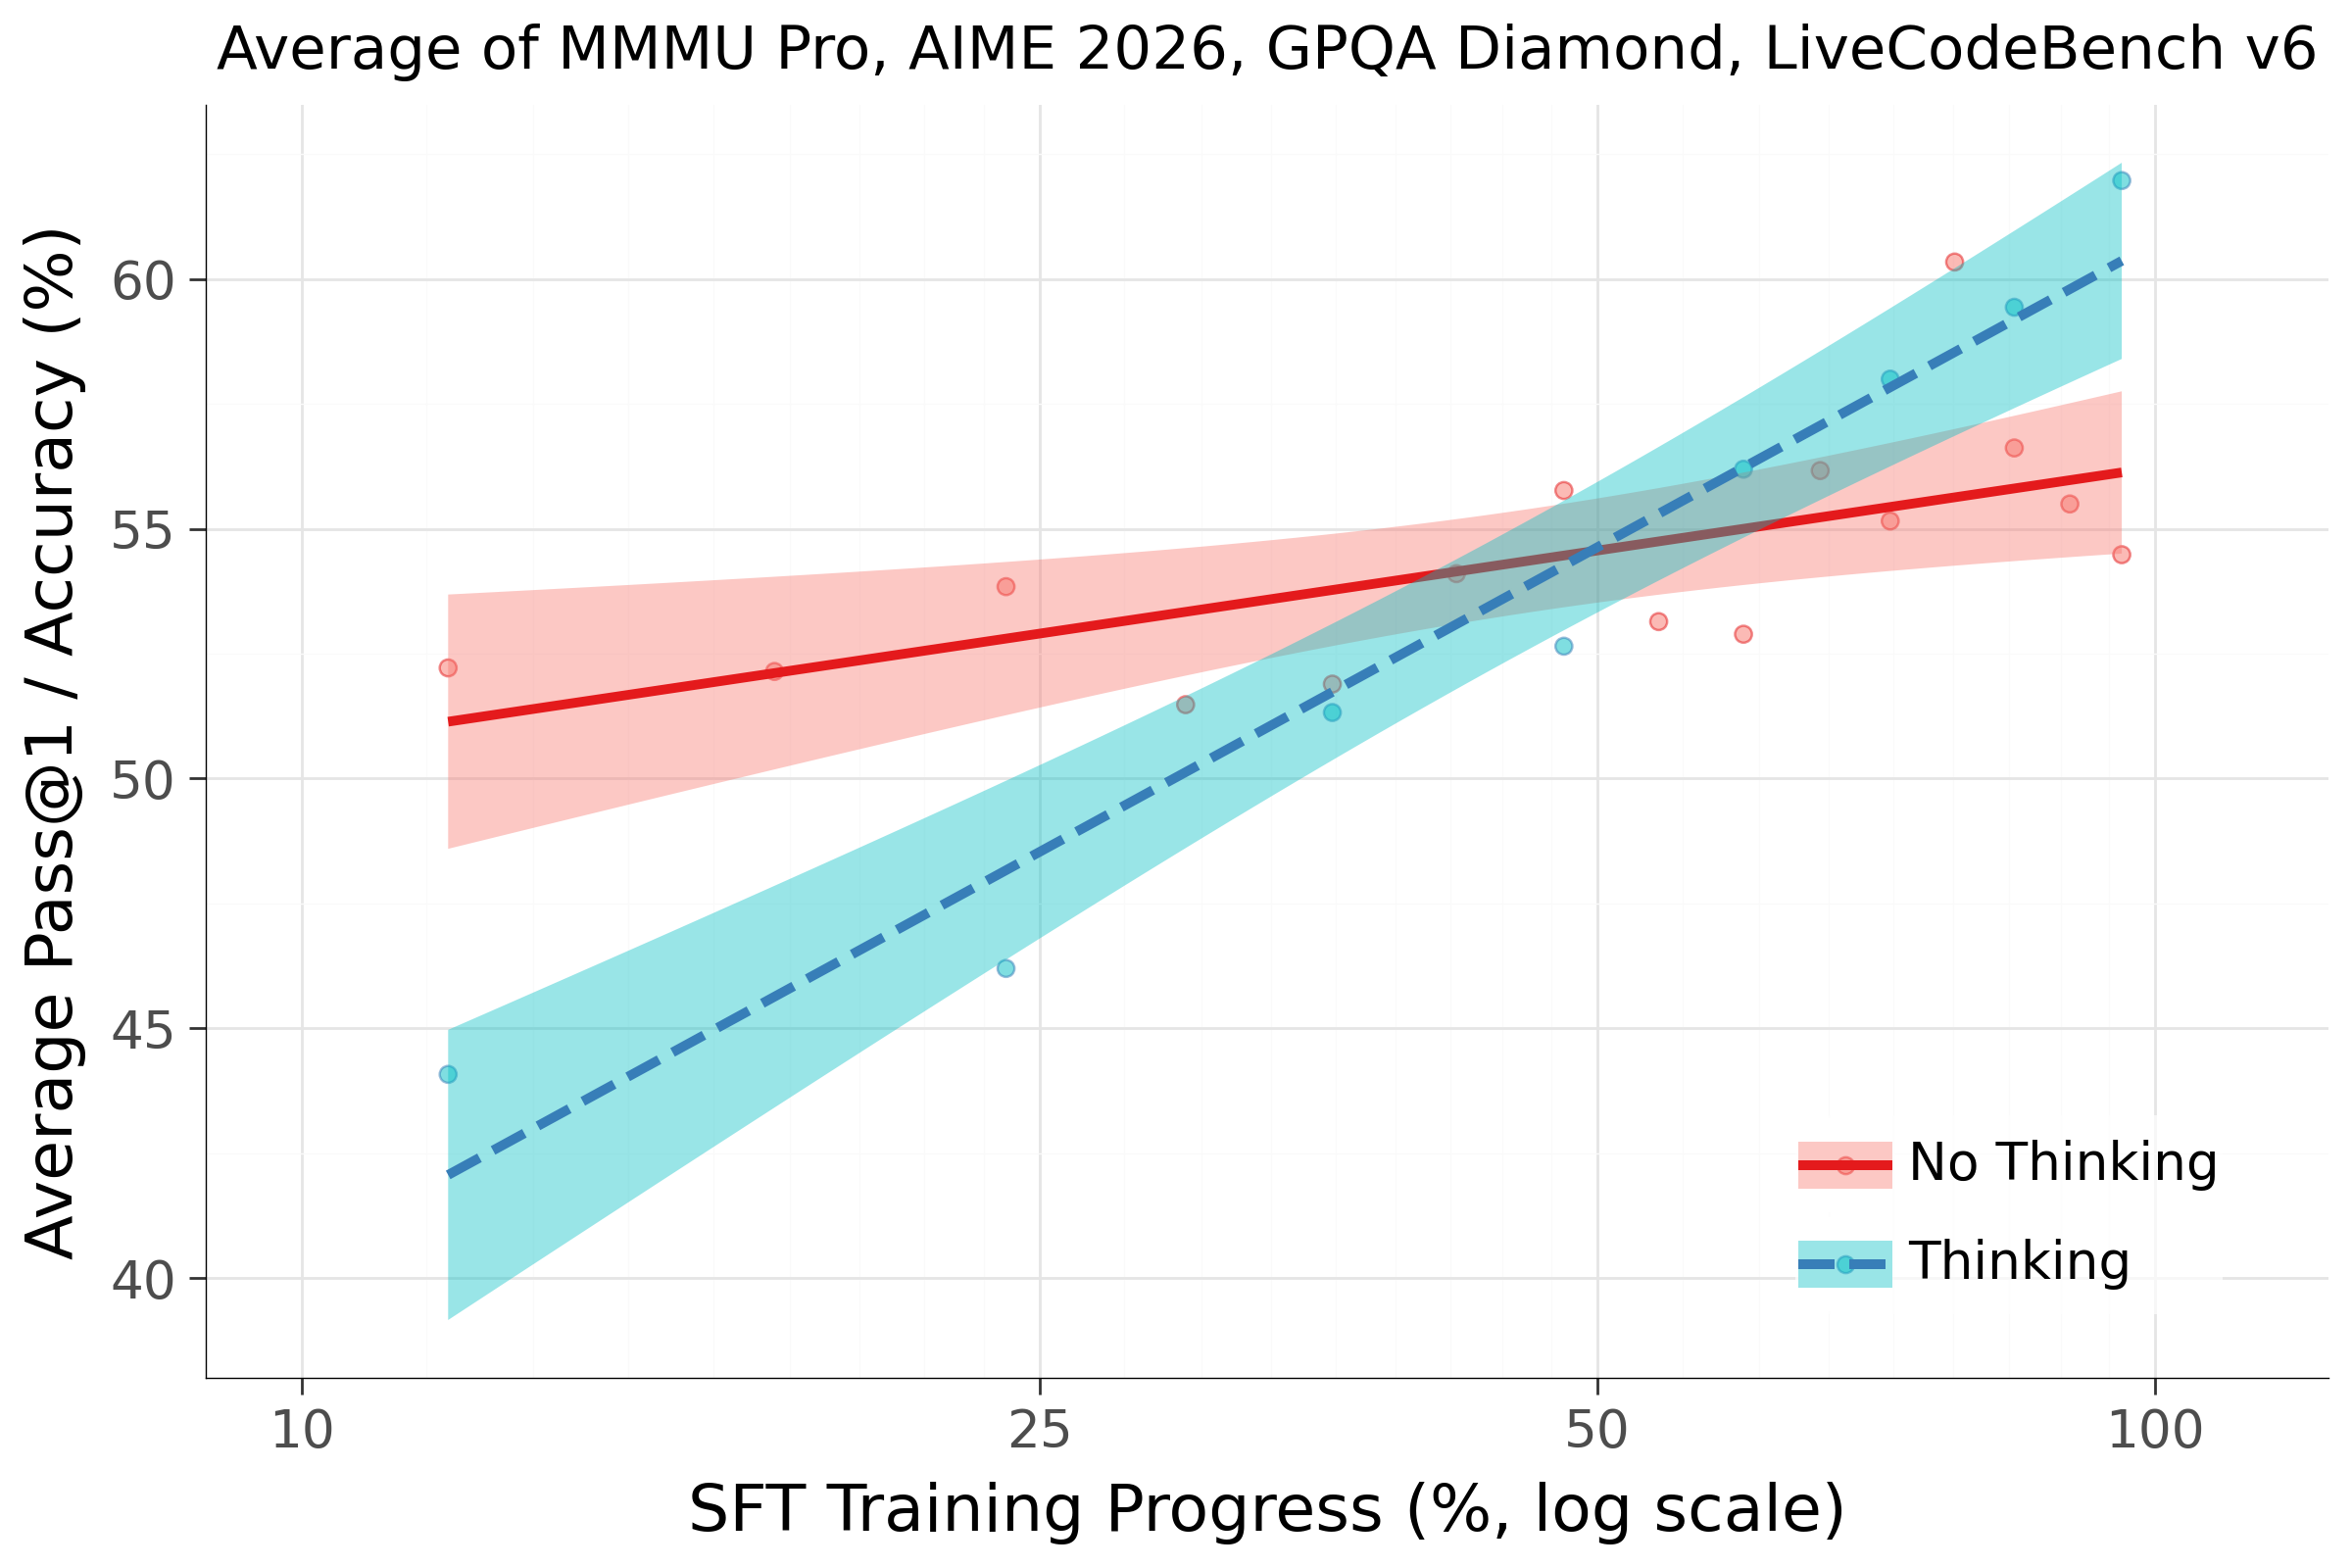
\includegraphics[width=0.95\linewidth]{assets/sft/sft_average_downstreams.png}
    \end{minipage}\hfill
    \begin{minipage}[c]{0.35\linewidth}
        \caption{\textbf{SFT 동안의 downstream 성능은 학습 진행에 따라 log-linear하게 향상된다.} thinking 성능의 log-linear 추세는 더 낮은 지점에서 시작하지만 non-thinking mode보다 더 가파른 기울기를 보인다. 결과는 adaptive stopping과 최대 $N=192$ denoising step을 사용하는 EntropyBounded sampler로 얻었다.}
        \label{fig:average_sft}
    \end{minipage}
\end{figure}


\section{Sampler Distillation \& Reinforcement Learning} \label{sec:sdrl}


SFT 단계 이후, 모델은 많은 denoising step을 사용할 때 강한 생성 품질을 달성한다. 그러나 고급 reasoning 및 coding 작업에서는 기준 AR 모델보다 성능이 다소 낮다. 더 치명적인 문제는 초저지연 inference에 필요한 few-step regime로 들어가면 생성 품질이 무너진다는 점이다. 이를 해결하기 위해 우리는 두 가지 개선을 동시에 노린다. 모델의 지능을 끌어올리면서, 동시에 denoising trajectory를 압축하는 것이다.

전통적으로 이 두 목표를 달성하려면 reward-driven alignment와 sampler distillation을 별도 단계로 다루는 분리된 multi-stage 파이프라인이 필요하다. 우리는 이를 \textbf{sampler distillation \& reinforcement learning} (\sdrl)이라 부르는 통합 \textit{online learning} 단계로 우회하며, 이 단계는 두 축을 동시에 최적화한다. 결합 목적함수에 기반하여, 단일 gradient update가 다음을 함께 밀어 올린다:

\begin{enumerate}[topsep=0pt]
    \item \textbf{Reward maximization}: AR 및 diffusion 모델을 위한 표준 RL과 유사하게 절대적인 생성 품질과 alignment를 높인다 \citep{black2024training, liu2025flow, zheng2025diffusionnft, zhao2025d1, ma2025reinforcement, wallace2023diffusion, fan2023dpok, clark2024directly, dong2023raft, lee2023aligning}.
    \item \textbf{Sampler distillation}: 이 고품질 생성을 few-step regime으로 사상하여, 반복형 diffusion 프레임워크에 고유한 압축 과제를 해결한다 \citep{salimans2022progressive, song2023consistency, deschenaux2025beyond, fu2025learnable, luo2023latent, sauer2024adversarial, liu2023instaflow, yin2024distribution, hoogeboom2026beyond}.
\end{enumerate}


\paragraph{Training setup.} 우리는 Gemma~4 RL recipe \citep{gemmateam2026gemma4technicalreport}에서 사용한 데이터 분포를 우리의 사용 사례에 맞게 조정한다. thinking과 non-thinking mode를 모두 포괄하는 이 설정은 helpfulness, 수학적 reasoning, coding, instruction-following 등 다양한 능력 전반의 개선을 목표로 한다. SFT 가중치에서 초기화된 모델은 온라인 teacher로 동작하며, 높은 최대 denoising step 수와 완만한 temperature annealing으로 설정된 sampler를 사용해 denoising trajectory를 생성하고 이를 고품질 기준으로 삼는다. \sdrl 결합 목적함수는 이 trajectory를 활용해 보상을 동시에 최대화하고 sampler distillation을 추진함으로써, 모델의 최고 품질 출력을 few-step regime으로 압축한다.


\begin{figure*}[!t]
    \centering
    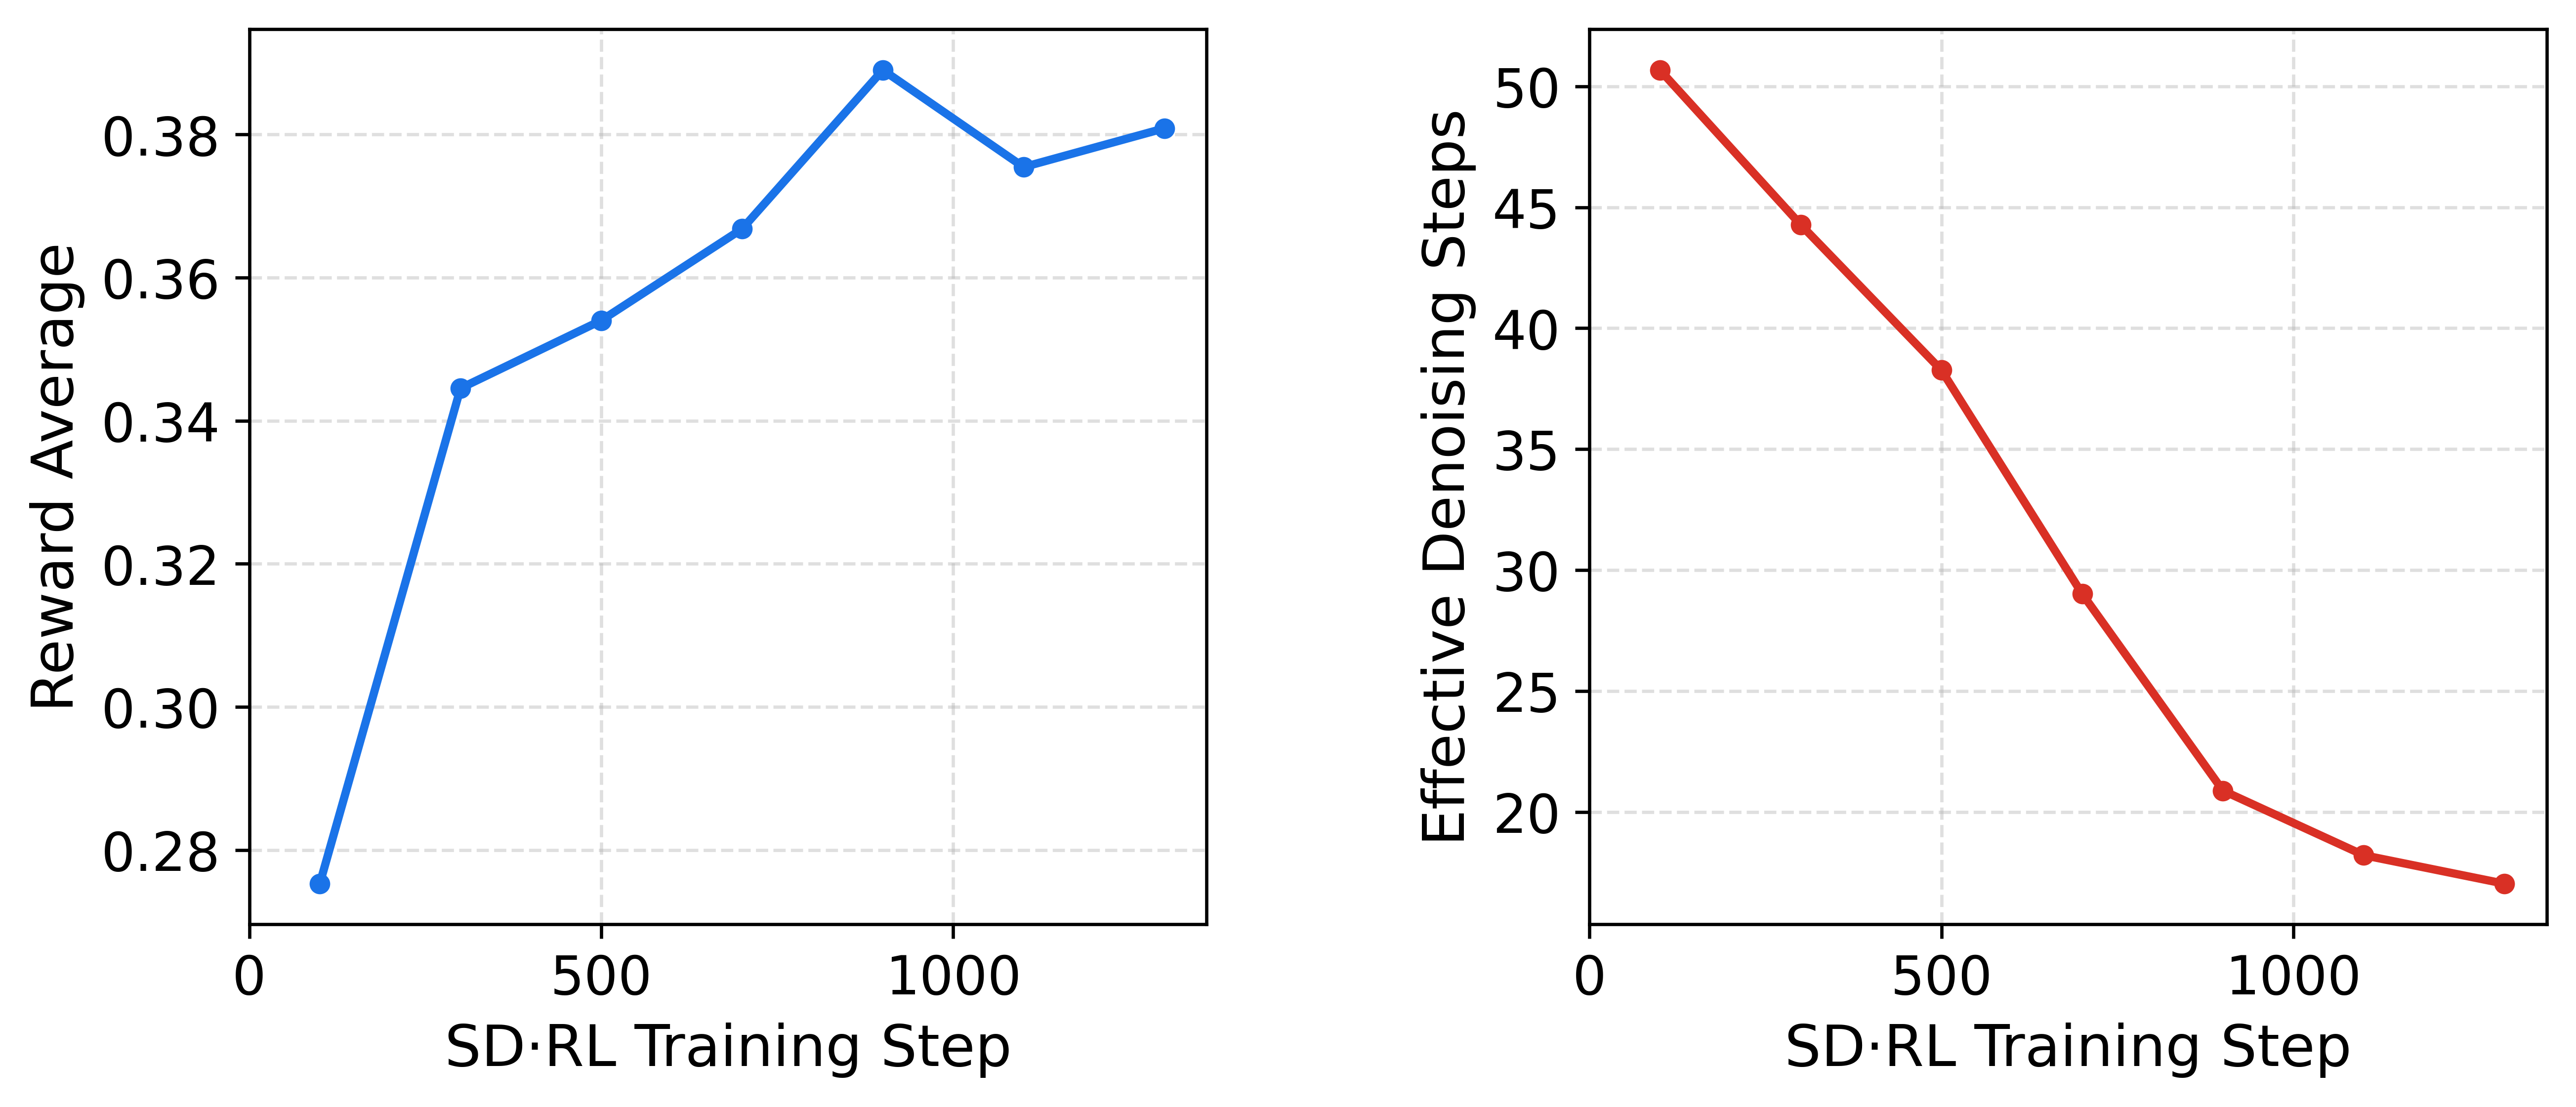
\includegraphics[width=0.8\linewidth]{assets/sdrl/sdrl_training.png}
    \caption{
        \textbf{\sdrl 학습은 온라인 teacher의 평균 보상을 높이는 동시에 effective denoising step 수를 줄인다} (학습 지표는 200 step 단위 bucket으로 표시). 이 두 효과가 함께 모델의 품질-속도 Pareto frontier를 밀어 올린다.
    }
    \label{fig:rl-training-metrics}
\end{figure*}



\paragraph{Training dynamics \& implicit curriculum effect.} Figure~\ref{fig:rl-training-metrics}에서 보이듯, \sdrl 학습이 진행되면서 두 가지 상호보완적 동학이 나타난다. 첫째, 온라인 teacher의 평균 보상이 꾸준히 증가하여 기본 능력이 향상됨을 보여 준다. 둘째, adaptive stopping 메커니즘의 도움으로 온라인 teacher는 이러한 높은 보상을 달성하는 데 점점 더 적은 effective denoising step만 필요로 하게 된다. 이러한 가속은 \sdrl 목적함수가 모델의 predictive entropy를 체계적으로 낮추기 때문에 일어난다. 중요한 점은 reward objective와 adaptive stopping의 상호작용이 curriculum learning 효과를 유도한다는 것이다. 학습 초반에는 높은 predictive entropy가 adaptive stopping 발동을 지연시킨다. 모델의 확신이 올라가고 entropy가 내려가면 adaptive stopping이 더 이르게 발동한다. 이는 학습 분포를 점점 더 짧은 denoising trajectory 쪽으로 자연스럽게 이동시키며, 알고리즘이 자신의 sampler distillation 속도를 동적으로 조절하게 한다. 따라서 AR 모델용 RL과 달리, \sdrl 단계는 reward 지표가 plateau에 도달한 뒤에도 오래 지속할수록 큰 이득이 있다. entropy가 계속 감소하면 그것이 곧바로 추가적인 inference 속도 향상으로 이어지기 때문이다.


\begin{figure*}[!t]
    \centering
    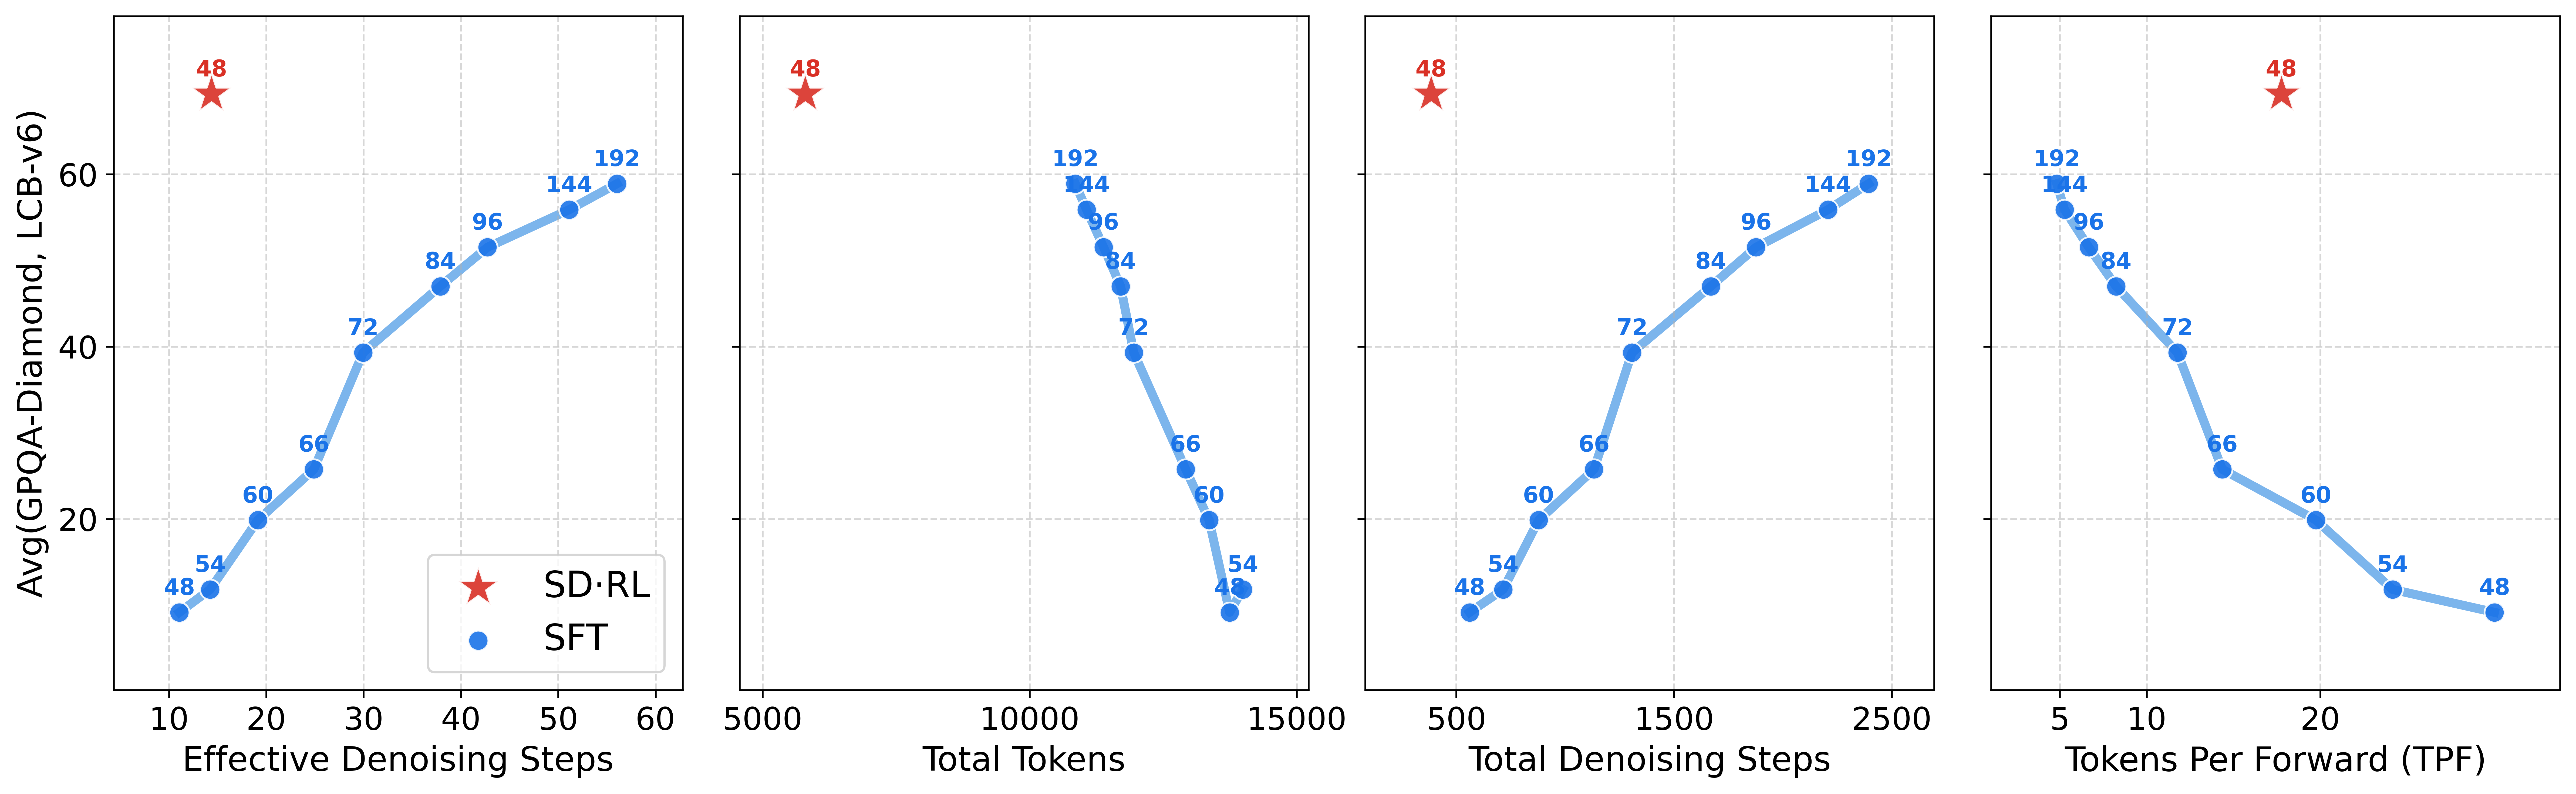
\includegraphics[width=1.0\linewidth]{assets/sdrl/pareto_sdrl_vs_sft.png}
    \caption{\textbf{\sdrl은 품질-속도 Pareto frontier를 크게 전진시킨다.} \sdrl 설정은 최대 $N=48$ denoising step을 사용하는 DiffusionGemma sampler를 사용한다. SFT frontier는 $N$을 48에서 192까지 sweep하여 얻었다(더 높은 $N$은 더 완만한 temperature annealing을 뜻한다). 품질(y축)과 inference 효율(x축, Section~\ref{sec:metrics} 참조)은 모두 thinking mode에서 GPQA-Diamond와 LiveCodeBench-v6 평균을 3개 seed에 걸쳐 다시 평균하여 계산했다.}
    \label{fig:pareto-rl-vs-sft}
\end{figure*}


\paragraph{Improved speed-to-intelligence Pareto frontier.} Figure~\ref{fig:pareto-rl-vs-sft}에서 보듯, \sdrl 학습은 SFT checkpoint가 세운 Pareto frontier를 크게 확장한다. 품질 축에서는 GPQA-Diamond와 LiveCodeBench-v6 결합 점수를 10점 개선하고, 효율 축에서는 TPF를 5에서 거의 20으로 네 배 늘려 초저지연 inference를 가능하게 한다.

Figure~\ref{fig:pareto-rl-vs-sft}에서 보듯, 기본 DiffusionGemma sampler(최대 $N=48$ denoising step)로 SFT checkpoint를 평가하면 downstream 정확도는 낮고 effective denoising step도 인위적으로 낮게 나온다. 이 반직관적 현상은 SFT 모델이 이 제한된 step regime에서 반복적 token loop로 자주 붕괴하기 때문이다. 일단 loop에 빠지면 predictive entropy가 붕괴하고, 그 결과 adaptive stopping 메커니즘이 너무 이르게 발동한다. Figures~\ref{fig:gpqa-rl-example-biology}와 \ref{fig:gpqa-rl-example-quantum}(Appendix~\ref{sec:samples_before_after_sdrl})는 GPQA-Diamond benchmark의 생성 샘플을 통해 이런 붕괴가 어떻게 나타나는지 보여 준다. SFT 모델은 유효하고 논리적인 reasoning trace로 시작하지만 갑자기 token 반복 loop로 무너진다. 반대로 \sdrl 이후 샘플은 이런 퇴행적 함정을 피해, 최소 latency에서도 일관된 reasoning을 유지한다.


\paragraph{\sdrl specialization in the few-step regime.} SFT checkpoint에서는 downstream 성능이 denoising의 최대 step 수 $N$에 따라 192까지 일관되게 증가하며, 이 지점에서 denoising은 대략 any-order autoregressive에 가까워진다. \sdrl 이후에는 $N$에 따른 scaling 거동이 더 빠르게 좋아지고 더 일찍 plateau에 도달한다. 성능은 $N=48$까지 꾸준히 개선되지만, 그 이후로는 수익 체감이 나타난다(Figure~\ref{fig:score_vs_dns}). 이런 이른 포화는 \sdrl 목적함수가 predictive entropy를 공격적으로 최소화해 모델을 few-step regime에 명시적으로 특화시키기 때문에 나타난다.



\paragraph{Emergent conciseness.}
우리의 \sdrl 최적화에서 나타나는 emergent property 중 하나는, 모델이 간결하고 token-efficient한 출력을 내도록 장려된다는 점이다. 이는 더 긴 reasoning trace를 유도함으로써 보상을 극대화하는 경우가 잦은 AR 모델용 RL과 대조적이다. 최종 checkpoint는 SFT checkpoint보다 거의 $2\times$ 짧은 출력을 만든다(Figure~\ref{fig:pareto-rl-vs-sft}). 이는 모델이 확장된 reasoning과 함께 오는 일부 능력 향상을 포기한다는 뜻이지만, inference 속도 향상에는 배수 효과로 작용한다. 전체 token 수가 적고 canvas당 effective denoising step도 적다는 점이 결합되어 매우 낮은 end-to-end latency를 직접 만들어 낸다. DiffusionGemma는 우리의 eval suite 전반에서 Gemma 4 AR baseline이 사용하는 전체 forward pass의 $5\%$ 미만만 필요로 한다.

\begin{figure*}[t]
    \centering
    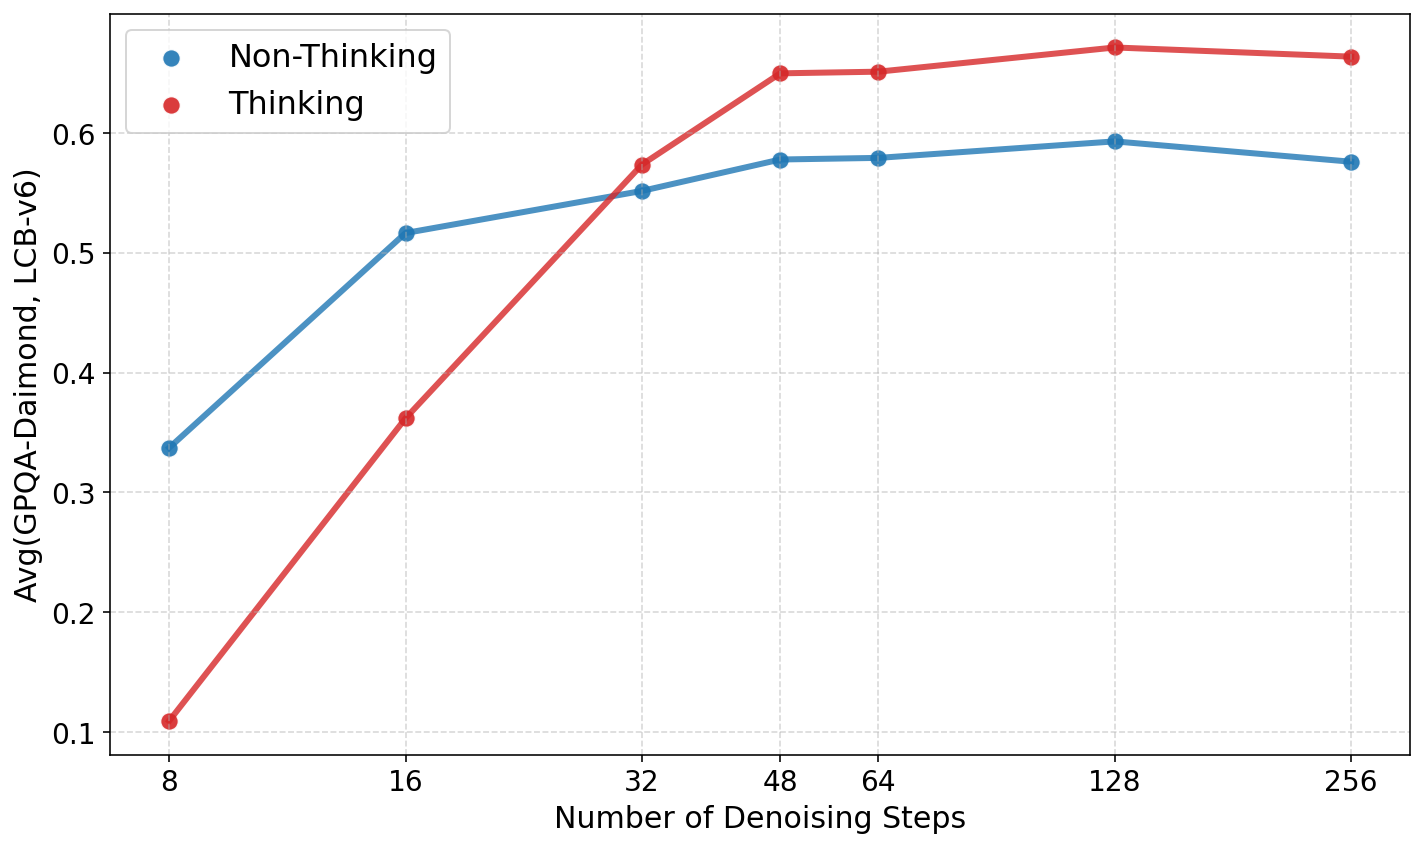
\includegraphics[width=0.6\linewidth]{assets/sdrl/performance_vs_denoising_steps.png}
    \caption{\textbf{Adaptive stopping과 temperature annealing 없이 본 denoising step 수 $N$ 대비 성능.} 성능은 GPQA-Diamond와 LiveCodeBench-v6 점수 평균(3 seeds)으로 측정한다. 조기 중단과 temperature annealing의 교란 효과를 제거하기 위해 adaptive stopping을 비활성화하고 temperature $\tau_t = 1$을 사용했다.}
    \label{fig:score_vs_dns}
\end{figure*}


\section{Inference 최적화} \label{sec:inference_optimizations}

앞선 절들은 SFT와 \sdrl 파이프라인을 통해 forward pass당 생성 token 수를 최대화하는 데 초점을 맞췄다. 이제 우리는 보완적인 축으로 이동한다. 즉, GPU 수준의 표적 최적화를 통해 각 forward pass의 wall-clock 비용을 최소화하는 것이다. 근본적으로 text diffusion이 AR decoding보다 가지는 처리량 이점은 경쟁하는 두 양에 의해 결정된다. 한편으로 각 denoising step은 $\mathrm{TPF}$개의 token을 디코딩하므로, AR baseline보다 $\mathrm{TPF}$배 적은 forward pass만 필요하다. 다른 한편으로 각 forward pass는 256 token canvas를 처리하기 때문에, 각 step은 $r$배 느려지고, 따라서 AR baseline 대비 전체 처리량은 $\mathrm{TPF}/r$가 된다. hardware 최적화는 이 forward pass 오버헤드를 크게 줄일 수 있다.

\paragraph{Low batch size serving.} text diffusion inference는 생성 token당 AR 모델보다 더 많은 floating-point operation(FLOP)을 요구하지만, forward pass 수는 훨씬 적다. 현대 하드웨어 가속기에서의 LLM serving은 보통 KV cache 용량과 memory bandwidth에 크게 좌우되는 memory-bound 문제이기 때문에~\citep{kwon2023efficient, pope2023efficiently}, 메모리 전송 감소가 더 높은 계산 비용을 상쇄하는 latency 이점을 만든다. 그 결과 text diffusion은 low-batch-size 시나리오에서 매우 효과적이며, 사용 가능한 compute capacity를 활용해 요청당 latency를 최소화한다. 단순화를 위해 우리의 분석은 DiffusionGemma의 단일 요청 inference 처리량(batch size 1)에 초점을 맞추고, 이를 AR 대응 모델인 Gemma 4 26B A4B와 직접 비교한다. 참조 inference 구현은 HuggingFace Transformers~\citep{diffusiongemma2026hf}와 vLLM~\citep{vllm2026diffusiongemma}에서 제공된다.

\begin{figure}[htbp]
    \centering
    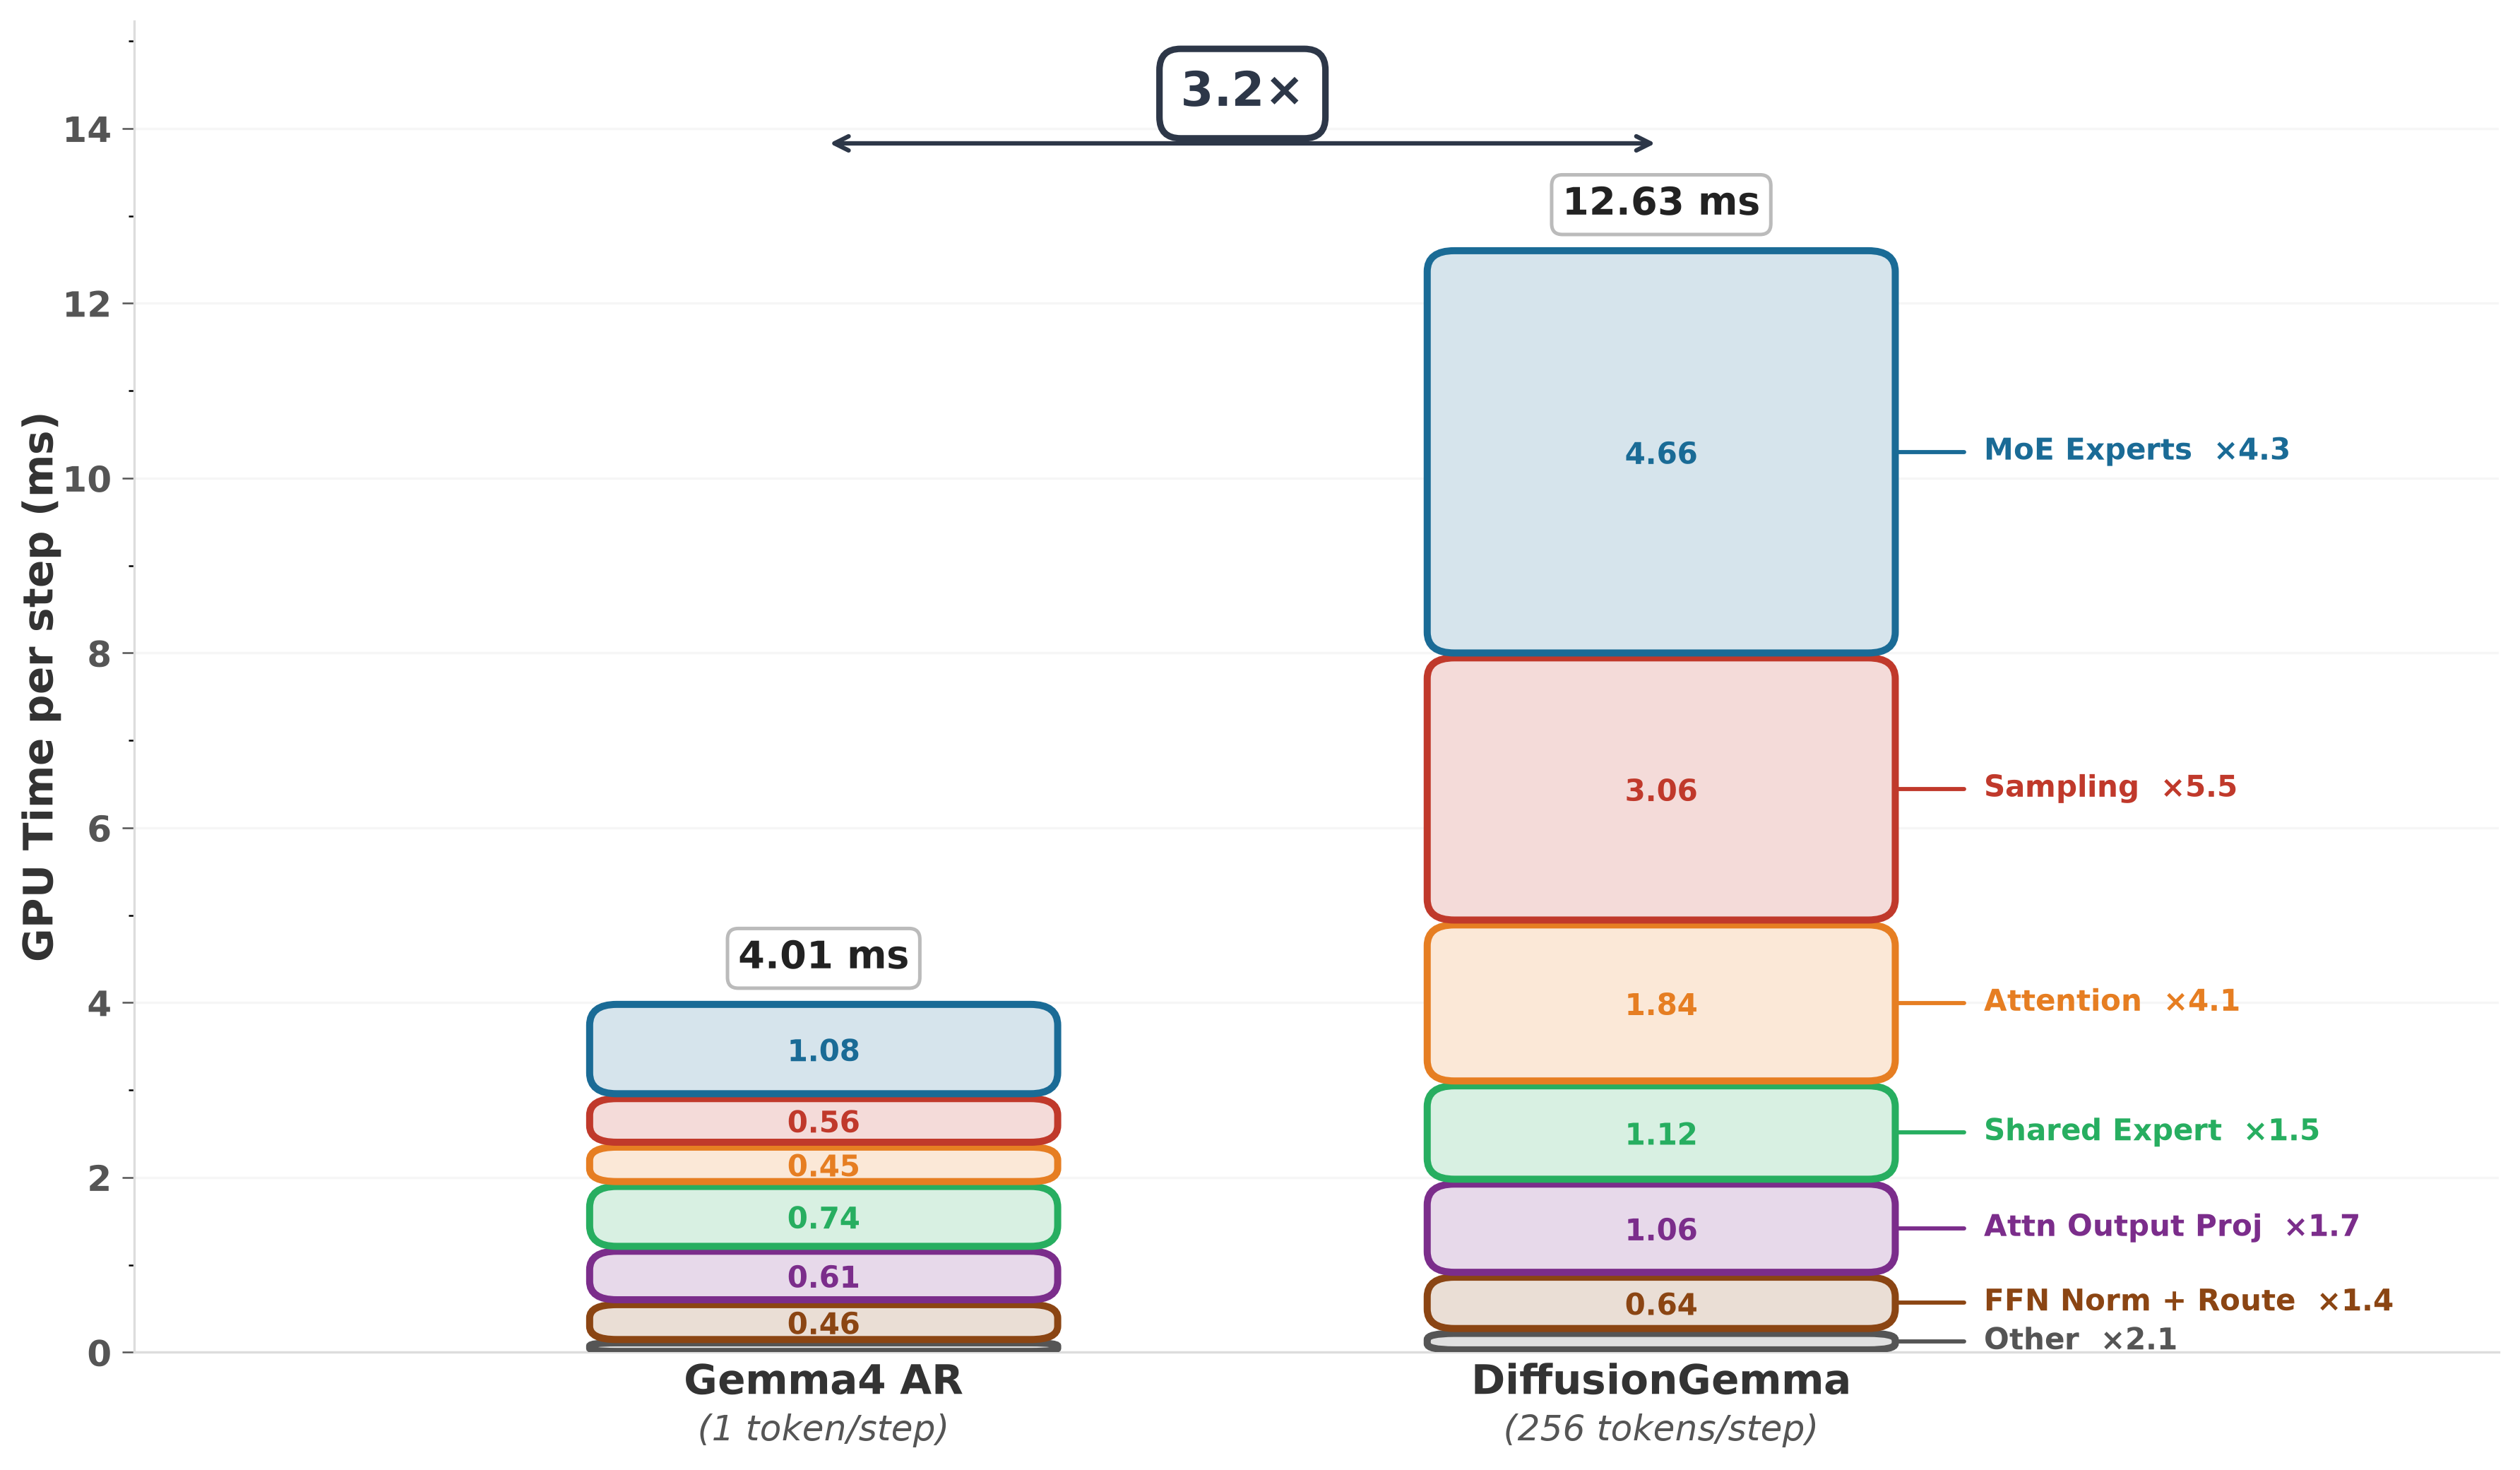
\includegraphics[width=1\linewidth]{assets/inference_figures/op_breakdown_plot8.png}
    \caption{
        \textbf{Step당 GPU 시간 분해: DiffusionGemma는 단일-token AR 생성 대비 step당 latency가 3.2$\times$ 증가하는 데 그치면서 step마다 256 token을 처리한다.} H100, FP8 정밀도, 입력 4096 token과 출력 1024 token 조건에서 단일 요청(batch size 1)을 서빙한 결과다.
    }
    \label{fig:inference-comparison}  
\end{figure}

\paragraph{GPU time breakdown.} Figure~\ref{fig:inference-comparison}은 두 모델의 step당 GPU kernel 시간 분해를 보여 준다. 우리는 모델 고유의 병목을 분리하기 위해 end-to-end latency보다 GPU kernel 시간에 초점을 맞춘다. 각 모델에서 end-to-end latency는 detokenization과 기타 CPU 측 serving overhead 때문에 GPU kernel 시간보다 약 1\,ms 정도 더 크며, 이 격차는 Gemma 4 AR과 DiffusionGemma 모두에서 비슷하다. DiffusionGemma의 각 step은 $256\times$ 더 많은 token을 처리하지만, 단일-token AR step보다 겨우 $3.2\times$ 느릴 뿐이다. 이 시간 차이는 주로 세 연산, 즉 mixture-of-experts (MoE), sampling, attention에서 기인한다. 다른 연산(예: shared expert, attention output projection 등)은 최대 $2\times$ 정도만 느려진다.

\begin{itemize}[topsep=0pt]
    \item \textbf{MoE.} 단일 요청을 서빙할 때 MoE layer 계산은 memory-bound이며, 실행 시간은 sparse MoE 모델 서빙 시 잘 알려진 병목인 high-bandwidth memory로부터 expert 가중치를 옮기는 비용에 지배된다~\citep{rajbhandari2022deepspeedmoe, huang2024efficient}. Gemma 4 AR 모델에서는 token당 MoE layer마다 고유 expert 8개만 활성화된다. DiffusionGemma 모델에서는 PG-19 benchmark~\citep{rae2020compressive}에서 측정했을 때, 256 token canvas당 MoE layer마다 평균 약 84개의 고유 expert가 활성화된다.\footnote{데이터셋은 \url{https://github.com/google-deepmind/pg19}에서 제공된다.} forward pass당 더 많은 expert를 활성화하면 MoE kernel이 $4.3\times$ 느려진다. 이는 speculative decoding의 verification에서 발생하는 것과 같은 종류의 패널티지만, 더 큰 token 병렬성으로 확대된 형태다. dense architecture라면 이 오버헤드는 사라지고, step당 feed-forward network 둔화는 $2\times$ 미만으로 줄어들 것이다.
    \item \textbf{Sampling.} AR의 단일-token softmax-and-sample을 넘어서, text diffusion sampling은 추가 연산을 요구한다. 대표적으로 self-conditioning embedding matmul과 256 token 전체 canvas에 대한 softmax가 있다(Algorithm~\ref{alg:sampling} 참조). 이 연산들은 vocabulary 차원 262k에 대해 full precision으로 수행된다. 그 결과 text diffusion sampling은 3.06ms가 걸리는 반면 AR sampling은 0.56ms에 불과하다. 우리는 커뮤니티가 더 쉽게 확장할 수 있도록, 손수 작성한 GPU kernel 대신 \texttt{torch.compile}로 최적화한 표준 PyTorch primitive를 사용해 sampling을 구현했다.
    \item \textbf{Attention.} AR와 달리 DiffusionGemma는 256 token canvas에 대해 bidirectional attention을 사용한다. 따라서 AR 모델이 사용할 수 있는 빠른 단일-token decoding attention은 활용할 수 없지만, 고도로 최적화된 FlashAttention-4 kernel \citep{dao2022flashattention, zadouri2026flashattention4}은 활용할 수 있다. 이러한 최적화 아래에서 attention 연산은 Gemma 4 AR 모델보다 DiffusionGemma 모델에서 $4\times$ 느리다.
\end{itemize}

\paragraph{Eliminating CPU-GPU synchronization.} DiffusionGemma를 서빙할 때는 추가적인 복잡성이 있다. denoising step은 adaptive stopping에 의존하고, 서로 다른 attention mask를 요구하는 두 종류의 forward pass(denoising step과 KV cache update)가 같은 batch 안에서 발생할 수 있기 때문이다. 요청 latency를 최소화하려면 이 복잡성을 추가적인 CPU-GPU synchronization을 유발하지 않고 오직 GPU 연산만으로 처리하는 것이 중요하다. 이는 비동기 스케줄링을 text diffusion 모델로 확장하고 sequence별 causal attention flag를 도입함으로써 달성된다(자세한 내용은 \citealp{vllm2026diffusiongemma} 참조).

\paragraph{Batch size 1 서빙에서의 처리량.} text diffusion 모델의 decoding 처리량은 다음 식으로 계산한다:
\begin{equation}\label{eq:tps}
\text{TPS} \triangleq \dfrac{\text{TPF}}{t_{\text{fwd}}},
\end{equation}
여기서 TPS는 Tokens Per Second, TPF는 Tokens Per Forward(Equation~\ref{eq:tpf} 참조), $t_{\text{fwd}}$는 단일 denoising step에 필요한 시간으로, context 길이에 따라 달라진다(attention 때문). H100 GPU(FP8 정밀도)에서, 입력 4096 token과 출력 1024 token을 갖는 단일 요청을 서빙할 때 DiffusionGemma의 단일 denoising step은 평균 $t_{\text{fwd}}=13.56\text{ms}$가 걸린다(end-to-end 기준이며, step당 GPU 시간은 12.63ms, Figure~\ref{fig:inference-comparison} 참조). TPF는 작업에 따라 달라진다. Table~\ref{tab:model_comparison}에 보고된 7개 benchmark 전반의 평균 TPF인 19.74를 가정하면, 모델의 평균 decoding 처리량은 1456 TPS다. 이는 같은 장치 설정에서 Gemma 4 AR 모델(204 TPS)보다 $7.1\times$, MTP가 있는 AR 모델(303 TPS)보다 $4.8\times$ 빠르다.

\begin{figure}[!t]
    \centering
    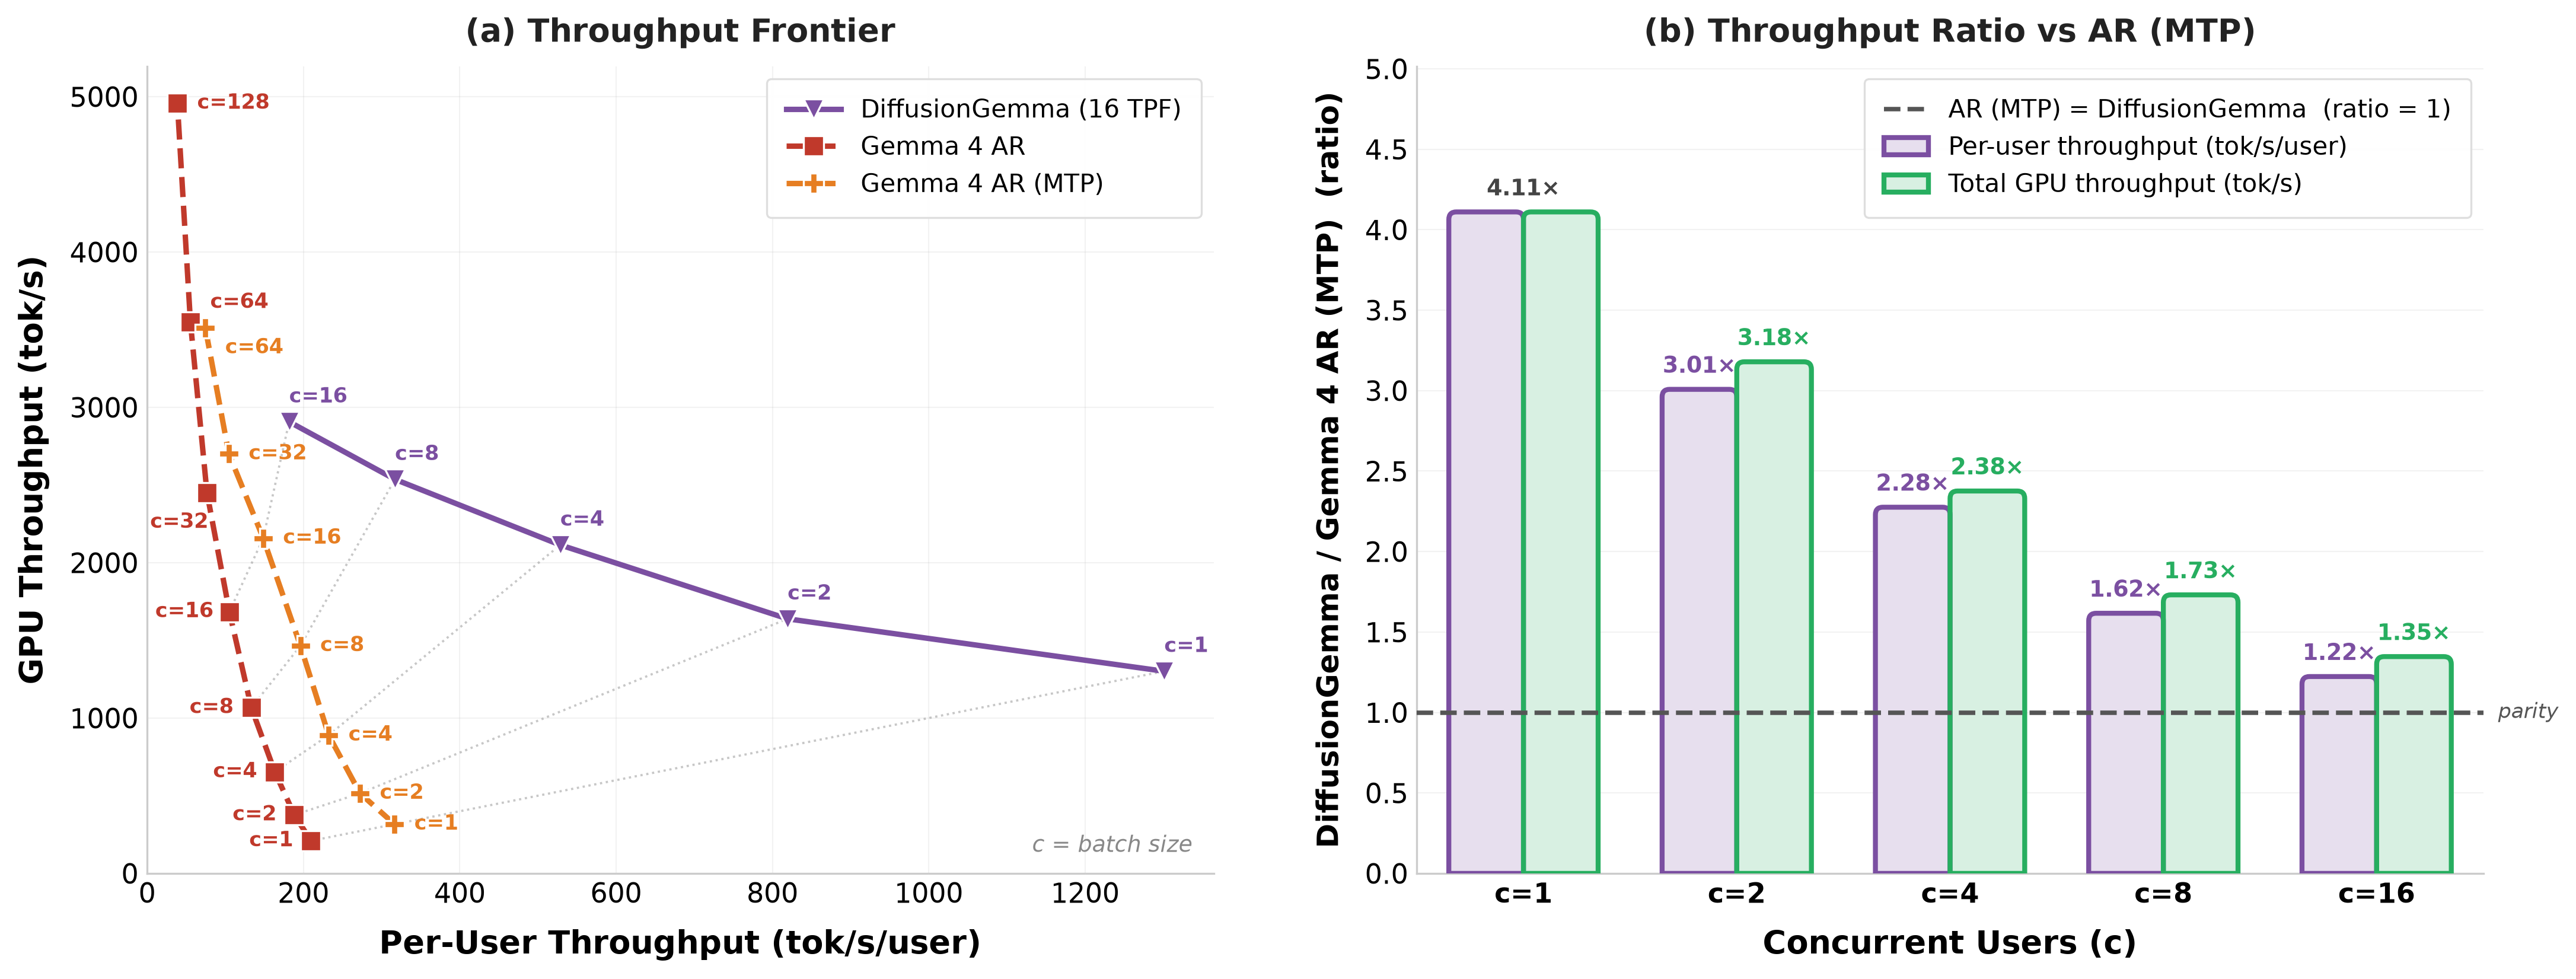
\includegraphics[width=1\linewidth]{assets/inference_figures/throughput_plot_merged11.png}
    \caption{
        \textbf{Gemma 4 AR 모델(MTP 유무)과 DiffusionGemma의 총 처리량 및 사용자당 처리량 절충 관계.} batch size가 작은 구간에서 DiffusionGemma는 사용자당 TPS와 총 처리량 모두에서 현저히 높다. AR 모델이 처리량 우위를 갖기 시작하는 것은 중간 수준 batch size(동시 요청 약 32개)부터다. 모든 모델은 H100, FP8 정밀도, PG-19 benchmark(입력 4096 token, 출력 1024 token)에서 실행했으며, Gemma 4 AR(MTP) 모델은 draft 길이 4를 사용한다.
    }
    \label{fig:inference-throughput} 
\end{figure}

\paragraph{Multi-user throughput.} Figure~\ref{fig:inference-throughput}는 동시 사용자 수(즉 batch size)에 따라 Gemma 4 AR 모델(MTP 포함)과 DiffusionGemma의 총 처리량 및 사용자당 처리량 절충 관계를 보여 준다. 중요한 점은 이 결과가 batch size 1보다 큰 경우를 위한 표적 최적화 없이 얻어졌다는 것이다. 현재 kernel 선택은 최적이 아니고, sampling도 batch size에 따라 확장되도록 조정되지 않았다. 예를 들어 sampling step에 top-$k$ truncation을 적용하면 출력 품질에 거의 영향을 주지 않으면서 큰 batch size에서 상당한 처리량 향상을 얻을 수 있을 것으로 예상된다. 그럼에도 DiffusionGemma는 low batch size 영역에서 Gemma 4 AR(MTP) 모델보다 사용자당 TPS와 총 처리량 모두에서 크게 우수하며, AR 모델이 처리량 우위를 얻는 것은 중간 수준 batch size(약 32개 동시 요청)부터다.



\paragraph{Toward real traffic throughput.} AR 대응 모델과 비교하면, DiffusionGemma는 두 transformer layer의 compute 특성을 바꾼다. attention layer에서는 KV cache 전송을 TPF$\times$만큼 덜 수행하고, MoE layer에서는 그에 비례해 더 많은 FLOP를 수행한다(effective denoising step 수에 따라 스케일함). 이는 현대 LLM serving의 과제 중 하나인, memory-bound attention이 FFW/MoE layer의 compute 활용을 제한하는 문제를 완화할 잠재력이 있다(\citealp{zhu2024nanoflow, tang2024quest, zhu2025megascaleinfer}). 이는 long context를 갖는 agentic workflow에서 특히 중요하다. DiffusionGemma는 사실상 데이터 이동을 compute로 교환하며, compute-to-bandwidth 비율이 계속 증가하는 현대 GPU 하드웨어에서는 이런 교환이 유리하다. 현실적인 트래픽 조건에서의 철저한 실증 분석은 이 연구의 범위를 벗어난다.

\section{실험 결과} \label{sec:experiments}

우리는 DiffusionGemma의 능력과 inference 효율을 네 가지 운영 모드에서 평가한다. text diffusion (TD) 대 autoregressive (AR) 생성, 그리고 각각에 대해 thinking 사용 여부를 나눈 것이다. 별도 언급이 없으면 thinking이 활성화된 TD를 기본으로 한다. 우리는 이 모델을 초기 AR 모델(Gemma 4 26B A4B), 동시대 open-weight text diffusion 모델(LLaDA 2.1 Flash 100B와 Nemotron Diffusion 14B), 그리고 proprietary Mercury 2 API와 비교 벤치마킹한다.

우리는 수학적 reasoning, 코드 생성, 일반 지식, multimodal 이해, instruction following, 그리고 agentic capability를 포괄하는 다양한 benchmark 모음을 사용한다. 구체적으로 수학적 reasoning에는 AIME \citep{dekoninck2026matharena}, GSM8K \citep{cobbe2021training}, MGSM \citep{shi2022language}, Putnam \citep{tsoukalas2024putnambench}, HiddenMath(내부)를 사용한다. 코딩 성능은 LiveCodeBench-v6 \citep{jain2025livecodebench}, Codeforces \citep{quan2025codeelo}, HumanEval \citep{chen2021evaluating}, BigCodeBench \citep{zhuo2025bigcodebench}, LBPP (v2) \citep{matton2024leakage}, Natural2Code(내부)로 측정한다. 광범위한 일반 지식과 전문가 수준 지식은 GPQA-Diamond \citep{rein2023gpqa}, BIG-Bench \citep{suzgun2022challenging}, MMMLU \citep{openai2024mmmlu}, MMLU-Pro \citep{wang2024mmlupro}로 측정하고, multimodal reasoning은 MMMU-Pro \citep{yue2025mmmu}로 평가한다. 마지막으로 엄격한 instruction following은 IFEval \citep{zhou2023instruction}로, agentic task completion은 Retail, Airline, Telecom 환경을 포함하는 Tau-bench suite로 평가한다 \citep{yao2024tau}.

모든 모델과 inference 설정에 대한 benchmark별 전체 결과는 Table~\ref{tab:model_comparison}에 제시한다. Table~\ref{tab:dg_td_latency}는 DiffusionGemma의 decoding 효율을 보완적으로 분석하며, Tokens Per Forward (TPF; Equation~\ref{eq:tpf}), Tokens Per Second (TPS; Equation~\ref{eq:tps}), effective denoising steps (Equation~\ref{eq:effective_denoising_steps}), 전체 생성 token 수(Equation~\ref{eq:total_tokens}), 그리고 prefill 시간을 제외한 end-to-end 생성 latency를 보고한다. 더 높은 수준의 비교를 위해 Figure~\ref{fig:benchmark_summary}는 benchmark를 세 capability 영역, 즉 reasoning and knowledge, coding, instruction following and agentic behaviour로 묶고, 각 영역 안의 0--100 점수의 비가중 평균과 output 처리량을 함께 제시한다. 어떤 모델이 특정 capability 영역에 표시되려면 그 구성 benchmark를 모두 완료해야 하며, 따라서 막대가 빠진 것은 0점이 아니라 benchmark 커버리지가 불완전함을 뜻한다. 사선 막대는 no-think 변형을 나타낸다.

DiffusionGemma는 text diffusion 모델의 새로운 성능 frontier를 세우며, 기존 open-weight diffusion baseline을 크게 앞서면서 TPF를 대략 한 자릿수 배수만큼 끌어올린다. 품질 측면에서도 closed-weight text-diffusion 모델인 Mercury~2와 매우 경쟁적이며, 단일 이전 세대 H100 GPU에서 초당 약 1,500 output token에 도달해 Mercury~2보다 대략 $2.5\times$ 빠르다.

초기화에 사용한 AR 모델과 비교하면, text-diffusion (TD) mode의 DiffusionGemma는 일부 절대 benchmark 성능을 더 높은 decoding 속도와 맞바꾼다. 변환으로 인해 세 capability 영역 전반의 성능은 낮아지지만, TD mode는 고도로 최적화된 MTP 서빙 기준으로 원래 Gemma~4 AR baseline의 거의 $5\times$ output 처리량을 제공한다. 즉 초당 303 token에 비해 1,479 token이다. 그럼에도 2단계 학습 파이프라인은 autoregressive decoding 지원을 유지한다. 표준 좌에서 우로의 AR mode로 실행하면, DiffusionGemma는 TD mode에서 보인 성능 격차의 일부를 회복하고 원래 baseline과의 capability 격차를 좁힌다. 다만 처리량은 더 낮다. 이러한 dual-mode 능력은 latency 요구사항과 작업 복잡도에 따라 요청을 동적으로 라우팅하게 해 줄 수 있다.



\begin{figure*}[t]
    \centering
    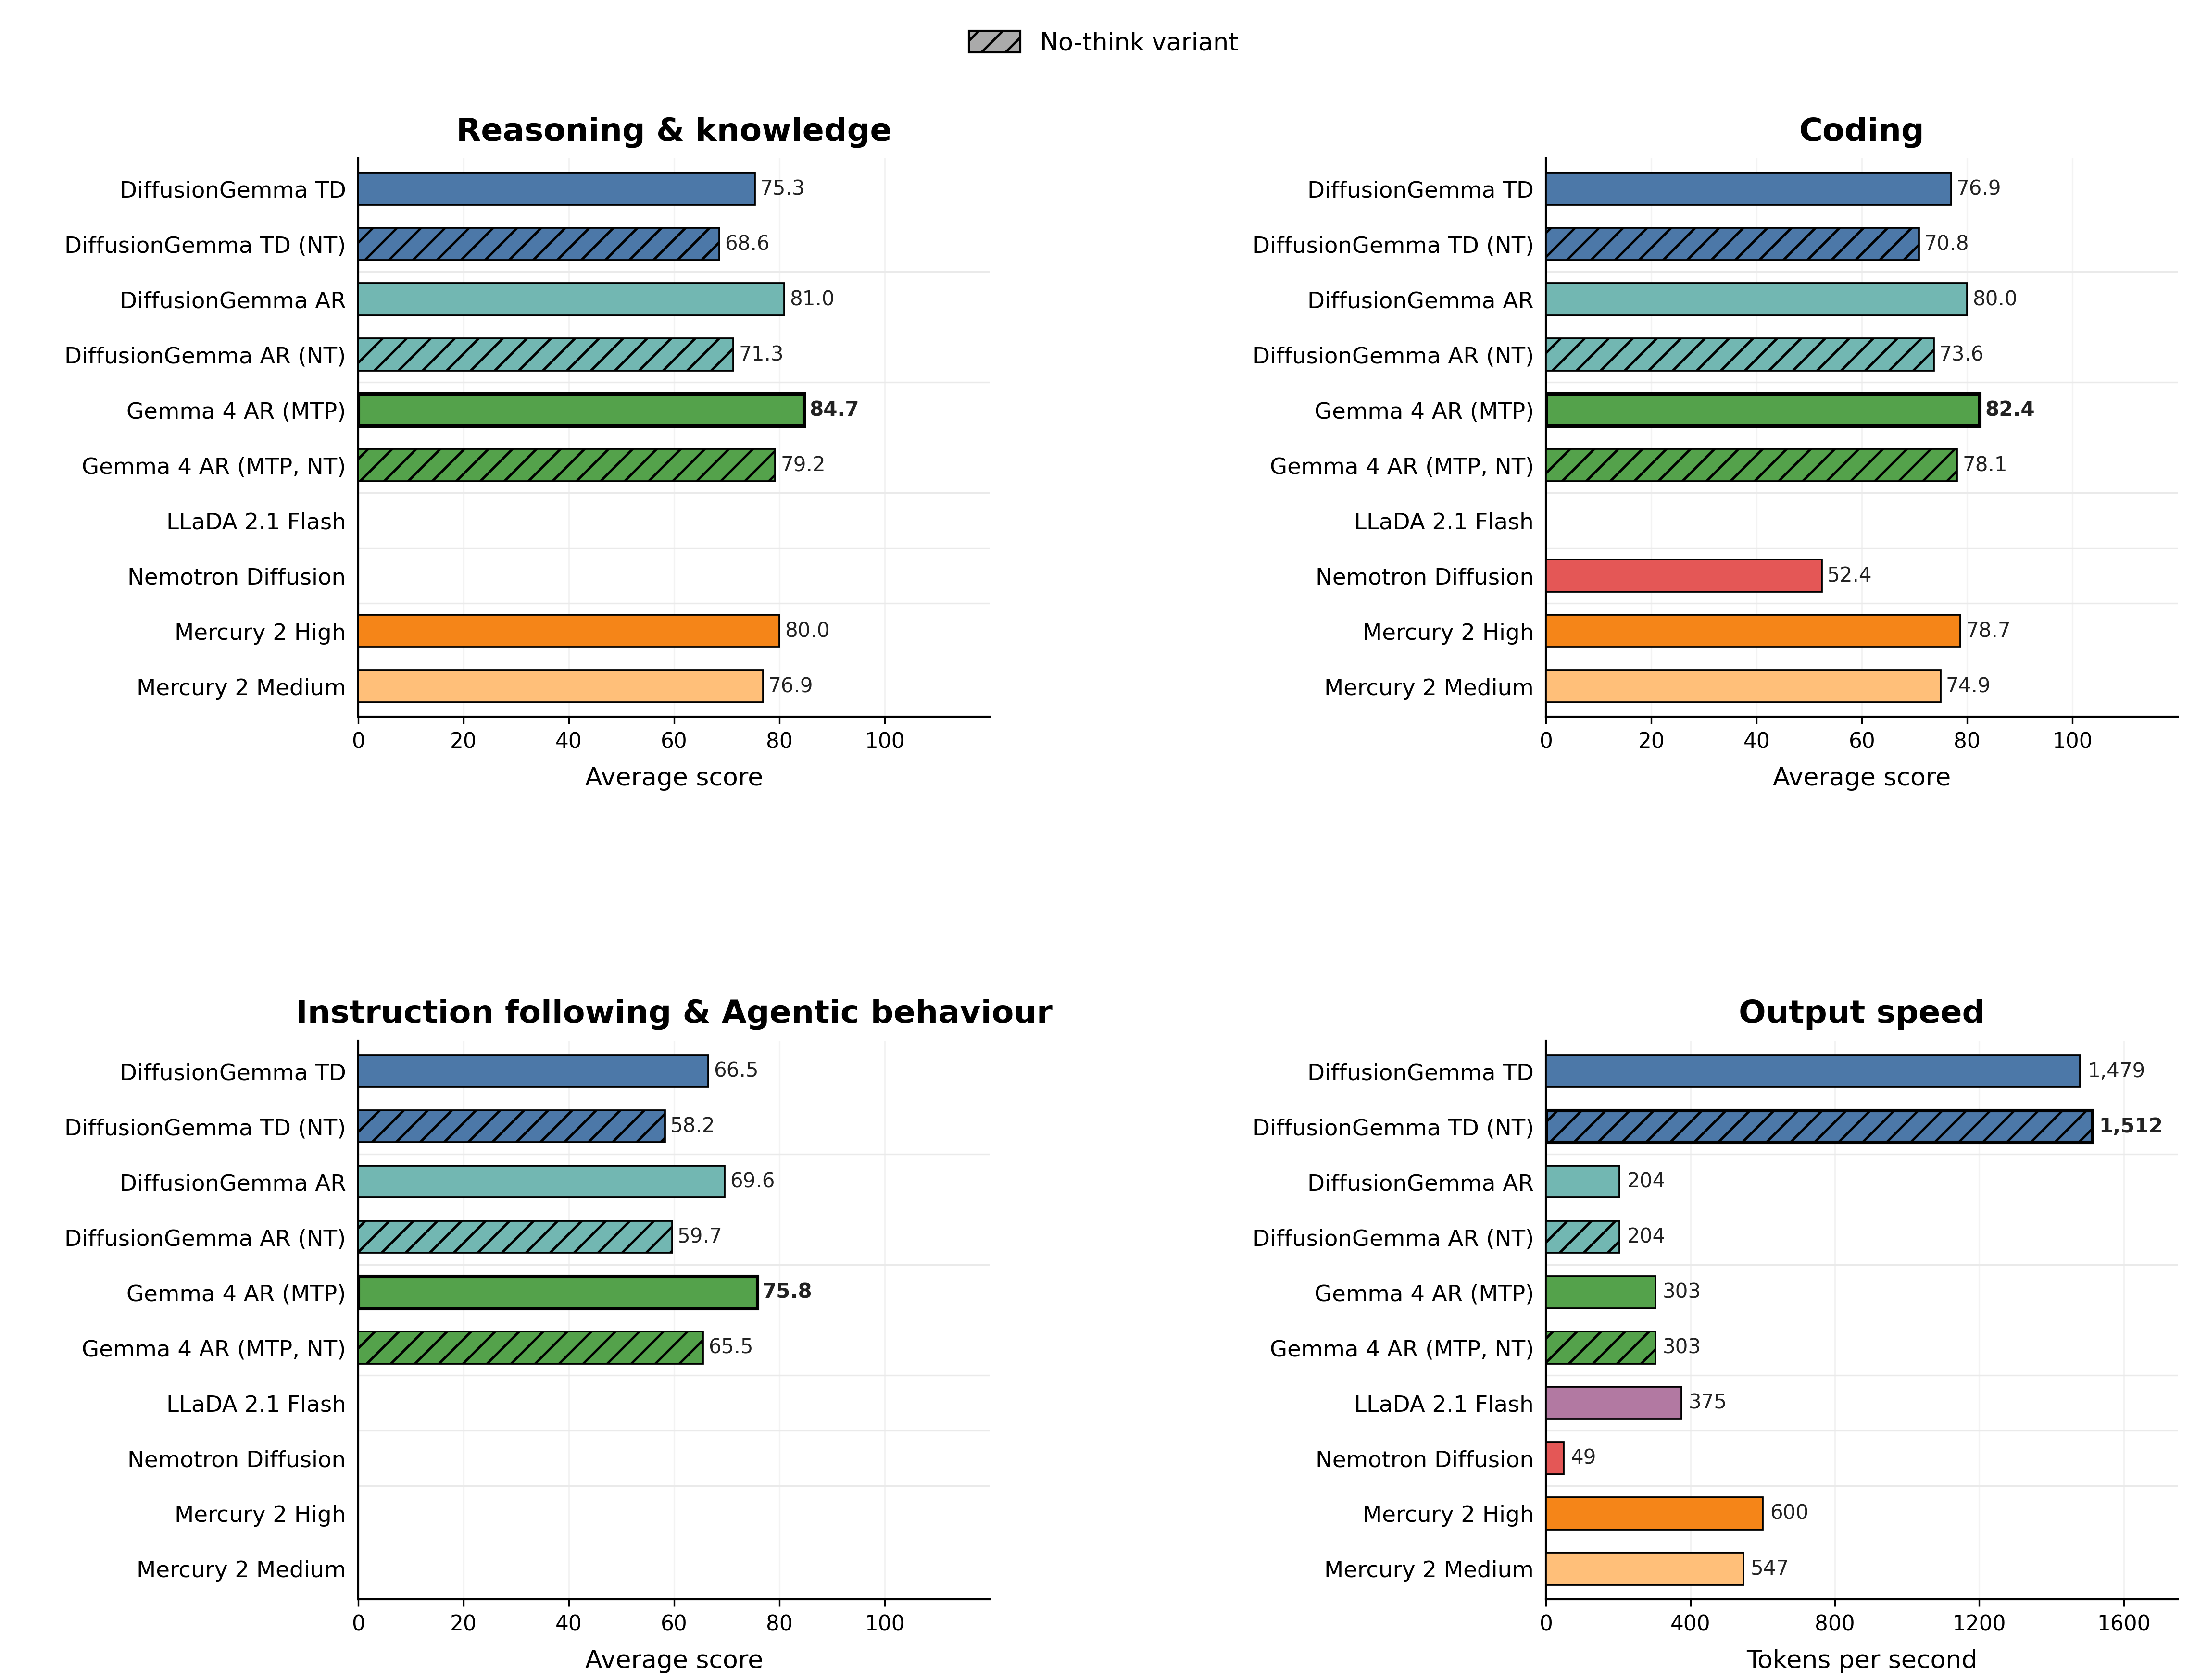
\includegraphics[
        width=\textwidth,
        height=0.70\textheight,
        keepaspectratio
    ]{assets/benchmark_summary_rev_b.png}
    \caption{
        \textbf{Capability 영역별 성능\textsuperscript{*}
        (해당 영역 0--100 점수의 비가중 평균)과 output 속도.} 완전한 커버리지가 없는 모델은 생략했다. non-thinking 변형은 줄무늬 막대로 표시한다. output 속도는 완전한 커버리지가 있는 7개 benchmark에서 평균한 값이며, Table~\ref{tab:model_comparison}을 참조하라.
    }
    \label{fig:benchmark_summary}
    \vspace{2pt}
    \parbox{\textwidth}{
        \footnotesize
        \raggedright
        \textsuperscript{*}
        Benchmark는 다음과 같이 묶었다:
        reasoning and knowledge
        (\textit{AIME 2026}, \textit{GPQA Diamond}, \textit{BigBench EH},
        \textit{GSM8K}, \textit{MGSM}, \textit{MMMLU}, \textit{Putnam},
        \textit{MMLU-Pro}, and \textit{HiddenMath});
        coding
        (\textit{LiveCodeBench V6}, \textit{HumanEval},
        \textit{BigCodeBench}, \textit{LBPP}, and \textit{Natural2Code});
        그리고 instruction following and agentic behaviour
        (\textit{IFEval}, \textit{Tau2 Retail}, \textit{Tau2 Airline},
        and \textit{Tau2 Telecom}).
    }
\end{figure*}

\begin{landscape} % Rotates the page orientation

%%%%%%%%%%% Quality metrics %%%%%%%%%%%%%%%%%%%
\definecolor{benchmarkhighlight}{RGB}{232,244,248} % subtle light blue
\begin{table}[t!]
\centering
\footnotesize
\setlength{\tabcolsep}{3pt}
\begin{tabular}{lcccccccccc}
\toprule
 & \multicolumn{8}{c}{\textbf{Open-weight 모델}} & \multicolumn{2}{c}{\textbf{Closed-weight 모델}} \\
\cmidrule(r){2-9} \cmidrule(l){10-11}
 & \multicolumn{4}{c}{DiffusionGemma} & \multicolumn{2}{c}{Gemma 4} & LLaDA 2.1 Flash & Nemotron Diffusion & \multicolumn{2}{c}{Mercury 2} \\
 & \multicolumn{4}{c}{26B A4B} & \multicolumn{2}{c}{26B A4B} & 100B & 14B & \multicolumn{2}{c}{Unknown} \\
\cmidrule(r){2-5} \cmidrule(r){6-7} \cmidrule(r){8-8} \cmidrule(r){9-9} \cmidrule(l){10-11}
모드 & TD & TD (No-think) & AR & AR (No-think) & AR (MTP) & AR (MTP, No-think) & TD (S Mode) & TD (Diffusion Mode) & High & Medium \\
\midrule
AIME 2026 & 69.1 & 50.8 & 84.2 & 57.5 & 88.3 & 80.0 & 80.0 & 40.0 & 91.7 & 82.5 \\
GPQA Diamond & 73.2 & 64.6 & 79.8 & 67.2 & 82.3 & 73.7 & 68.7 & 47.0 & 75.2 & 66.7 \\
LiveCodeBench-V6 & 69.1 & 60.6 & 71.4 & 58.3 & 77.1 & 72.6 & 39.4 & 28.6 & 79.4 & 74.9 \\
Codeforces ELO & 1429 & 959 & 1569 & 1059 & 1718 & 1529 & 718 & - & 1986 & 1629 \\
BigBench EH & 47.6 & 40.0 & 59.1 & 42.2 & 64.8 & 56.2 & - & - & 48.9 & 43.8 \\
GSM8K & 96.3 & 95.8 & 96.6 & 96.1 & 96.7 & 96.4 & 45.0 & - & 96.5 & 95.8 \\
MGSM & 84.8 & 80.7 & 87.9 & 84.3 & 92.9 & 91.5 & 6.8 & 69.3 & 91.9 & 91.2 \\
MMMLU & 81.5 & 76.3 & 82.2 & 78.0 & 86.3 & 78.0 & - & - & 81.9 & 80.6 \\
MMMU Pro & 54.3 & 66.0 & 63.3 & 66.7 & 73.8 & 72.5 & - & - & - & - \\
Putnam & 67.4 & 57.1 & 74.7 & 59.7 & 81.0 & 72.9 & - & 45.8 & 73.6 & 73.6 \\
HumanEval & 94.5 & 92.7 & 98.2 & 97.6 & 98.8 & 97.6 & 90.2 & 86.0 & 98.2 & 98.2 \\
BigCodeBench & 46.0 & 41.9 & 47.7 & 45.9 & 50.2 & 48.1 & - & 33.5 & 47.6 & 45.3 \\
LBPP & 81.0 & 68.9 & 86.3 & 74.1 & 89.5 & 77.3 & 45.7 & 40.7 & 89.2 & 85.0 \\
IFEval & 97.4 & 94.5 & 97.2 & 95.7 & 98.7 & 97.8 & - & 72.1 & 97.0 & 94.5 \\
Tau2 Retail & 71.5 & 57.5 & 75.4 & 61.0 & 85.5 & 79.0 & - & - & - & - \\
Tau2 Airline & 69.0 & 49.0 & 72.0 & 50.0 & 76.0 & 51.0 & - & - & - & - \\
Tau2 Telecom & 28.1 & 32.0 & 33.8 & 32.0 & 43.0 & 34.2 & - & - & - & - \\
MMLU-Pro & 77.6 & 77.9 & 78.8 & 79.1 & 82.6 & 82.6 & - & - & 77.6 & 75.5 \\
\rowcolor{benchmarkhighlight}
Natural2Code & 94.0 & 90.1 & 96.2 & 92.3 & 96.3 & 94.7 & 86.9 & 73.3 & 79.1 & 71.3 \\
\rowcolor{benchmarkhighlight}
HiddenMath & 80.6 & 74.3 & 85.4 & 77.5 & 87.2 & 81.6 & - & 44.3 & 82.7 & 82.3 \\
\midrule
출력 속도 (TPS) & 1479 & 1512 & 204 & 204 & 303 & 303 & 375 & 49 & 600 & 547 \\
Tokens Per Forward (TPF) & 19.74 & 18.76 & 1.00 & 1.00 & 1.40 & 1.40 & 4.63 & 1.79 & - & - \\
평균 전체 Token 수 & 4,001 & 829 & 5,184 & 1,025 & 7,207 & 1,816 & 4,371 & 941 & 3,882 & 1,222 \\
\bottomrule
\end{tabular}
\caption{\textbf{다양한 benchmark에서의 모델 성능, TPS, TPF 비교.} TPS는 prefill 시간을 제외하며, ``$-$''는 누락된 데이터를 뜻한다. 속도 측정은 다음과 같이 수행했다. DiffusionGemma와 Gemma~4는 1$\times$~H100(FP8, batch size~1), Nemotron~14B는 1$\times$~H100(bfloat16, batch size~1), LLaDA~2.1 Flash~100B는 8$\times$~B200(bfloat16, batch size~1), Mercury~2는 공개 API를 사용했다(속도 추정은 Appendix~\ref{sec:competitor-eval-methodology} 참조). TPS, TPF, 전체 token 수는 완전한 커버리지가 있는 7개 benchmark(AIME 2026, GPQA Diamond, LiveCodeBench-v6, MGSM, HumanEval, LBPP, Natural2Code)에서 평균했다. Gemma 4 (MTP)의 TPS와 TPF는 SPEED-Bench~\citep{abramovich2026speed}를 사용해 측정했다. Natural2Code와 HiddenMath 행은 proprietary, unleaked eval이므로 강조 표시했다.
}
\label{tab:model_comparison}
\end{table}

%%%%%%%%%%% Latency metrics %%%%%%%%%%%%%%%%%%%
\begin{table}[t!]
\centering
\small
\setlength{\tabcolsep}{2.5pt}
\begin{tabular}{l|cc|cc|cc|cc|cc|cc|cc}
\toprule
 & \multicolumn{2}{c}{\textbf{점수} ($\uparrow$)} & \multicolumn{2}{c}{\textbf{TPF} ($\uparrow$)} & \multicolumn{2}{c}{\textbf{TPS} ($\uparrow$)} & \multicolumn{2}{c}{\textbf{Effective DNS} ($\downarrow$)} & \multicolumn{2}{c}{\textbf{전체 Forward 수} ($\downarrow$)} & \multicolumn{2}{c}{\textbf{전체 Token 수}} & \multicolumn{2}{c}{\textbf{E2E 시간 (s)} ($\downarrow$)} \\
\cmidrule(lr){2-3} \cmidrule(lr){4-5} \cmidrule(lr){6-7} \cmidrule(lr){8-9} \cmidrule(lr){10-11} \cmidrule(lr){12-13} \cmidrule(lr){14-15}
\textbf{Benchmark} & \textbf{Think} & \textbf{No-Think} & \textbf{Think} & \textbf{No-Think} & \textbf{Think} & \textbf{No-Think} & \textbf{Think} & \textbf{No-Think} & \textbf{Think} & \textbf{No-Think} & \textbf{Think} & \textbf{No-Think} & \textbf{Think} & \textbf{No-Think} \\
\midrule
AIME 2026 & 69.1 & 50.8 & 19.3 & 16.7 & 1365.4 & 1333.0 & 12.6 & 14.1 & 390.6 & 91.1 & 6,445 & 1,309 & 4.72 & 0.98 \\
GPQA Diamond & 73.2 & 64.6 & 16.7 & 16.5 & 1207.8 & 1330.2 & 15.1 & 13.4 & 443.4 & 48.1 & 5,647 & 726 & 4.68 & 0.55 \\
LiveCodeBench-V6 & 69.1 & 60.6 & 18.5 & 16.9 & 1278.3 & 1333.4 & 13.8 & 14.0 & 581.8 & 195.7 & 7,534 & 1,847 & 5.89 & 1.39 \\
Codeforces ELO & 1429 & 959 & 15.1 & 14.0 & 950.5 & 1040.3 & 17.1 & 18.5 & 959.6 & 521.1 & 11,622 & 4,279 & 12.23 & 4.11 \\
BigBench EH & 47.6 & 40.0 & 20.8 & 17.7 & 1390.2 & 1415.1 & 11.9 & 12.8 & 434.9 & 68.1 & 9,062 & 1,233 & 6.52 & 0.87 \\
GSM8K & 96.3 & 95.8 & 23.2 & 24.1 & 1866.2 & 1966.4 & 9.1 & 7.5 & 43.4 & 13.2 & 883 & 298 & 0.47 & 0.15 \\
MGSM & 84.8 & 80.7 & 19.0 & 16.8 & 1526.7 & 1367.5 & 11.5 & 11.9 & 63.6 & 19.5 & 1,085 & 291 & 0.71 & 0.21 \\
MMMU Pro & 54.3 & 66.0 & 17.7 & 15.4 & 1351.3 & 1255.1 & 13.8 & 15.3 & 191.6 & 31.6 & 3,178 & 472 & 2.35 & 0.38 \\
Putnam & 67.4 & 57.1 & 18.1 & 16.0 & 1330.8 & 1282.4 & 13.4 & 14.4 & 303.8 & 77.4 & 4,725 & 1,103 & 3.55 & 0.86 \\
HumanEval & 94.5 & 92.7 & 23.0 & 24.3 & 1838.2 & 1981.2 & 9.4 & 8.0 & 55.6 & 14.3 & 1,174 & 305 & 0.64 & 0.15 \\
BigCodeBench & 46.0 & 41.9 & 19.6 & 19.4 & 1560.1 & 1579.0 & 11.3 & 10.1 & 77.3 & 21.8 & 1,410 & 394 & 0.90 & 0.25 \\
LBPP & 81.0 & 68.9 & 20.5 & 19.2 & 1509.8 & 1545.4 & 11.6 & 10.9 & 264.3 & 79.4 & 4,730 & 859 & 3.13 & 0.56 \\
IFEval & 97.4 & 94.5 & 17.2 & 9.0 & 1368.3 & 732.1 & 13.0 & 14.4 & 100.8 & 24.0 & 1,464 & 239 & 1.07 & 0.33 \\
Natural2Code & 94.0 & 90.1 & 21.1 & 21.0 & 1682.7 & 1706.5 & 10.5 & 9.6 & 70.5 & 24.7 & 1,391 & 465 & 0.83 & 0.27 \\
HiddenMath & 80.6 & 74.3 & 21.0 & 19.4 & 1591.2 & 1564.7 & 11.3 & 11.5 & 206.4 & 49.7 & 3,501 & 844 & 2.20 & 0.54 \\
\bottomrule
\end{tabular}
\caption{\textbf{Thinking 대 No-Thinking mode에서의 DiffusionGemma TD 성능 및 latency 지표.} 정확도/점수, Tokens Per Forward (TPF, 높을수록 빠름), Tokens Per Second (TPS), Effective Denoising Steps (DNS, 낮을수록 빠름), 전체 Forward 수, 전체 Token 수, 샘플당 End-to-End Latency(초, prefill 시간 제외)를 보고한다. latency 지표는 각 benchmark의 모든 샘플에 대해 평균했다.}
\label{tab:dg_td_latency}
\end{table}

\end{landscape}


\section{오픈소스 Downstream SFT}\label{sec:downstream_sft}

DiffusionGemma와 함께, 실무자가 자신의 domain-specific 데이터셋에 모델을 적응시킬 수 있도록 하는 오픈소스 finetuning toolkit도 공개한다. 이는 생성 모델링을 위한 모듈식 오픈소스 연구 툴박스인 Hackable Diffusion~\citep{hackable_diffusion2026github} 위에 구축했다.
또한 소비자용 하드웨어에서도 finetuning할 수 있도록 Low-Rank Adaptation (LoRA) recipe~\citep{hu2021loralowrankadaptationlarge}를 제공한다.

\paragraph{Finetuning procedure.} 우리의 오픈소스 SFT toolkit은 causal encoder objective와 diffusion decoder objective를 모두 포함한다. 학습 시퀀스의 길이는 $P+KC$이며, 여기서 $P$는 prompt token 수, $K$는 canvas 수, $C$는 canvas 크기다. 전체 loss를 계산하기 위해 encoder는 먼저 전체 시퀀스의 모든 token을 처리해 KV cache $H$를 채우고, encoder용 표준 cross-entropy loss에 들어갈 next token prediction을 제공한다. decoder loss는 사용 가능한 $K$개 canvas 중 하나 $k$를 균등하게 sampling하여 계산한다. canvas $k$에 대해 현재 noisy state $x_t$, prompt와 시퀀스 내 이전 canvas들(즉 canvas $1$, $2$, \ldots, $k-1$)에 대한 KV cache $H$, 그리고 decoder가 예측한 logits를 사용해 denoising cross-entropy loss를 평가한다. batch의 데이터포인트 중 $50\%$에 대해서는 decoder가 이전 forward pass에서 계산한 self-conditioning state $z_t$에도 조건화된다. 나머지 $50\%$는 $z_t = \textbf{0}$이다.
형식적으로 loss는 다음과 같이 쓴다
\begin{equation}
   L_{\text{encoder}}(\theta) = - \frac{1}{P+KC} \sum_{j=1}^{P+KC} \log p_\theta(x^j \mid x^{1:j-1}) , \quad  \quad L_{\text{decoder}}(\theta) = - \frac{1}{C} \sum_{i=1}^C \log p_\theta(x_0^{i} \mid x_t, z_t, H).
\end{equation}
encoder loss에서는 $j$가 시퀀스의 모든 token(prompt와 canvas)을 따라 인덱싱하고, decoder loss에서는 $i$가 주어진 canvas의 token을 따라 인덱싱한다. 최종 loss는 두 loss의 합이다.

\paragraph{LoRA for parameter-efficient finetuning.} LoRA는 모든 선형 연산(attention projection, MLP gate, MoE router, self-conditioning feedforward block)에 적용된다. 이를 통해 2$\times$ A100 80GB GPU만으로도 모델 파라미터의 작은 일부만 학습하면서 강한 downstream 성능을 달성할 수 있다. 학습 세부사항은 모두 Appendix~\ref{sec:sft-hd-appendix}에 보고한다.


\begin{figure}[tbp]
    \centering
    % --- LEFT SIDE: FIGURE MINIPAGE ---
    \begin{minipage}[b]{0.45\textwidth}
        \centering
        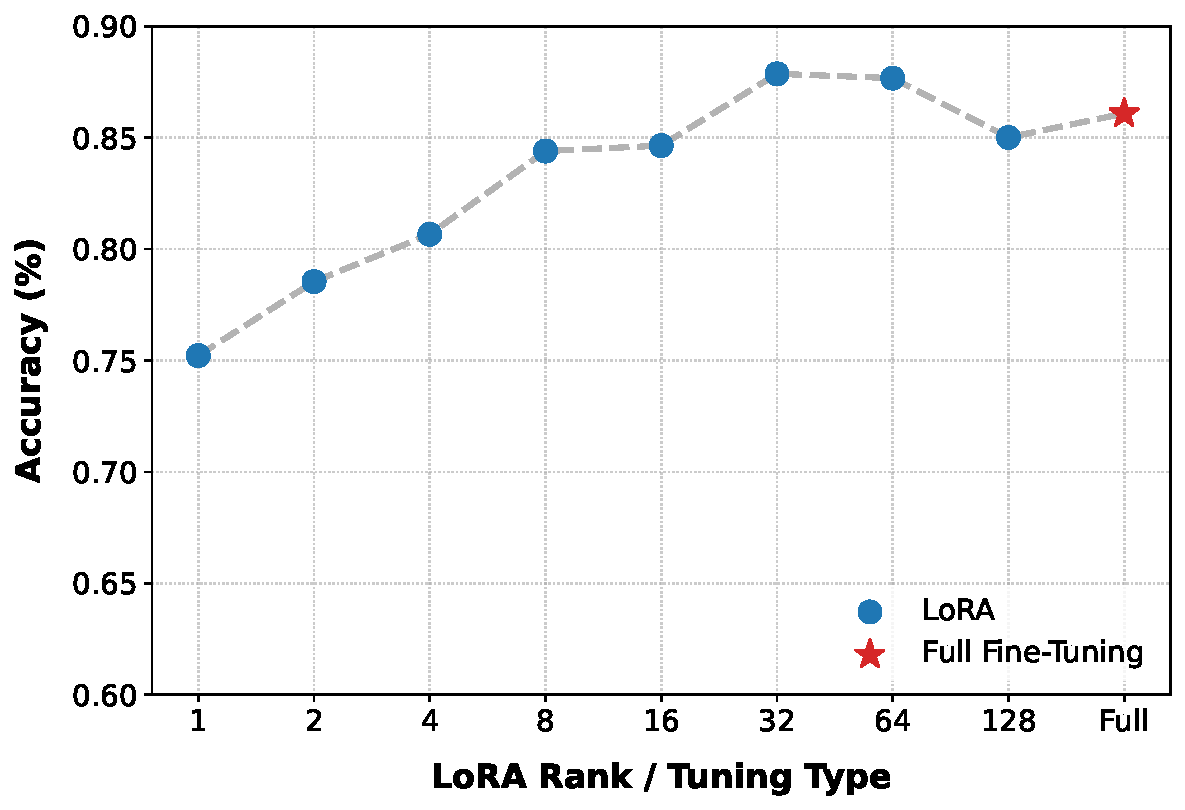
\includegraphics[width=\linewidth]{assets/downstream_sft_figures/lora_accuracy_comparison.pdf}
        \captionof{figure}{
            \textbf{Sudoku downstream SFT 성능.} x축은 LoRA rank이고 y축은 모델 정확도다.
        }
        \label{fig:sft-sudoku} 
    \end{minipage}
    \hfill % Inserts elastic horizontal space to push them to the outer edges
    % --- RIGHT SIDE: TABLE MINIPAGE ---
    \begin{minipage}[b]{0.50\textwidth}
        \centering
        \vspace{5pt} % Adds professional spacing between the caption and the table top rule
        \small % Slightly reduces font size if needed to fit perfectly beside the figure
        \begin{tabular}{lcc}
        \toprule
        모델 & Denoising Step 수 & 정확도 (\%)  \\
        \midrule
        DiffusionGemma & 40.65 & 0.00 \\
        + LoRA finetuning & \textbf{10.72} & \textbf{84.40} \\
        \bottomrule
        \end{tabular}
        \captionof{table}{\textbf{LoRA rank 8로 finetuning한 모델의 Sudoku 정확도.}
        기반 모델은 finetuning 이전에는 올바른 Sudoku grid를 생성하지 못한다. finetuning 후에는 더 낮은 predictive entropy 덕분에 훨씬 적은 effective denoising step을 사용하면서도 정확도가 $80\%$를 넘는다.}
        \label{tab:sudoku_steps_vs_acc}
    \end{minipage}
\end{figure}


\paragraph{Case study: Sudoku puzzle solving.} Sudoku 퍼즐 풀기는 작업 자체가 non-autoregressive하다는 점에서 discrete diffusion의 매력적인 testbed다. 우리는 DiffusionGemma를 Sudoku 퍼즐 오픈소스 데이터셋으로 finetuning했다.\footnote{\url{https://www.kaggle.com/datasets/rohanrao/sudoku}} full finetuning을 적용하면 sampler(Algorithm~\ref{alg:sampling})는 $4096$개 held-out 퍼즐 집합에서 퍼즐 단위 정확도 $85\%$ 이상을 달성한다(Figure~\ref{fig:sft-sudoku}). LoRA rank를 낮추면 정확도와 compute 사이의 절충이 생긴다. Table~\ref{tab:sudoku_steps_vs_acc}에는 원래 모델과 finetuned 모델의 성능을 함께 보고한다. PubMedQA~\citep{jin2019pubmedqa}에 대한 추가 결과는 Appendix~\ref{sec:sft-hd-appendix}를 참조하라.



\section{Text Diffusion의 실용적 장점}\label{sec:advantages}

이 원고에서는 text diffusion이 표준 AR language modeling보다 갖는 주된 장점으로 저지연을 주로 강조해 왔다 \citep{ghazvininejad2019mask, gong2022diffuseq, li2022diffusionlm, dieleman2022continuous}. 그러나 text diffusion의 아키텍처 패러다임은 계산 효율을 넘어서는 여러 이점을 제공한다. 여기서는 모델이 생성한 샘플의 구체적 예시와 정성적 분석을 통해 그 실질적 장점을 보여 준다. 아키텍처 자체의 고유 능력을 분리해 보기 위해, DiffusionGemma와 기준 Gemma AR 모델 모두에서 명시적 thinking mode를 비활성화한다. 이를 통해 기반 생성 과정 자체를 관찰하고 평가할 수 있다.


\subsection{양방향 추론과 자기 수정}
AR next-token prediction은 본질적으로 causal하다. 어떤 token을 생성하는 동안 모델은 앞선 context에만 attention할 수 있다. 아직 생성되지 않은 token에 조건화할 능력이 근본적으로 없다. 반면 text diffusion은 canvas 전반에 걸친 완전한 bidirectional attention으로 작동한다. 이 non-causal 특성 덕분에 canvas의 임의 위치에 있는 token이 과거와 미래 표현 모두에 동시에 attention할 수 있으며, 이는 초기 결정이 최종 결과에 의존하는 복잡한 계획 및 reasoning 작업에서 핵심적인 능력이다 \citep[e.g.,][]{papadopoulos2024arrows, kitouni2024factorization, zhangli2024reverse, nagarajan2025roll}. 따라서 canvas 내부의 국소 영역에서는 미래 token이 더 이른 token 형성에 직접 영향을 줄 수 있다.

text diffusion은 반복 정제 과정을 사용하기 때문에, self-correction을 위한 내장 메커니즘을 갖고 있다. 더 이른 denoising step에서 이루어진 성급한 확정은 이후 denoising 반복에서 수정될 수 있다 \citep{reid2022diffuser, han2023ssdlm}. 우리는 이미 Sudoku 같은 구조화된 논리 퍼즐에서 bidirectional reasoning과 self-correction의 효용을 보여 준 바 있지만, 여기서는 이 메커니즘을 두 개의 reasoning 예시로 다시 보여 준다.

Figure \ref{fig:math_reasoning}에 제시한 다단계 산술 문제를 보자. causal 생성에 묶인 AR Gemma 모델은 중간 계산을 서술하기 전에 최종 답의 첫 token을 먼저 확정해야 한다. 이 때문에 모델은 나중에 다시 고쳐야 하는 잘못된 초기 예측($-1$)을 내놓게 된다. 반대로 DiffusionGemma는 bidirectional attention canvas를 활용해 최종 답과 그 근거 논리를 동시에 발전시킨다. 함께 제시한 denoising trace에서 보이듯, 병렬 diffusion 과정은 잘못된 중간 상태를 탐색하기도 하지만 새로 형성되는 reasoning token을 이용해 방향을 수정하며 올바른 답($-25$)으로 자연스럽게 수렴한다. bidirectional attention과 denoising을 통한 논리적 reasoning 및 수정의 두 번째 예시는 Appendix~\ref{app:advantages_bidir}를 참조하라.

\begin{figure}[htbp]
\begin{tcolorbox}[
  colback=gray!5,
  colframe=gray!50,
  fontupper=\small,
  title={\sffamily\bfseries Prompt}
]
``Solve $7 \times (\sqrt{111 + 10} - 3) - 9^2$. Give the answer first
then provide the reasoning, be concise.''

\medskip
\begin{tcolorbox}[colback=red!3, colframe=red!25, boxrule=0.4pt, left=4pt, right=4pt]
\textbf{Gemma~4 26B A4B:}
$-1$

\textbf{Reasoning:}
\begin{enumerate}[nosep, leftmargin=1.5em]
  \item Inside parentheses: $111 + 10 = 121$.
  \item Square root: $\sqrt{121} = 11$.
  \item Inside parentheses continued: $11 - 3 = 8$.
  \item Multiplication: $7 \times 8 = 56$.
  \item Exponent: $9^2 = 81$.
  \item Subtraction: $56 - 81 = -25$.
\end{enumerate}
Correction: Wait, recalculating: $56 - 81 = -25$.

Correct Answer: $-25$
\end{tcolorbox}

\smallskip
\begin{tcolorbox}[colback=green!3, colframe=green!30, boxrule=0.4pt, left=4pt, right=4pt]
\textbf{DiffusionGemma:}
$-25$

\textbf{Reasoning:}
\begin{enumerate}[nosep, leftmargin=1.5em]
  \item Simplify inside the square root: $\sqrt{111 + 10} = \sqrt{121} = 11$.
  \item Solve inside the parentheses: $(11 - 3) = 8$.
  \item Multiply: $7 \times 8 = 56$.
  \item Calculate the exponent: $9^2 = 81$.
  \item Final subtraction: $56 - 81 = -25$.
\end{enumerate}
\end{tcolorbox}

\smallskip
{\footnotesize \textbf{Analysis:} Constrained by causal generation, Gemma~4 commits to the incorrect answer ``$-1$'' in its very first tokens. As it autoregressively generates its reasoning, it discovers its own error and is forced to append a correction. Conversely, DiffusionGemma produces the correct answer ``$-25$'' immediately, preventing logical contradictions. Note that both models are operating in non-thinking mode.}
\end{tcolorbox}

\vspace{1em}
\centering
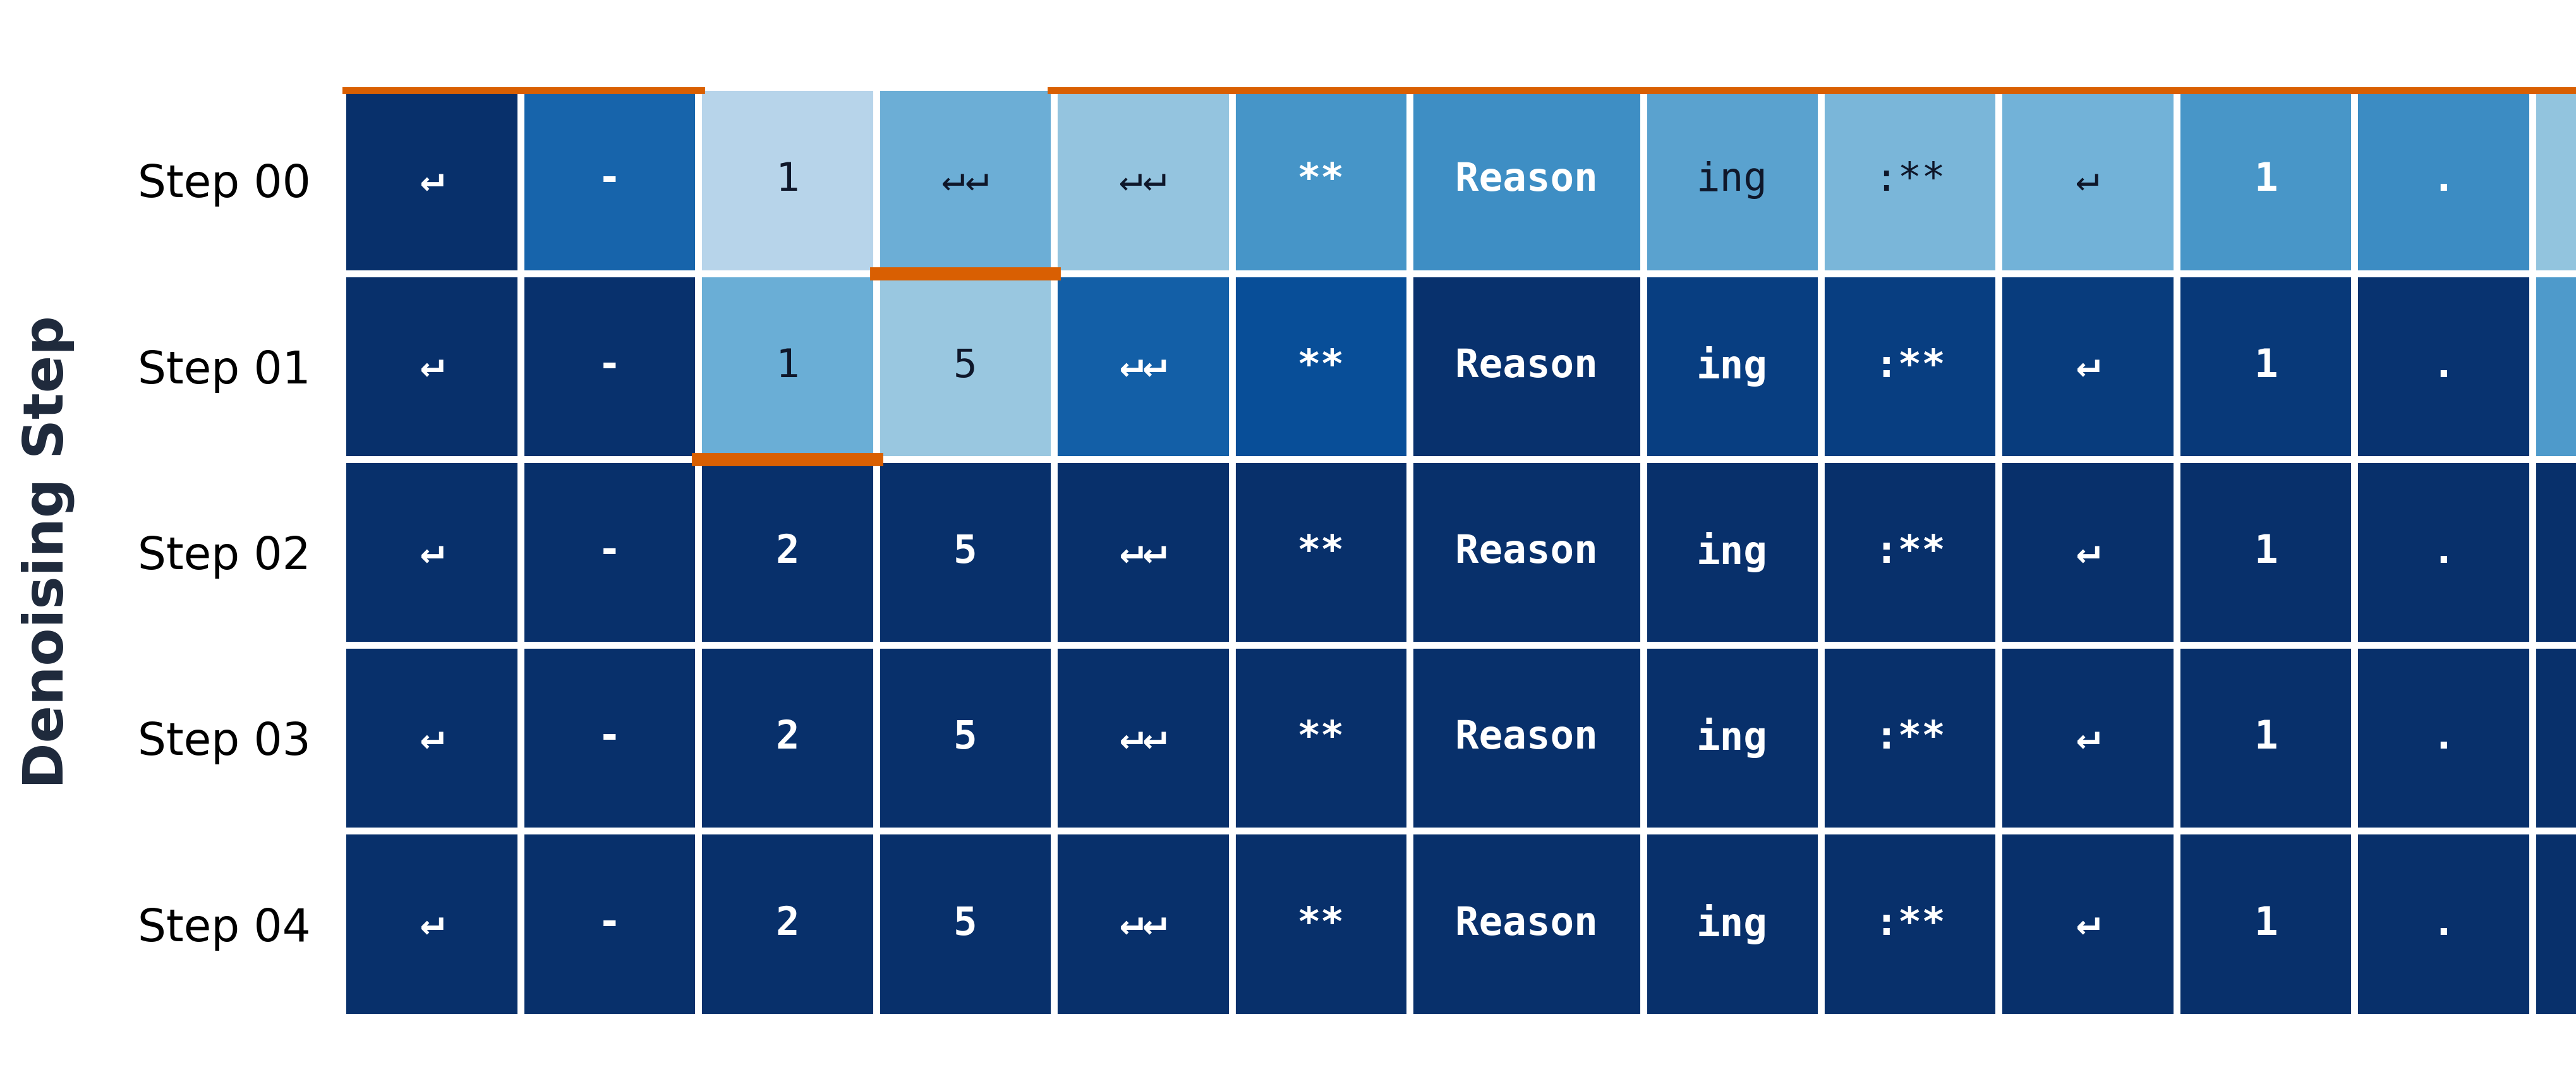
\includegraphics[clip, viewport=0bp 0bp 500bp 230bp, width=0.9 \linewidth]{assets/td_reasoning_cropped.png}
\caption{\textbf{Denoising trace for the math reasoning problem (zoomed in to the first 12 tokens), where color intensity indicates model confidence}. DiffusionGemma initially makes the same causal estimation mistake as the AR model, assigning high probability to $-1$. However, through iterative bidirectional refinement, it suggests $-15$ in the next step before fully converging to the correct answer $-25$. The parallel denoising process allows the final answer and reasoning steps to inform one another. Denoising is completed in just 5 steps.}
\label{fig:math_reasoning}
\end{figure}

\subsection{동적이고 적응적인 계산}

생성 token마다 본질적으로 고정된 양의 계산을 할당하는 AR 모델과 달리, text diffusion은 동적인 test-time compute를 가능하게 한다. text diffusion 모델은 주어진 prompt에 투입할 계산량을 자율적으로 조절할 수 있으며, 작업 고유의 난이도에 따라 더 긴 inference 시간을 더 나은 생성 성능과 맞바꿀 수 있다 \citep{ye2024diffusion}. DiffusionGemma는 adaptive stopping을 통해 작업 난이도에 자동으로 적응한다. Figure~\ref{fig:boxplot_evals_effective_denoising_steps}에서 보이듯, 복잡도가 서로 다른 작업은 자연스럽게 서로 다른 수의 effective denoising step을 유도한다. 이는 쉬운 질의에서는 compute를 아끼고 복잡한 reasoning에는 더 많은 compute를 쓰게 해 준다. Appendix~\ref{app:advantages_adaptive}에서는 구조적으로 ``어려운'' 생성 작업과 구조적으로 ``쉬운'' 작업을 대비시켜 text diffusion의 적응적 행동을 구체적으로 보여 주며, 쉬운 작업이 더 적은 denoising step을 필요로 한다는 점과 두 경우에 token canvas를 따라 정보가 서로 다르게 전파된다는 점을 함께 보인다.

또한 denoising step의 최대 개수는 latency-품질 절충을 관리하는 명시적 설정 파라미터 역할을 한다. step 수가 적으면 모델은 역과정을 더 거칠게 통과하게 되어 더 빠른 결과를 얻는 대신 출력 정밀도는 낮아진다. step 수를 늘리면 생성 과정의 해상도가 더 세밀해져 품질은 극대화되지만 필요한 compute 시간도 길어진다. Figure~\ref{fig:score_vs_dns}는 이 연속적 관계를 나타내며, 다양한 운영 제약에 맞게 모델을 동적으로 조정할 수 있음을 보여 준다.

\subsection{구조화되고 제약된 출력}
많은 실용적 애플리케이션에서 원하는 출력은 엄격하고 고도로 구조화된 형식(예: JSON schema)을 따르거나, optical character recognition (OCR), code editing, 세밀한 구문 제어처럼 입력 prompt에 강한 어휘적 의존성을 보인다 \citep{chen2023textdiffuser, li2022diffusionlm}. text diffusion은 모든 token을 병렬로 생성하고 정제하기 때문에, 이러한 구조적 prior를 자연스럽게 활용해 수렴을 가속한다. AR 모델은 이런 능력이 없다. 엄격한 순차 디코딩에 묶여 있기 때문에, token이 고정된 boilerplate이거나 입력 context의 축어적 복사본이더라도 $N$개의 token을 생성하려면 똑같이 $O(N)$ 계산 비용을 치러야 한다. 반면 DiffusionGemma는 전체 시퀀스에 걸친 예측 가능한 구문 구조를 동시에 식별하고 고정할 수 있다. 우리는 이 효율을 두 가지 현실적 예시로 보여 준다. 엄격한 JSON 추출(Appendix~\ref{app:advantages_structure}, Figures \ref{fig:json-prompt}와 \ref{fig:json-denoising})과 Python 코드 디버깅(Appendix~\ref{app:advantages_structure}, Figures \ref{fig:python-prompt}와 \ref{fig:bug-fix})이다. 두 경우 모두 강하게 제약된 출력 덕분에 diffusion 과정이 단 2-3 step 만에 수렴하며, 순차 디코딩 대비 latency가 크게 줄어듦을 분명히 보여 준다.

\section{한계와 알려진 이슈} \label{sec:limitations}

이전 절에서는 text diffusion의 새로운 emergent property와 AR language modeling 대비 우리의 접근이 갖는 장점을 논의했다. DiffusionGemma는 생성 텍스트 모델링과 inference 효율에서 새로운 Pareto frontier를 세우지만, 현재의 실험적 공개 버전에는 다음과 같은 알려진 한계가 있다:


\begin{itemize}[topsep=0pt]

    \item \textbf{AR baseline 대비 성능 격차:} AR 초기화 모델(Gemma 4 26B A4B)보다 절대 성능이 낮은 이유는 여러 실용적 제약 때문이다. native diffusion pretraining을 건너뛰고 AR 가중치에서 warm-start한 점, compute budget 제약으로 인해 비교적 짧은 SFT 단계에 의존한 점, 초저지연을 명시적으로 목표로 하여 점근적 성능과 본질적인 절충을 하는 온라인 학습 알고리즘(\sdrl)을 사용한 점, 그리고 discrete diffusion 패러다임에는 최적이 아닐 수 있는 아키텍처·최적화·데이터 혼합 결정을 AR baseline으로부터 물려받은 점이 모두 영향을 준다.

    \item \textbf{생성 길이와 간결성:} Section~\ref{sec:sdrl}에서 언급했듯, 최종 checkpoint는 매우 간결한 출력을 생성한다. 이러한 emergent한 짧음은 inference 속도를 키우는 배수 효과를 주지만, 더 길고 정교한 reasoning trace가 보통 가져오는 품질 향상을 모델이 활용하지 못하게 한다.

    \item \textbf{간헐적인 token stuttering:} 드물게 모델 출력이 반복 loop나 국소적 stuttering(예: ``the the the'' 같은 흔한 token을 끝없이 반복함)으로 퇴화한다. \sdrl 학습이 대다수 사례를 성공적으로 완화했지만, 이 드문 artifact는 공격적으로 denoising step 수를 줄인 초저지연 regime에서 작동한다는 사실의 직접적인 결과이며, 때때로 생성 과정의 강건성이 손상될 수 있다.
    
    \item \textbf{멀티모달 작업에서 closing thought tag가 가끔 누락됨:} multimodal prompt를 처리할 때, 모델은 reasoning이 올바른 경우에도 closing thought tag를 항상 안정적으로 생성하지는 않는다. 이는 특정 benchmark의 thinking mode 성능을 인위적으로 끌어내릴 수 있다. 예를 들어 MMMU-Pro에서는 thinking 점수가 non-thinking 점수보다 낮다(54.3 vs.\ 66.0). 이 문제는 이번 공개 버전에 수정을 적용하기에는 파이프라인에서 너무 늦게 발견되었다.

    \item \textbf{큰 batch size에서의 처리량 한계:} DiffusionGemma는 memory-bandwidth 비용을 compute로 바꾸는 방식으로 low batch size에서 뛰어난 성능을 보이며, 최대 약 $\sim$32명의 동시 사용자까지는 사용자당 및 총 처리량 모두에서 Gemma~4~AR(MTP 포함)을 능가한다(Figure~\ref{fig:inference-throughput}). 이 지점을 넘어서면 token당 compute 비용이 더 높기 때문에 AR 모델이 처리량 우위를 얻게 된다. Section~\ref{sec:inference_optimizations}에서 언급했듯, 이 결과는 batch-size 표적 최적화 없이 얻은 것이며, 현실적 트래픽 조건에서의 철저한 실증 분석은 향후 과제로 남아 있다.


\end{itemize}



\section{결론} \label{sec:conclusion}
DiffusionGemma는 초고속 텍스트 생성을 향한 실용적이고 compute-efficient한 경로를 보여 준다. 기존 Gemma 4 26B A4B AR 모델을 우리의 2단계 학습 파이프라인(SFT와 \sdrl)으로 finetuning해 text diffusion을 수행하게 함으로써, reasoning과 multimodal 능력을 매우 경쟁력 있게 유지하면서도 단일 H100에서 초당 약 1,500 token을 달성하는 속도-지능 절충의 새로운 Pareto frontier를 세운다. 우리는 HuggingFace Transformers와 vLLM의 참조 구현과 함께 DiffusionGemma를 실험적 open-weight 모델로 공개함으로써, 오픈소스 커뮤니티가 text diffusion의 경계를 넓혀 가도록 힘을 실어 주고자 한다. 연구자와 실무자가 이 접근을 바탕으로 특화 작업용 finetuning을 하거나, 새로운 sampling 알고리즘을 탐색하거나, inference 효율을 더 최적화하기를 기대한다.

\bibliography{main}

\newpage

\appendix

\phantomsection
\section*{기여자 및 감사의 말 (알파벳순)}
\label{sec:contributions}

\noindent\textbf{핵심 기여자 (워크스트림 리드에는 ‘*’ 표시)}

\begin{multicols}{3}
\noindent
Adrien Ali Taïga \\ 
James Assiene \\ 
Daniele Calandriello* \\ 
Rahma Chaabouni \\ 
João Gante*  \\ 
Tamara von Glehn* \\ 
Nate Keating \\ 
Chris Knutsen \\ 
Martin Kukla* \\ 
Tianlin Liu \\ 
Ivan Lobov* \\ 
Ofir Nabati \\ 
João Gabriel Oliveira \\ 
Nicolas Perez-Nieves* \\ 
Nastasia Prutianova \\ 
Bobak Shahriari* \\ 
Jean Tarbouriech* \\ 
Pavel Tyletski \\ 
Çağlar Ünlü \\ 
Cindy Wu
\end{multicols}

\noindent\textbf{기여자}

\begin{multicols}{3}
\noindent
Glenn Cameron \\ 
Jerome Connor \\ 
Sertan Girgin \\ 
Maarten Grootendorst \\ 
Alon Levkovitch \\ 
Eliya Nachmani \\ 
Omar Sanseviero \\ 
Piotr Stanczyk
\end{multicols}

\noindent\textbf{Finetuning 프레임워크}

\begin{multicols}{3}
\noindent
Quentin Berthet \\ 
Andrew Campbell \\ 
Clément Crepy \\ 
Valentin De Bortoli \\ 
Arnaud Doucet \\ 
Romuald Elie \\ 
Alexandre Galashov \\ 
Klaus Greff \\ 
Alexis Jacq \\ 
David Ruhe \\ 
Yu-Han Wu
\end{multicols}

\noindent\textbf{리드}

\begin{multicols}{3}
\noindent
Sebastian Flennerhag \\ 
Brendan O'Donoghue \\ 
George Scrivener \\ 
Shantanu Thakoor
\end{multicols}

\noindent\textbf{감사의 말}

\begin{multicols}{3}
\noindent
Sander Dieleman \\
Lucas Dixon \\
Johan Ferret \\
Parnian Kassraie \\
Preethi Lahoti \\
Gaël Liu \\
Sarah Perrin \\
Angéline Pouget \\
Louis Rouillard \\
Pier Giuseppe Sessa \\
Danilla Sinopalnikov \\
Gemma Team \\
\end{multicols}

\noindent\textbf{후원자}

\begin{multicols}{3}
\noindent
Olivier Bachem \\ 
Jeff Dean \\ 
Zoubin Ghahramani \\ 
Raia Hadsell \\ 
Demis Hassabis \\ 
Prateek Jain \\ 
Armand Joulin \\ 
Koray Kavukcuoglu \\ 
Marc’Aurelio Ranzato \\ 
Oriol Vinyals
\end{multicols}


\newpage

\section{관련 연구} \label{sec:related_work}

\subsection{텍스트를 위한 Continuous Diffusion}

Discrete diffusion이 여전히 매우 효과적이긴 하지만, 최근의 진전은 continuous 및 hybrid 접근의 부활을 시사한다. Embedded Language Flows 같은 flow-matching 프레임워크는 step별 token supervision을 버리고 최종 discretization step까지 제약 없는 continuous embedding 공간에 머무름으로써, continuous 모델이 discrete baseline을 크게 능가할 수 있음을 보여 주었다 \citep{hu2026elf}. 이 continuous 패러다임 위에서, discrete data를 위한 flow map의 최근 진전은 학습 동학을 probability simplex의 기하와 정렬함으로써 이러한 생성 trajectory를 single-step mapping으로 압축해 한두 step 만에 고품질 병렬 언어 생성을 달성할 수 있음을 보였다 \citep{lee2026flowmap, potaptchik2026discrete}. 유사하게, 사전학습된 contextual autoencoder(예: Cosmos, TEncDM)를 사용하는 모델은 텍스트를 압축되고 매끄러운 latent 공간으로 사상하는데, 여기서는 Gaussian diffusion이 rounding error 없이 효율적으로 작동하며, 고급 guidance 기법에 적합한 continuous manifold를 제공한다 \citep{he2024manifold, meshchaninov2025cosmos, shabalin2025tencdm}. 한편 hyperspherical flow 같은 최근 접근은 token embedding을 초구면 위에서 회전시켜 언어의 기하 구조와 더 잘 맞추는 방식으로 Gaussian corruption을 피한다 \citep{deschenaux2026hyperspherical}. CANDI \citep{pynadath2025candi} 같은 다른 hybrid 프레임워크는 discrete data에 Gaussian noise를 적용할 때의 ``temporal dissonance''를 discrete corruption과 continuous corruption의 분리로 해결하여, 모델이 조건부 구조와 연속 기하를 동시에 학습하게 한다. 동시에 Score Entropy Discrete Diffusion은 continuous-time Markov chain을 적용해 discrete data 분포의 확률 비를 학습함으로써 이 영역들을 연결했다 \citep{lou2024discrete}. 이러한 돌파구는 continuous text diffusion의 초기 실패가 본질적 모달리티 한계라기보다, 비최적의 공간 기하와 제한적인 학습 목적함수의 산물이었을 수 있음을 시사한다.

\subsection{Speculative Decoding}

Speculative decoding~\citep{leviathan2023fast,chen2023accelerating,xia-etal-2024-unlocking}은 더 작은 draft 모델이 token 시퀀스를 제안하고 이를 더 큰 target 모델이 병렬 검증하게 함으로써 serving latency를 줄인다. 전체 latency는 draft 모델과 target 모델 양쪽의 생성 시간에 모두 좌우된다. AR drafter~\citep{li2026eagle}는 순차 생성에 근본적으로 제약된다. draft 품질을 높이려면 더 많은 파라미터가 필요하고, 이는 token당 latency를 늘려 end-to-end 이득을 약화시킨다. Medusa~\citep{cai2024medusa} 같은 병렬 drafter는 한 번에 많은 token을 생성함으로써 이를 우회하지만, token을 독립적으로 생성하기 때문에 acceptance rate가 최적보다 낮다. diffusion 기반 drafter는 대신 draft token의 결합분포를 모델링함으로써 token 간 의존성을 복원한다. TiDAR~\citep{liu2025tidar}는 diffusion 기반 drafting과 AR verification에 단일 모델을 사용하며, 이는 DiffusionGemma도 지원하는 구성이다. 반면 DFlash~\citep{chen2026dflash}는 별도 모델을 drafter로 사용한다. 그러나 이 방식은 suffix decay를 보여, 뒤쪽 draft 위치로 갈수록 acceptance rate가 낮아진다~\citep{cheng2026dspark}. DSpark~\citep{cheng2026dspark}는 병렬 backbone 위에 가벼운 AR module을 추가해 이를 해결한다. 이와 달리 DiffusionGemma는 독립형 diffusion 모델로 작동하여 verification 병목을 제거하고, draft-then-verify 접근보다 더 긴 생성 canvas로 확장된다.





\section{\texorpdfstring{\sdrl}{} 학습 전후 샘플}\label{sec:samples_before_after_sdrl}

\sdrl 단계의 영향을 보여 주기 위해, Figures~\ref{fig:gpqa-rl-example-biology}, \ref{fig:gpqa-rl-example-quantum}는 SFT 모델과 최종 checkpoint의 대표 생성 예시를 대비한다. 이 예시들은 \sdrl 학습이 SFT baseline에서 관찰되던 심각한 반복 loop를 어떻게 해소하여, 모델이 복잡한 reasoning trace를 완결할 수 있게 하는지를 보여 준다.


\definecolor{promptbg}{gray}{0.95}
\definecolor{promptframe}{gray}{0.5}
\definecolor{afterbg}{HTML}{F0FAF0}
\definecolor{afterframe}{HTML}{2E7D32}
\definecolor{beforebg}{HTML}{FFF5F5}
\definecolor{beforeframe}{HTML}{C62828}
\definecolor{thinkbg}{HTML}{FAFAFA}
\definecolor{thinkframe}{gray}{0.75}
% --- mdframed style definitions (add to preamble) ---
\mdfdefinestyle{promptbox}{%
  backgroundcolor=promptbg,
  linecolor=promptframe,
  linewidth=0.8pt,
  innertopmargin=8pt,
  innerbottommargin=8pt,
  innerleftmargin=8pt,
  innerrightmargin=8pt,
  skipabove=6pt,
  skipbelow=4pt
}
\mdfdefinestyle{afterbox}{%
  backgroundcolor=afterbg,
  linecolor=afterframe,
  linewidth=1pt,
  innertopmargin=8pt,
  innerbottommargin=8pt,
  innerleftmargin=8pt,
  innerrightmargin=8pt,
  skipabove=6pt,
  skipbelow=4pt
}
\mdfdefinestyle{beforebox}{%
  backgroundcolor=beforebg,
  linecolor=beforeframe,
  linewidth=1pt,
  innertopmargin=8pt,
  innerbottommargin=8pt,
  innerleftmargin=8pt,
  innerrightmargin=8pt,
  skipabove=6pt,
  skipbelow=4pt
}
\mdfdefinestyle{thinkbox}{%
  backgroundcolor=thinkbg,
  linecolor=thinkframe,
  linewidth=0.5pt,
  innertopmargin=6pt,
  innerbottommargin=6pt,
  innerleftmargin=6pt,
  innerrightmargin=6pt,
  skipabove=4pt,
  skipbelow=4pt
}
% ============================================================
% Place the following in the body of the document
% ============================================================


\begin{figure*}[t]
\scriptsize
% === Full-width PROMPT ===
\begin{mdframed}[style=promptbox]
\noindent\textbf{프롬프트}
탄저병이라는 곰팡이성 질병에 대한 저항성에 기여하는 유전자를 찾기 위해 white lupine에서 high-throughput 실험을 수행한다. 기능이 알려지지 않은 세 개의 후보 유전자~-- G1, G2, G3를 받는다. 세 개의 knock-out 돌연변이체 (g1, g2, g3)와 이중 돌연변이체 (g1g2, g1g3, g2g3)를 만든다. 이 유전자들 가운데 적어도 하나는 다른 유전자(들)의 upstream에서 작동하는 transcription factor라는 것을 알고 있다. 병원체로 시험한 뒤 다음 결과를 받는다 (100\% = 야생형 저항성):

\vspace{2pt}
\begin{tabular}{@{}lr@{\hspace{6pt}}lr@{\hspace{6pt}}lr@{}}
\toprule
유전자형 & 저항성 & 유전자형 & 저항성 & 유전자형 & 저항성 \\
\midrule
g1 & 75\% & g1g3 & 10\% & g1g2 & 0\% \\
g2 & 0\%  & g2g3 & 0\%  &      &     \\
g3 & 50\% &      &      &      &     \\
\bottomrule
\end{tabular}
\vspace{2pt}

\noindent 어떤 결론을 도출할 수 있는가?

(A)~G2는 TF이고, G1\&G3는 pleiotropy를 보이며, G1은 G3에 대해 epistatic이다

(B)~G2는 TF이고, G1\&G3는 gene redundancy를 보이며, G1은 G3에 대해 epistatic이다

(C)~G2는 TF이고, G1\&G3는 promoter를 공유하며, G3는 G1에 대해 epistatic이다

(D)~G1은 TF이고, G2\&G3는 pleiotropy를 보이며, G2는 G1에 대해 epistatic이다
\hfill\textbf{\textit{정답:}~(B)}
\end{mdframed}
\vspace{2pt}
% === Two columns: Before \sdrlfootnotesize | After \sdrlfootnotesize ===
\noindent
\begin{minipage}[t]{0.49\textwidth}
% --- Before \sdrlfootnotesize ---
\begin{mdframed}[style=beforebox]
\noindent\textbf{\sdrlfootnotesize 이전} \hfill {\colorbox{beforebg}{\textcolor{beforeframe}{\textbf{$\boldsymbol\times$~오답 (비어 있음)}}}}

\noindent\textit{사고 과정 (일부 생략):}
\begin{mdframed}[style=thinkbox]
\begin{itemize}[leftmargin=12pt, labelsep=4pt, itemsep=0pt, parsep=0pt, topsep=0pt]
\item 야생형 (control): 100\% 저항성.
  \begin{itemize}[leftmargin=12pt, labelsep=4pt, itemsep=0pt, parsep=0pt, topsep=0pt]
  \item g1 돌연변이체: 75\% 저항성 (소폭 감소).
  \item g2 돌연변이체: 0\% 저항성 (완전 상실).
  \item g3 돌연변이체: 50\% 저항성 (중간 수준 감소).
  \item g1g3 이중 돌연변이체: 10\% 저항성 (유의미한 감소, g1 또는 g3 단독보다 더 낮음).
  \item g2g3 이중 돌연변이체: 0\% 저항성 (g2와 동일).
  \item g1g2 이중 돌연변이체: 0\% 저항성 (g2와 동일). [...]
  \item G2가 G1과 G3를 활성화하는 transcription factor (TF)라면:
    \begin{itemize}[leftmargin=12pt, labelsep=4pt, itemsep=0pt, parsep=0pt, topsep=0pt]
    \item G2가 G라면, G1과 G3는 표적이다.
    \item G2가 knock-out되면, G1과 G3는 발현되지 않는다.
    \item 따라서 g2는 g2g1 및 g2g3와 같은 표현형을 보여야 한다.
    \item 이는 데이터와 일치한다: g2 (0\%), g2g1 (0\%), g2g3 (0\%).
    \end{itemize}
  \item 이제 G1과 G3를 다시 보자:
    \begin{itemize}[leftmargin=12pt, labelsep=4pt, itemsep=0pt, parsep=0pt, topsep=0pt]
    \item g1: 75\%
    \item g3: 50\%
    \item g1g3: 10\%
    \item G1과 G3가 병렬 경로에서 작동한다면 ( pathways,, loss111111111111111111111 G11 G G11 G G G1 G G1 G G G G G G G1 G1 G G1 G G G G G G G1 G G G G G G111 G111 G G G1111 G111111111 G1111 G G1111111111111111111
    \end{itemize}
  \end{itemize}
\end{itemize}
{\itshape [\ldots 최대 token 예산에 도달할 때까지 숫자 1 token이 반복됨.]}
\end{mdframed}
\vspace{2pt}
\noindent\textit{응답:}
\begin{mdframed}[style=thinkbox]
\textit{[비어 있음 --- 응답이 생성되지 않음]}
\end{mdframed}
\end{mdframed}
\end{minipage}%
\hfill
\begin{minipage}[t]{0.49\textwidth}
% --- After \sdrlfootnotesize ---
\begin{mdframed}[style=afterbox]
\noindent\textbf{\sdrlfootnotesize 이후} \hfill {\colorbox{afterbg}{\textcolor{afterframe}{\textbf{\checkmark~정답}}}}

\noindent\textit{사고 과정 (일부 생략):}
\begin{mdframed}[style=thinkbox]
\begin{itemize}[leftmargin=12pt, labelsep=4pt, itemsep=0pt, parsep=0pt, topsep=0pt]
\item 야생형 (control): 100\% 저항성.
  \begin{itemize}[leftmargin=12pt, labelsep=4pt, itemsep=0pt, parsep=0pt, topsep=0pt]
  \item g1: 75\% 저항성 (약간 감소).
  \item g2: 0\% 저항성 (완전히 감수성).
  \item g3: 50\% 저항성 (중간 정도 감소).
  \item g1g3: 10\% 저항성 (매우 높은 감수성).
  \item g2g3: 0\% 저항성 (완전히 감수성).
  \item g1g2: 0\% 저항성 (완전히 감수성).
  \end{itemize}
\end{itemize}
g2는 0\% 저항성을 보인다. 이는 G2가 이 저항성에 필수적임을 뜻한다. g1g3는 10\%로, g1 (75\%)과 g3 (50\%)보다 훨씬 낮다. 이는 G1과 G3가 병렬 경로 (redundancy)에서 작동함을 시사한다.

\noindent G2가 G1과 G3의 upstream에 있는 TF라면, G2 (g2)를 knock-out하면 G1과 G3 모두의 발현이 막힌다. 이는 g2, g2g3, g1g2가 모두 0\% 저항성을 보이는 이유를 설명한다.

\vspace{2pt}
\noindent\textit{[...epistasis의 정의를 다시 검토하고, 모든 선택지를 확인한 뒤, (B)를 확정함...]}
\vspace{2pt}

\noindent 선택지 가운데 (B)만이 G2를 transcription factor로, G1/G3를 redundant한 관계로 올바르게 식별한다.
\end{mdframed}
\vspace{2pt}
\noindent\textit{응답:}
\begin{mdframed}[style=thinkbox]
유전자 G1, G2, G3에 대한 올바른 결론을 내리기 위해, 주어진 실험 저항성 데이터를 분석한다:
\begin{enumerate}[leftmargin=12pt, labelsep=4pt, itemsep=0pt, parsep=0pt, topsep=2pt]
\item \textbf{야생형 (control):} 100\% 저항성.
\item \textbf{g1 돌연변이체:} 75\% 저항성 (G1은 저항성에 약간 기여한다). \textit{[...]}
\end{enumerate}

\noindent\textbf{상호작용 분석:}
\begin{itemize}[leftmargin=12pt, labelsep=4pt, itemsep=0pt, parsep=0pt, topsep=2pt]
\item \textbf{Transcription Factor:} G2가 G1과 G3 모두의 upstream에 있는 transcription factor라면, G2를 knock-out할 경우 G1과 G3 모두의 발현이 막힌다. \textit{[...]}
\end{itemize}

\vspace{2pt}
\noindent\textbf{최종 답: (B)}
\end{mdframed}
\end{mdframed}
\end{minipage}
\caption{\textbf{GPQA-Diamond (Biology) 예시로, \sdrl 학습 전후 DiffusionGemma sampler에서의 모델 동작을 보여준다}. SFT 모델은 G2를 필수적인 transcription factor로 식별하고 G1/G3의 redundancy를 인식하는 \emph{올바른} 추론으로 시작하지만, 반복적인 token 루프 (숫자 `1')로 퇴화하면서 빈 최종 응답을 낸다. \sdrl 이후에는 모델이 분석을 깔끔하게 마무리하고 정답을 출력한다.}
\label{fig:gpqa-rl-example-biology}
\end{figure*}

\begin{figure*}[t]
\scriptsize
% === Full-width PROMPT ===
\begin{mdframed}[style=promptbox]
\noindent\textbf{프롬프트}
\vspace{2pt}\noindent
질량 $m$인 양자역학적 입자가 $(r, \theta)$의 함수로 주어지는 다음 퍼텐셜 안에서 2차원 운동을 한다:
%
\[
V(r, \theta) = \tfrac{1}{2}\,k\,r^2 + \tfrac{3}{2}\,k\,r^2\cos^2(\theta)
\]
%
에너지 스펙트럼을 구하라.

\vspace{2pt}
\noindent
\begin{tabular}{@{}ll@{}}
(A) & $E = (n_x + 3n_y + \tfrac{3}{2})\,\hbar\sqrt{k/m}$ \\[2pt]
(B) & $E = (2n_x + n_y + \tfrac{3}{2})\,\hbar\sqrt{k/m}$ \\[2pt]
(C) & $E = (3n_x + 2n_y + \tfrac{1}{2})\,\hbar\sqrt{k/m}$ \\[2pt]
(D) & $E = (2n_x + 3n_y + \tfrac{1}{2})\,\hbar\sqrt{k/m}$
\end{tabular}

\hfill\textbf{\textit{정답:} (B)}
\end{mdframed}
\vspace{2pt}
% === Two columns: Before \sdrlfootnotesize | After \sdrlfootnotesize ===
\noindent
\begin{minipage}[t]{0.49\textwidth}
% --- Before \sdrlfootnotesize ---
\begin{mdframed}[style=beforebox]
\noindent\textbf{\sdrlfootnotesize 이전} \hfill {\colorbox{beforebg}{\textcolor{beforeframe}{\textbf{$\boldsymbol\times$~오답 (비어 있음)}}}}

\noindent\textit{사고 과정 (일부 생략):}
\begin{mdframed}[style=thinkbox]
퍼텐셜은 극좌표 $(r, \theta)$에서 다음과 같이 주어진다:
$V(r, \theta) = \frac{1}{2}kr^2 + \frac{3}{2}kr^2\cos^2(\theta)$.
우리는 다음을 안다:

\quad $x = r\cos(\theta)$,

\quad $y = r\sin(\theta)$,

\quad $r^2 = x^2 + y^2$,

\quad $\cos^2(\theta) = x^2/r^2$.

\smallskip
이를 퍼텐셜 식에 대입하면:

\quad $V(x,y) = \frac{1}{2}k(x^2+y^2) + \frac{3}{2}kx^2 = 2kx^2 + \frac{1}{2}ky^2$

\textit{[...]}

$\omega_x$와 $\omega_y$ 값을 대입하면:

\textit{[...]}

계산된 에너지 스펙트럼은 $E = (2n_x + n_y + \tfrac{3}{2})\,\hbar\sqrt{k/m}$이며, 이는 선택지 (B)와 일치한다.

\medskip
\textit{[\ldots 답을 세 번 더 재검증하고, 모두 올바르게 (B)에 도달함 \ldots]}

\medskip
\noindent 선택지를 다시 읽어 보면
\quad .\qquad = ( = =xx\_nn\_\_33/ \qquad ))))
\smallskip
)))))))222\_\_\_\_y +//)) ))) ))))))))))))))2 2 2222\\
)))))))))))))))))))))))))))))))))))))))))))))))))\\
{\itshape [\ldots 최대 token 예산에 도달할 때까지 닫는 괄호가 반복됨.]}
\end{mdframed}
\vspace{2pt}
\noindent\textit{응답:}
\begin{mdframed}[style=thinkbox]
\textit{[비어 있음 --- 응답이 생성되지 않음]}
\end{mdframed}
\end{mdframed}
\end{minipage}%
\hfill
\begin{minipage}[t]{0.49\textwidth}
% --- After \sdrlfootnotesize ---
\begin{mdframed}[style=afterbox]
\noindent\textbf{\sdrlfootnotesize 이후} \hfill {\colorbox{afterbg}{\textcolor{afterframe}{\textbf{\checkmark~정답}}}}

\noindent\textit{사고 과정 (일부 생략):}
\begin{mdframed}[style=thinkbox]
퍼텐셜은 $V(r, \theta) = \frac{1}{2}kr^2 + \frac{3}{2}kr^2\cos^2(\theta)$이다.

\quad 좌표는 극좌표 $(r, \theta)$이다.

\quad $x = r\cos\theta$

\quad $y = r\sin\theta$

\quad $r^2 = x^2 + y^2$

\quad $\cos\theta = \frac{x}{r}$

\quad $V(r, \theta) = \frac{1}{2}k(x^2+y^2) + \frac{3}{2}k(x^2+y^2)(\frac{x}{r})^2$

\textit{[\ldots]}

Hamiltonian은 두 개의 1차원 조화진동자로 분리될 수 있다:

\quad $H = H_x + H_y$

\textit{[\ldots]}

1D 조화진동자 $H = -\frac{\hbar^2}{2m}\frac{d^2}{dx^2} + \frac{1}{2}m\omega^2x^2$의 에너지 고유값은 다음과 같다:
    $E = (n+\frac{1}{2})\hbar\omega$, 여기서 $n = 0, 1, 2, ...$이다.

\textit{[\ldots]}

계산된 $E = (2n_x+n_y+3/2)\hbar\sqrt{k/m}$는 선택지 (B)와 일치한다.
   
\textit{[\ldots 계산을 두 번 검증하고, 선택지 (B)와의 일치를 확인함.]}
\end{mdframed}
\smallskip
\noindent\textit{응답 (발췌):}
\begin{mdframed}[style=thinkbox]
주어진 퍼텐셜 $V(r, \theta) = \frac{1}{2}kr^2 + \frac{3}{2}kr^2\cos^2(\theta)$에서 질량 $m$인 양자역학적 입자의 에너지 스펙트럼을 구하기 위해, 먼저 퍼텐셜을 Cartesian 좌표 $(x, y)$로 변환한다.

1.  \textbf{퍼텐셜을 Cartesian 좌표로 변환한다:}
    극좌표와 Cartesian 좌표의 관계는 다음과 같다:

\textit{[\ldots]}

    % Substituting these into the potential formula:
    % $V(r, \theta) = \frac{1}{2}k(x^2+y^2) + \frac{3}{2}k(x^2+y^2)\left(\frac{x}{r}\right)^2$

% \textit{[\ldots]}

2.  \textbf{Hamiltonian을 식별한다:}
    2차원에서 입자의 Hamiltonian은 다음과 같다: \textit{[\ldots]}

    % This is the sum of two independent one-dimensional harmonic oscillators, $H = H_x + H_y$.

3.  \textbf{각 진동자의 에너지 고유값을 계산한다:}
    1D 조화진동자 $\frac{1}{2}m\omega^2x^2$의 에너지 준위는 $E = (n+\frac{1}{2})\hbar\omega$이다.

\textit{[\ldots]}

4.  \textbf{전체 에너지를 구한다:}

\textit{[\ldots]}

\quad $E = (2n_x + n_y + \frac{3}{2})\hbar\sqrt{\frac{k}{m}}$

\textbf{최종 답: (B)}
\end{mdframed}
\end{mdframed}
\end{minipage}
\caption{\textbf{GPQA-Diamond (2D harmonic oscillator energy spectrum) 예시로, \sdrl 학습 전후 DiffusionGemma sampler에서의 모델 동작을 보여준다}. SFT 모델은 Cartesian 좌표로의 변환, 분리 가능한 Hamiltonian의 식별, 올바른 에너지 스펙트럼 계산이라는 \emph{정확한} 유도로 시작하지만, 반복적인 token 루프 (닫는 괄호)로 퇴화하면서 빈 최종 응답을 낸다. \sdrl 이후에는 모델이 같은 유도를 깔끔하게 마무리하고 정답을 출력한다.}
\label{fig:gpqa-rl-example-quantum}
\end{figure*}



\section{추가 오픈소스 Downstream Finetuning 결과}
\label{sec:sft-hd-appendix}

Section \ref{sec:downstream_sft}에서는 우리의 finetuning 전략과 Sudoku 퍼즐 해결에 대한 주요 결과를 설명했다. 여기서는 전체 학습 recipe와 PubMedQA~\citep{jin2019pubmedqa}에 대한 추가 결과를 제공한다.

\paragraph{Sudoku solving trace summary.} Figure~\ref{fig:sudoku-rl-example}에는 Sudoku 퍼즐을 성공적으로 푼 한 사례의 trace summary를 제시한다.





\paragraph{Practical recipe summary.} Table~\ref{tab:sft_recipes}는 Sudoku와 PubMedQA에 사용한 핵심 hyperparameter를 요약한다. 전체 학습 및 평가 코드는 Hackable Diffusion adapter를 통해 오픈소스로 제공된다. 모든 선형 layer를 업데이트하는 우리의 LoRA 전략에서는 Sudoku 문제에 rank 8을 사용하며, finetuning하는 파라미터 수는 8M에 불과하다.

\paragraph{Case study: PubMedQA.} 구조화된 reasoning을 넘어선 적용 가능성을 보여 주기 위해, 우리는 DiffusionGemma를 PubMedQA~\citep{jin2019pubmedqa}에 finetuning한다. 이는 모델이 의학 연구 초록을 읽고 범주형 답변(\emph{yes}, \emph{no}, \emph{maybe})과 상세한 설명 문단을 함께 생성해야 하는 biomedical question-answering benchmark다. 모델은 long task에 대해서만 reference explanation 대비 BLEU 점수로 평가되며, 이는 DiffusionGemma가 최소한의 데이터와 compute만으로도 domain-specific 자연어 생성 작업에 효과적으로 적응할 수 있음을 보여 준다.



\begin{table}[H]
\centering
\begin{tabular}{lccc}
\toprule
모델 & Effective Denoising Step 수 & 정확도 (\%) & BLEU \\
\midrule
DiffusionGemma & 18.09 & 75.6 & 10.76 \\
+ LoRA finetuning & 31.57 & 76.62 & 20.67 \\
\bottomrule
\end{tabular}
\caption{\textbf{LoRA rank 4로 finetuning한 모델의 PubMedQA 성능.} 기반 성능이 이미 좋은 모델에서도 finetuning은 정확도를 소폭 높인다.}
\label{tab:pubmedqa_steps_vs_perf}
\end{table}


\begin{table}[h]
\centering
\small
\begin{tabular}{lccc}
\toprule
\textbf{Hyperparameter} & \textbf{Sudoku (LoRA)} & \textbf{Sudoku (Full)} & \textbf{PubMedQA} \\
\midrule
LoRA rank & 8 & --- & 4 \\
Canvas size & 256 & 256 & 128 \\
Number of canvases & 1 & 1 & 2 \\
Prompt 길이 & 256 & 256 & 1024 \\
Batch size & 2 & 8 & 2 \\
최대 learning rate & $3 \times 10^{-4}$ & $1.125\times 10^{-4}$ & $1.0 \times 10^{-4}$ \\
최종 learning rate & $3 \times 10^{-5}$ & $1.125\times 10^{-5}$ & $1.0 \times 10^{-5}$ \\
학습 step 수 & 8{,}000 & 2{,}000 & 2{,}000 \\
Optimizer & Adam & Adafactor & Adam \\
LR 스케줄 & warmup이 있는 Cosine & warmup이 있는 Cosine & warmup이 있는 Cosine \\
Warmup 반복 수 & 400 & 100 & 100 \\
Weight decay & $10^{-4}$ & $10^{-4}$ & $10^{-4}$ \\
최소 하드웨어 & 2$\times$ A100 80GB & 8$\times$ A100 80GB & 2$\times$ A100 80GB \\
\bottomrule
\end{tabular}
\caption{\textbf{Sudoku와 PubMedQA recipe의 downstream finetuning hyperparameter 요약.} 두 LoRA recipe 모두 모든 선형 layer에 적용되는 adapter를 사용하며 2{,}000 step 동안 학습한다. Sudoku에는 full-weight 대안도 제공되며, 8개 GPU에서 메모리를 관리하기 위해 Adafactor를 사용한다.}
\label{tab:sft_recipes}
\end{table}



% ============================================================
% Add this to your preamble
% ============================================================
\definecolor{promptbg}{gray}{0.95}
\definecolor{promptframe}{gray}{0.5}
\definecolor{afterbg}{HTML}{F0FAF0}
\definecolor{afterframe}{HTML}{2E7D32}
\definecolor{beforebg}{HTML}{FFF5F5}
\definecolor{beforeframe}{HTML}{C62828}
\definecolor{thinkbg}{HTML}{FAFAFA}
\definecolor{thinkframe}{gray}{0.75}

% --- mdframed style definitions ---
\mdfdefinestyle{promptbox}{%
  backgroundcolor=promptbg,
  linecolor=promptframe,
  linewidth=0.8pt,
  innertopmargin=8pt,
  innerbottommargin=8pt,
  innerleftmargin=8pt,
  innerrightmargin=8pt,
  skipabove=6pt,
  skipbelow=4pt
}
\mdfdefinestyle{afterbox}{%
  backgroundcolor=afterbg,
  linecolor=afterframe,
  linewidth=1pt,
  innertopmargin=8pt,
  innerbottommargin=8pt,
  innerleftmargin=8pt,
  innerrightmargin=8pt,
  skipabove=6pt,
  skipbelow=4pt
}
\mdfdefinestyle{beforebox}{%
  backgroundcolor=beforebg,
  linecolor=beforeframe,
  linewidth=1pt,
  innertopmargin=8pt,
  innerbottommargin=8pt,
  innerleftmargin=8pt,
  innerrightmargin=8pt,
  skipabove=6pt,
  skipbelow=4pt
}
\mdfdefinestyle{thinkbox}{%
  backgroundcolor=thinkbg,
  linecolor=thinkframe,
  linewidth=0.5pt,
  innertopmargin=6pt,
  innerbottommargin=6pt,
  innerleftmargin=6pt,
  innerrightmargin=6pt,
  skipabove=4pt,
  skipbelow=4pt
}


% ============================================================
% Place the following in the body of the document
% ============================================================

\begin{figure*}[htbp]
\scriptsize
% === Full-width PROMPT ===
\begin{mdframed}[style=promptbox]
\noindent\textbf{프롬프트}

\vspace{2pt}\noindent
\textbf{System:} 다음 Sudoku 퍼즐을 푸세요. 빈 칸은 0으로 표시됩니다. 정답으로는 풀린 퍼즐만 공백으로 구분된 숫자의 9x9 그리드 형태로 즉시 출력하세요. \#\#\#\#, 설명, 그 밖의 어떤 텍스트도 포함하지 마세요.

\vspace{4pt}\noindent
\textbf{User:} 4 0 0 0 0 1 0 0 6 0 2 1 8 0 9 0 0 0 0 9 0 4 0 2 0 0 0 0 0 0 0 4 8 6 0 0 0 0 5 0 2 7 4 1 9 9 0 7 5 1 0 3 0 0 6 1 3 2 9 0 5 0 0 5 0 9 0 8 0 0 6 4 2 8 4 6 7 0 1 9 0
\end{mdframed}
\vspace{2pt}
% === Two columns: Before \sdrlfootnotesize | After \sdrlfootnotesize ===
\noindent
\begin{minipage}[t]{0.49\textwidth}
% --- Before \sdrlfootnotesize ---
\begin{mdframed}[style=beforebox]
\noindent\textbf{Downstream Finetuning 이전} \hfill {\colorbox{beforebg}{\textcolor{beforeframe}{\textbf{$\boldsymbol\times$~오답 }}}}

\noindent\textit{사고 과정 (일부 생략):}
\begin{mdframed}[style=thinkbox]
\texttt{<|turn>model} \\
\texttt{<|channel>thought} \\
\texttt{<channel|>}4 8 3 7 5 1 9 2 6 \\
7 2 1 8 6 9 5 3 4 \\
6 9 5 4 3 2 8 1 7 \\
1 4 8 9 9 6 3 7 5 \\
3 5 6 2 7 4 1 9 8 \\
9 7 2 5 1 3 4 6 1 \\
2 3 9 1 4 5 7 8 6 \\
5 6 7 1 2 8 4 4 3 \\
8 1 4 6 7 6 2 9 5 \\
\\
잠깐, 입력 문자열이 약간 조각나 있었으니 더 신중하게 다시 풀어 보겠습니다. \\
입력: \\
4 0 0 | 0 0 1 | 0 0 6 \\
0 2 1 | 8 0 9 | 0 0 0 \\
0 9 0 | 4 0 2 | 0 0 0 \\
0 0 0 | 0

{\itshape [\ldots 일부 생략]}
\end{mdframed}
\vspace{2pt}
\noindent\textit{응답:}
\begin{mdframed}[style=thinkbox]
\textit{[비어 있음 --- 답변이 잘림]}
\end{mdframed}
\end{mdframed}
\end{minipage}%
\hfill
\begin{minipage}[t]{0.49\textwidth}
% --- After \sdrlfootnotesize ---
\begin{mdframed}[style=afterbox]
\noindent\textbf{Downstream Finetuning 이후} \hfill {\colorbox{afterbg}{\textcolor{afterframe}{\textbf{\checkmark~정답}}}}

\noindent\textit{사고 과정:}
\begin{mdframed}[style=thinkbox]
\textit{[비어 있음 --- 사고 채널을 성공적으로 억제함]}
\end{mdframed}
\vspace{2pt}
\noindent\textit{응답:}
\begin{mdframed}[style=thinkbox]
4 5 8 7 3 1 9 2 6 \\
3 2 1 8 6 9 7 4 5 \\
7 9 6 4 5 2 8 3 1 \\
1 3 2 9 4 8 6 5 7 \\
8 6 5 3 2 7 4 1 9 \\
9 4 7 5 1 6 3 8 2 \\
6 1 3 2 9 4 5 7 8 \\
5 7 9 1 8 3 2 6 4 \\
2 8 4 6 7 5 1 9 3
\end{mdframed}
\end{mdframed}
\end{minipage}
\caption{\textbf{Open-Source Downstream Finetuning 전후의 Sudoku 퍼즐에서 서식 규칙 준수 여부를 평가한 예시.} Open-Source Downstream Finetuning 이전에는 모델이 엄격한 부정 제약(``풀린 퍼즐만 즉시 출력하라'')을 따르지 못하고, 사고 채널에서 잘못된 그리드를 구성하려 시도한 뒤 최종 응답을 제공하지 못한다. Finetuning 이후에는 모델이 응답 채널에 올바르게 풀린 9x9 그리드를 직접 출력한다.}
\label{fig:sudoku-rl-example}
\end{figure*}




\section{Prompt 포맷팅} \label{sec:prompt_formatting}

To facilitate complex, multi-turn interactions, multimodal inputs, and agentic workflows, the model employs a structured Jinja2-based chat template. This template serializes the conversation history, system instructions, and tool schemas into a standardized string format using specialized control tokens. Explicit formatting ensures the model can accurately distinguish between user inputs, internal reasoning, tool invocations, and system-level contexts. What follows is a summary of the main features, but please refer to the implementation\footnote{\url{https://huggingface.co/google/diffusiongemma-26B-A4B-it/blob/main/chat_template.jinja}} for full details.

\subsection{BOS와 EOS 특수 Token}

As in other Gemma models, every conversation must start with a special BOS token, which has no text rendering but corresponds to token integer 2. The BOS special token must either be manually prepended to the tokenized input or usually by the tokenizer via an \inlinecode{add\_bos=True} keyword argument. At the other end, when a block-AR generation completes, it ends in the usual special token \inlinecode{<turn|>} followed by padding with the EOS token. Similarly, the EOS token corresponds to the integer 1 but has no text rendering when detokenized.

\subsection{대화 구조화}

The template strictly delineates conversation turns using opening and closing tags. \inlinecode{<|turn>} and \inlinecode{<turn|>} tokens encapsulate individual messages, and the opening token is appended with the specific role (e.g., \inlinecode{<|turn>system\textbackslash n}). The model expects four roles: \inlinecode{system}, \inlinecode{user}, \inlinecode{model}, and \inlinecode{tool} for tool call responses.

The template natively supports multimodal routing by parsing content arrays for specific media types, injecting \inlinecode{<|image|>} tokens into the context stream where appropriate. In the forward pass of the model, these tokens are replaced by the input image features, as opposed to the corresponding token embedding.

\subsection{Thinking 채널}

As with the Gemma 4 models, DiffusionGemma supports thinking mode, which can be enabled by adding the thinking token \inlinecode{<|think|>} to the system instruction. When thinking is enabled, the model will emit an internal reasoning channel (which could technically still be empty) followed by the final answer:
\begin{lstlisting}
<|channel>thought
# DiffusionGemma's internal reasoning goes here.
<channel|>
# DiffusionGemma's final answer goes here
\end{lstlisting}
Importantly, even when the \inlinecode{<|think|>} token is not present in the system instruction, the model will still emit an empty thought channel as follows:
\begin{lstlisting}
<|channel>thought
<channel|>
[final answer]
\end{lstlisting}
For multi-turn conversations, do \textbf{not} include previous hidden thoughts in the conversation history. Only include the final assistant response before the next user turn.

\subsection{Tool 및 Function Calling 직렬화}
A significant portion of the template is dedicated to parsing and serializing JSON-like tool schemas into a compact, token-efficient format. All JSON-like schemas, e.g. tool definitions or tool responses, rely on the custom delimiter \inlinecode{<|"|>} (as opposed to a plain \inlinecode{"}) for clarity.

\begin{itemize}[topsep=0pt]
    \item \inlinecode{<|tool>} and \inlinecode{<tool|>}: Used within the \textbf{system prompt} to define available function schemas, including their descriptions, parameters, and required arguments. 
    
    \item \inlinecode{<|tool\_call>} and \inlinecode{<tool\_call|>}: Model requests to invoke tools are formatted as \inlinecode{<|tool\_call>call:function\_name\{arguments\}<tool\_call|>}. 
    
    \item \inlinecode{<|tool\_response>} and \inlinecode{<tool\_response|>}: Results returned from external tools are appended to the context window wrapped by these tokens, allowing the model to seamlessly integrate external data into its subsequent turns.
\end{itemize}

\section{Mercury 2 속도 추정} \label{sec:competitor-eval-methodology}

\paragraph{Estimation data.} As Mercury 2 \citep{inception2026mercury2} is a closed source model, we do not have direct access to generate speed metrics such as TPF and TPS. We take a black-box approach and estimate TPS by querying OpenRouter's API \footnote{\url{https://openrouter.ai}} with the default maximum sequence (input+output) length of 50,000. We ran two independent rounds of queries — the first on July 9--10, 2026 (with a small number of retries on July 11), the second round between July 25--26, 2026 — and obtained consistent results across both measurements. Each API response includes the following metadata:
\begin{itemize}[topsep=0pt]
    \item the number of input tokens (prompt tokenization);
    \item how many prompt tokens were cached (KV-cache hits vs.\ fresh prefill);
    \item total output tokens (split into thinking tokens and answer tokens);
    \item the wall-clock time for the request (including network latencies and other overheads).
\end{itemize}

Response metadata does not include a breakdown of generation speed. We estimate generate TPS via a least-squares model, detailed below.

\paragraph{Estimation model.}
We estimate per-token generation speed by fitting the following model
via non-negative least-squares (NNLS):
\begin{equation}
    \text{Total Time} = \alpha \cdot \text{effective\_prefill\_tokens}
    + \beta \cdot \text{total\_output\_tokens} + \gamma,
    \label{eq:nnls-speed}
\end{equation}
where $\text{effective\_prefill\_tokens} = \text{prompt\_tokens} - \text{cached\_tokens}$ is the number of tokens requiring fresh computation, $\alpha$ is the per-token prefill time, $\beta$ is the per-token generation time, and $\gamma$ captures constant per-request overhead (network latency, etc.). From the fitted $\beta$, we obtain the generation speed as $1/\beta$ TPS. The non-negativity constraint reflects that processing tokens, generating tokens, and per-request overhead can only add time. In practice, we disable caching across queries.

In order to capture any potential per-task variation in generation speed (e.g. from adaptive computation methods), we fit Equation~\eqref{eq:nnls-speed} independently per benchmark, before taking an arithmetic average. Similarly, for open weight models we compute aggregate TPS measurements by first measuring per-task generative speed and then taking the arithmetic average.  

\paragraph{Speed estimates.}

Our speed measurements for Figure~\ref{fig:final-pareto} are based on the GPQA-Diamond and LiveCodeBench-v6 datasets. For Mercury 2, we estimate the generative speed per task using the above methodology. Figure~\ref{fig:mercury_speed_2evals} shows the corresponding analysis; we obtain a TPS of 452.6 for GPA Diamond and 525.5 TPS for LiveCodeBench-v6, which translates into an average speed of 489~TPS.

Our speed measurements for Table~\ref{tab:model_comparison} are based on seven benchmarks where we have measurements for all models: AIME 2026, GPQA Diamond, HumanEval, LBPP, LiveCodeBench-v6, MGSM, and Natural2Code. Again, for Mercury 2 we fit our speed estimation model on each task separately first before taking an arithmetic average. Figures~\ref{fig:mercury_speed_7evals_high} and~\ref{fig:mercury_speed_7evals_medium} report the corresponding analysis; we obtain average TPS estimates of 600~TPS for \texttt{high} reasoning effort and 547~TPS for \texttt{medium} reasoning effort. We note that some evals (notably HumanEval and Natural2Code) have outliers that generate 50,000 tokens at extremely high speeds. These give a slightly favorable bias to our generation speed estimates and also explain why \texttt{high} reasoning effort have a higher TPS than \texttt{medium} reasoning effort. These outliers represent corrupted outputs where the model gets stuck in a thinking loop and exhaust the maximum generation length without returning a valid response.

Inception reports $\sim$1000~TPS on NVIDIA Blackwell GPUs\footnote{\url{https://www.inceptionlabs.ai/blog/introducing-mercury-2}, retrieved July 28, 2026.} while Artificial Analysis\footnote{\url{https://artificialanalysis.ai/models/mercury-2}, retrieved July 28, 2026.} reports a median of $\sim$987~TPS on undisclosed hardware. The difference to our estimate can be due to a number of reasons---in particular different hardware, serving optimizations, and/or different datasets used for measurement (this may have a large impact due to adaptive computation). It is worth noting that Artificial Analysis also reports substantial variance. Our estimate reflects the average speed a user would experience via the OpenRouter API.

\begin{figure}[!t]
    \centering
    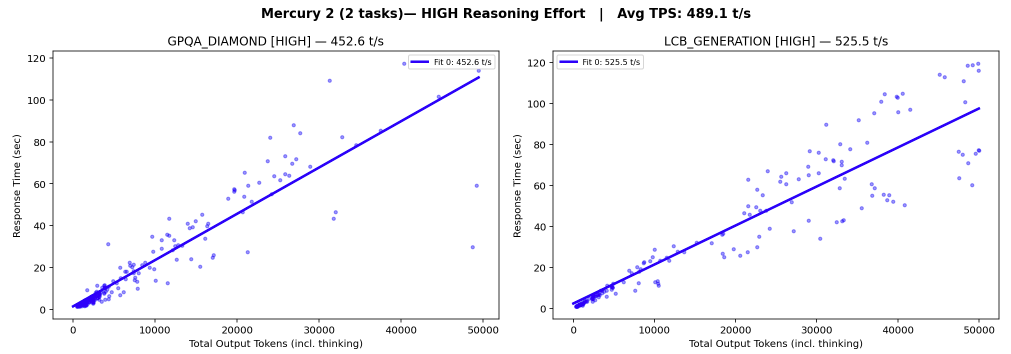
\includegraphics[width=0.9\linewidth]{assets/mercury/mercury_speed_2evals_high_grouped.png}
    \caption{\textbf{Mercury 2 token throughput (two benchmarks, \texttt{high} reasoning effort).} Including outliers where the model produces no answer tokens (i.e.,\ outputting thinking tokens only). Evaluated on GPQA Diamond and LiveCodeBench-v6; used to compute the speed reported in Figure~\ref{fig:final-pareto}. The average of per-task TPS estimates yields 489~TPS.}
    \label{fig:mercury_speed_2evals}
\end{figure}

\begin{figure}[!t]
    \centering
    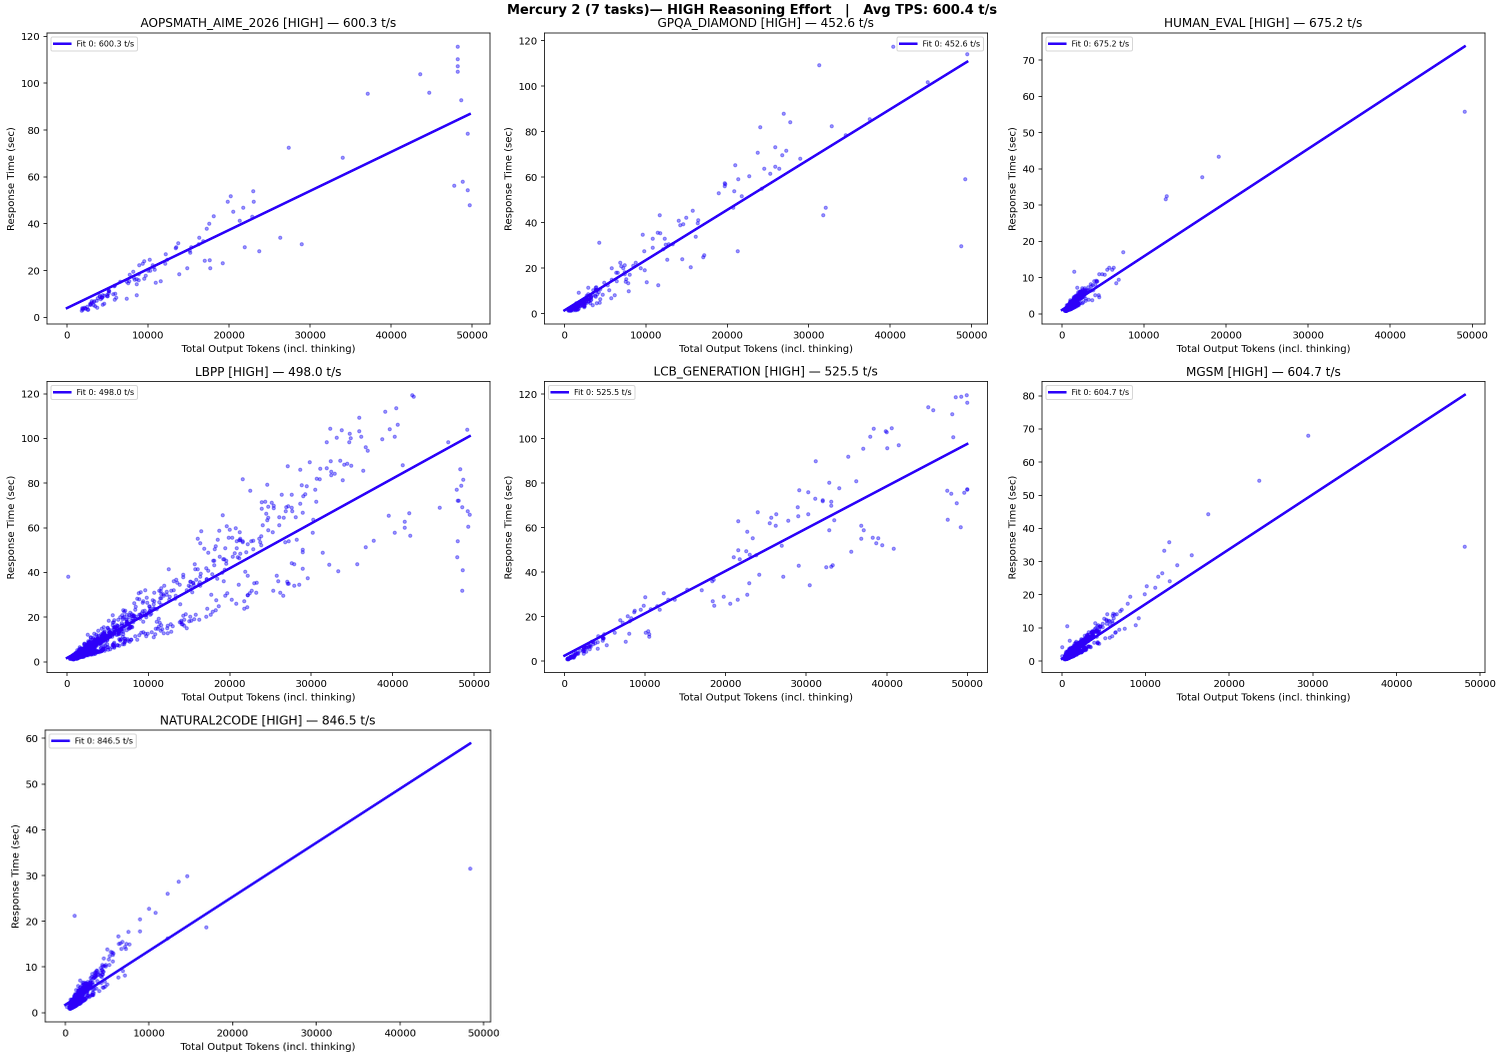
\includegraphics[width=0.9\linewidth]{assets/mercury/mercury_speed_7evals_high_grouped.png}
    \caption{\textbf{Mercury 2 token throughput (seven benchmarks, \texttt{high} reasoning effort).} Including outliers where the model produces no answer tokens (i.e.,\ outputting thinking tokens only). Used to compute the \texttt{high} effort speed reported in Table~\ref{tab:model_comparison}. Average TPS estimates yields 600~TPS.}
    \label{fig:mercury_speed_7evals_high}
\end{figure}
\begin{figure}[!t]
    \centering
    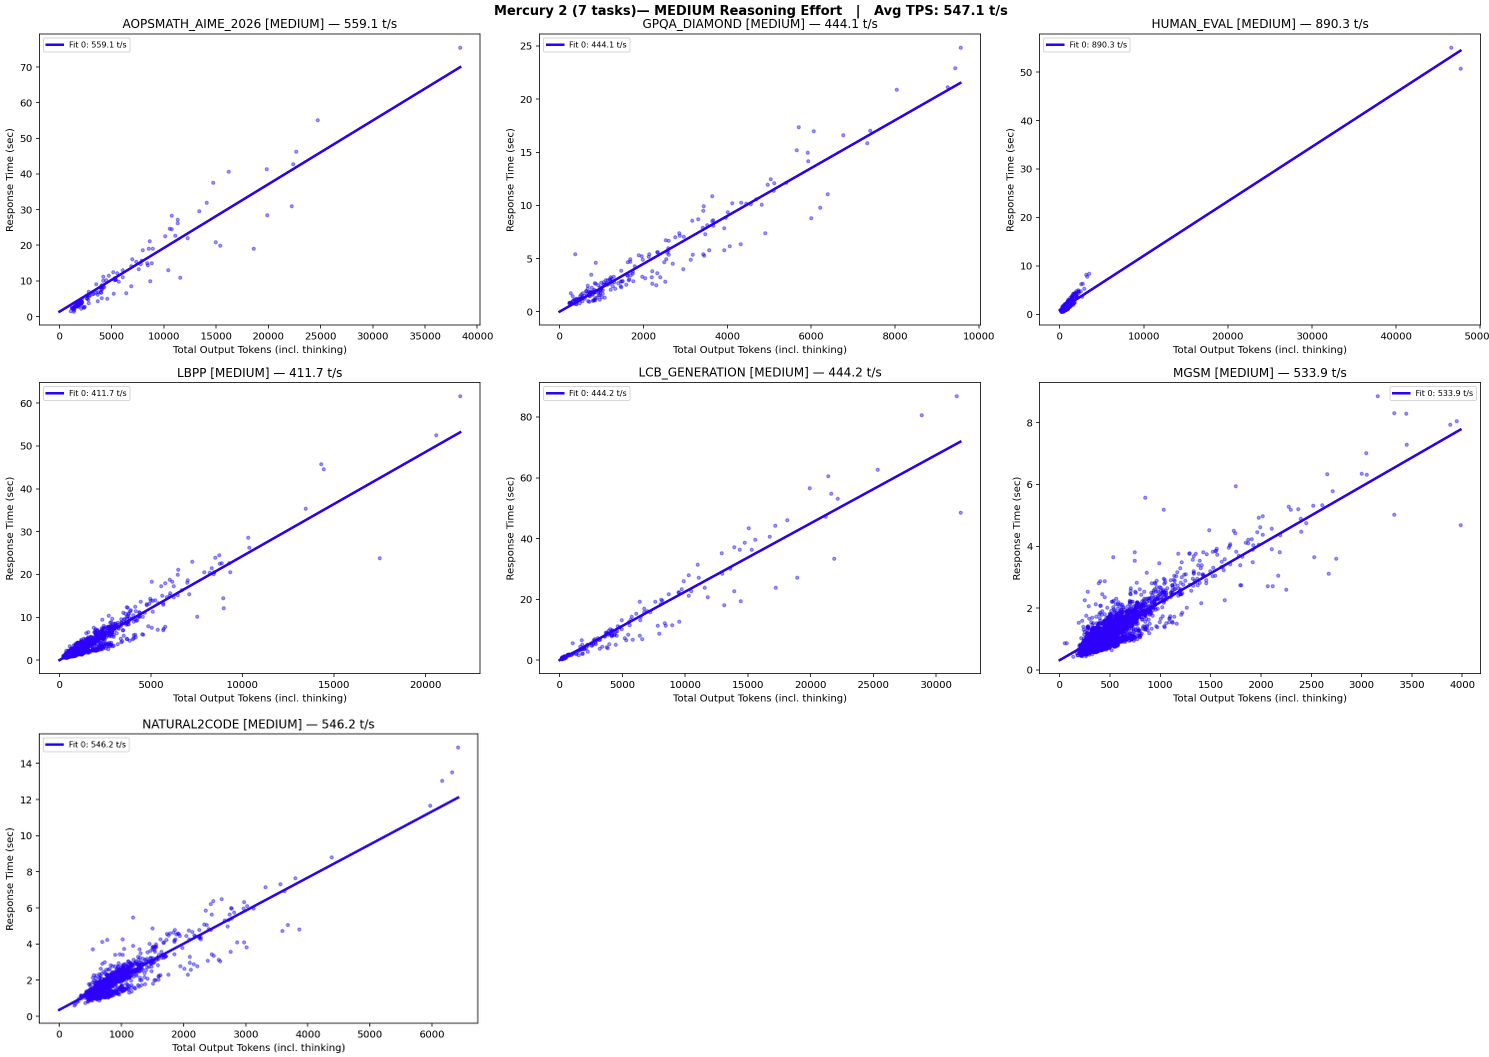
\includegraphics[width=0.9\linewidth]{assets/mercury/mercury_speed_7evals_medium_grouped.png}
    \caption{\textbf{Mercury 2 token throughput (seven benchmarks, \texttt{medium} reasoning effort).} Including outliers where the model produces no answer tokens (i.e.,\ outputting thinking tokens only). Used to compute the \texttt{medium} effort speed reported in Table~\ref{tab:model_comparison}. Average TPS estimates yields 547~TPS.}
    \label{fig:mercury_speed_7evals_medium}
\end{figure}

\newpage


\newcommand{\nothink}[1]{\textcolor{gray}{#1}}

\begin{landscape}
\section{DiffusionGemma에서 샘플링한 Denoising trajectory}
\label{appendix:denoising-trajectory}
\begin{figure}[H]
    \centering
    
\includegraphics[width=1.0\linewidth]{assets/text_diffusion_sample_3.png}
    \caption{\textbf{Example denoising trajectory sampled from DiffusionGemma}. Prompt: ``Please write a short sentence describing text diffusion.'' The color intensity denotes model confidence. The final response is ``Text diffusion is a generative process that creates high-quality text by iteratively refining random noise until a structured and coherent message emerges.'' which requires 7 denoising steps (forward passes) to generate.}
    \label{fig:text_diffusion_sample}
\end{figure}
\end{landscape}

\section{Text Diffusion의 실용적 장점 추가 설명}

\subsection{양방향 추론과 자기 수정}\label{app:advantages_bidir}

Consider the frog crossing puzzle in Figure \ref{fig:frog}. This example highlights the necessity of self-correction in logical deduction. The prompt introduces a deceptive mathematical trap---an infinite loop---that the AR baseline blindly falls into, generating a contradictory ``Yes''. DiffusionGemma's parallel generation exhibits a distinct self-correction trajectory. While it initially assigns high probability to the intuitive but incorrect ``Yes'', the bidirectional propagation of the logical constraints across the sequence enables the model to revise its stance and cleanly output ``No'' before the final tokens are sampled.


\begin{figure}[htbp]
\begin{tcolorbox}[
  colback=gray!5,
  colframe=gray!50,
  fontupper=\small,
  title={\sffamily\bfseries Prompt}
]
``A frog is trying to cross a 25-foot pond. Each hop covers exactly 5
feet and takes 1 minute. However, the lily pad located at exactly the
20-foot mark is magical: if the frog lands on it, it instantly
teleports the frog backward to the 5-foot mark. Is it possible to
reach the 25-foot pad?''

\medskip
\begin{tcolorbox}[colback=red!3, colframe=red!25, boxrule=0.4pt, left=4pt, right=4pt]
\textbf{Gemma~4 26B A4B:}
Yes, it is possible. The frog can reach the 25-foot mark by avoiding
the 20-foot mark. Since the frog's hops are exactly 5 feet, it would
land on the 5, 10, 15, 20, and 25-foot marks. To avoid the 20-foot
mark, the frog would need a different jump distance, but based on the
strict rule of ``exactly 5 feet'' per hop, it is impossible because
the frog is forced to land on the 20-foot mark to reach the 25-foot
mark.
\end{tcolorbox}

\smallskip
\begin{tcolorbox}[colback=green!3, colframe=green!30, boxrule=0.4pt, left=4pt, right=4pt]
\textbf{DiffusionGemma:}
No. To reach 25 feet, the frog must land on the 20-foot mark, which
teleports it back to 5 feet, creating an infinite loop.
\end{tcolorbox}

\smallskip
{\footnotesize \textbf{Analysis:} Gemma~4 commits to ``Yes'' without foreseeing the mathematical trap, resulting in a response that contradicts its own opening statement. DiffusionGemma converges cleanly to the correct ``No'' since the response and the reasoning can co-evolve over denoising. Note that both models are operating in non-thinking mode.}
\end{tcolorbox}

\vspace{1em}
\centering

\includegraphics[clip, viewport=0bp 0bp 500bp 230bp, width=\linewidth]{assets/frog.png}
\caption{\textbf{Denoising trace for the frog puzzle (zoomed to first 12 tokens), where color intensity indicates model confidence}. DiffusionGemma initially assigns high probability to the intuitive but incorrect ``Yes.'' After several denoising steps, bidirectional attention allows the model to realize the task is impossible and revises its initial prediction to ``No''. Denoising is completed in 6 steps.}
\label{fig:frog}
\end{figure}

\newpage
\subsection{동적이고 적응적인 계산 추가 설명}\label{app:advantages_adaptive}
To concretely demonstrate the adaptive behavior of text diffusion, we contrast a structurally ``hard'' generation task against an ``easy'' task in Figures \ref{fig:sequential} and \ref{fig:convolution}. Both tasks involve generating a sequence of binary digits governed by identical local logical rules. However, in the structurally hard variant (Figure \ref{fig:sequential}), each new token strictly depends on the two immediately preceding \emph{generated} tokens. This causal dependency requires sequential reasoning, forcing the model to resolve the logic in a predominantly left-to-right manner. Consequently, the diffusion process adaptively expends more computational effort, requiring 7 denoising steps to fully resolve the sequence. It is crucial to note, however, that even on this structurally difficult, sequential problem, DiffusionGemma successfully decodes the entire sequence of 40 tokens (20 binary digits and 20 delimiting spaces) in only 7 denoising steps---a substantial acceleration compared to the 40 discrete sequential steps an AR model would require.

Conversely, the ``easy'' convolutional variant (Figure \ref{fig:convolution}) asks the model to apply the exact same logic rules over a statically provided \emph{input} string. Because the causal dependency on the model's own dynamic output is removed, the task lacks sequential structure. DiffusionGemma immediately leverages its bidirectional attention to independently resolve all local rules in parallel, allowing the entire output sequence to converge simultaneously in merely 4 denoising steps.

\begin{figure}[htbp]
\begin{tcolorbox}[
  colback=gray!5,
  colframe=gray!50,
  fontupper=\small,
  title={\sffamily\bfseries Prompt}
]
``Generate a sequence of 20 tokens (0s and 1s) based on the following strict rules. To generate the next token, look at the two immediately preceding tokens: If the previous two tokens are 1, 1, the next token is 0. If the previous two tokens are 1, 0, the next token is 1. If the previous two tokens are 0, 1, the next token is 1. If the previous two tokens are 0, 0, the next token is 0. The starting sequence is: 0 1 Continue the sequence step-by-step until you reach exactly 20 tokens. Only emit the tokens, do not emit any other text.''

\medskip
\begin{tcolorbox}[colback=green!3, colframe=green!30, boxrule=0.4pt, left=4pt, right=4pt]
\textbf{DiffusionGemma:}
0 1 1 0 1 1 0 1 1 0 1 1 0 1 1 0 1 1 0 1
\end{tcolorbox}
\end{tcolorbox}

\vspace{1em}
\centering

\includegraphics[width=\linewidth]{assets/sequential.png}
\caption{\textbf{Denoising trace for the sequential dependency task}. Because there is a strict sequential dependency in the target output, the tokens are organically resolved in roughly a left-to-right ordering. The model adaptively allocates more compute to this ``hard'' task, taking 7 denoising steps to resolve the entire sequence of 40 tokens.}
\label{fig:sequential}
\end{figure}

\begin{figure}[htbp]
\begin{tcolorbox}[
  colback=gray!5,
  colframe=gray!50,
  fontupper=\small,
  title={\sffamily\bfseries Prompt}
]
``I will provide an input sequence of 20 binary digits. I want you to output a new sequence of the exact same length based on the following strict rules. To generate the output token at position n, look at the input sequence at position n and the input sequence at position n$-$1. If the two input tokens are 1, 1, the output token is 0. If the two input tokens are 1, 0, the output token is 1. If the two input tokens are 0, 1, the output token is 1. If the two input tokens are 0, 0, the output token is 0. For the very first token, assume the "previous" input token was a 0. Input sequence: 0 1 1 0 1 0 0 1 1 1 0 0 1 0 1 1 1 0 1 0. Only emit the tokens, do not emit any other text.''

\medskip
\begin{tcolorbox}[colback=green!3, colframe=green!30, boxrule=0.4pt, left=4pt, right=4pt]
\textbf{DiffusionGemma:}
0 1 0 1 1 1 0 1 0 0 1 0 1 1 1 0 0 1 1 1
\end{tcolorbox}

\smallskip
{\footnotesize \textbf{Analysis:} Unlike the sequential task, this prompt asks the model to apply rules over a static input string. Because the causal dependency on prior \textit{outputs} is removed, DiffusionGemma can successfully resolve all local rules in parallel.}
\end{tcolorbox}

\vspace{1em}
\centering

\includegraphics[width=\linewidth]{assets/convolution.png}
\caption{\textbf{Denoising trace for the convolutional dependency task}. Because the rules depend entirely on the statically provided input sequence rather than the model's own dynamic output, bidirectional attention allows DiffusionGemma to evaluate the ``easy'' task in parallel, only requiring 4 denoising steps to converge.}
\label{fig:convolution}
\end{figure}

\subsection{구조화되고 제약된 출력}\label{app:advantages_structure}

\begin{figure}[H]
\begin{tcolorbox}[
  colback=gray!5,
  colframe=gray!50,
  fontupper=\small\ttfamily,
  title={\normalfont\sffamily\bfseries Prompt}
]
You are a precise data extraction assistant. Your task is to extract
information from the user's text and return it strictly as a JSON
object matching the schema below. Do not include any conversational
text, explanations, or markdown formatting. Output only the raw JSON
object.

\medskip
\normalfont\small\textbf{Schema:}

{\ttfamily\small
\setlength{\parindent}{1em}

\{\\
\hspace*{1em}"type": "object",\\
\hspace*{1em}"properties": \{\\
\hspace*{2em}"first\_name": \{ "type": "string" \},\\
\hspace*{2em}"last\_name":~~\{ "type": "string" \},\\
\hspace*{2em}"age":~~~~~~~~\{ "type": "integer" \},\\
\hspace*{2em}"hobbies":~~~~\{ "type": "array",\\
\hspace*{5.5em}"items": \{ "type": "string" \} \},\\
\hspace*{2em}"is\_student": \{ "type": "boolean" \}\\
\hspace*{1em}\},\\
\hspace*{1em}"required": ["first\_name", "last\_name",\\
\hspace*{5.5em}"age", "hobbies", "is\_student"]\\
\}
}

\medskip
\normalfont\small\textbf{Input text:} ``Hi there, my name is Arthur Pendelton. I just
turned 34 last week. In my free time, I really enjoy woodworking,
baking sourdough bread, and cycling. I currently work full-time as an
accountant, having finished my master's degree five years ago.''
\end{tcolorbox}
\caption{Prompt used for the structured JSON extraction example detailed below.}
\label{fig:json-prompt}

\vspace{0.5em}

\centering
\begin{subfigure}[t]{0.48\textwidth}
  \centering
  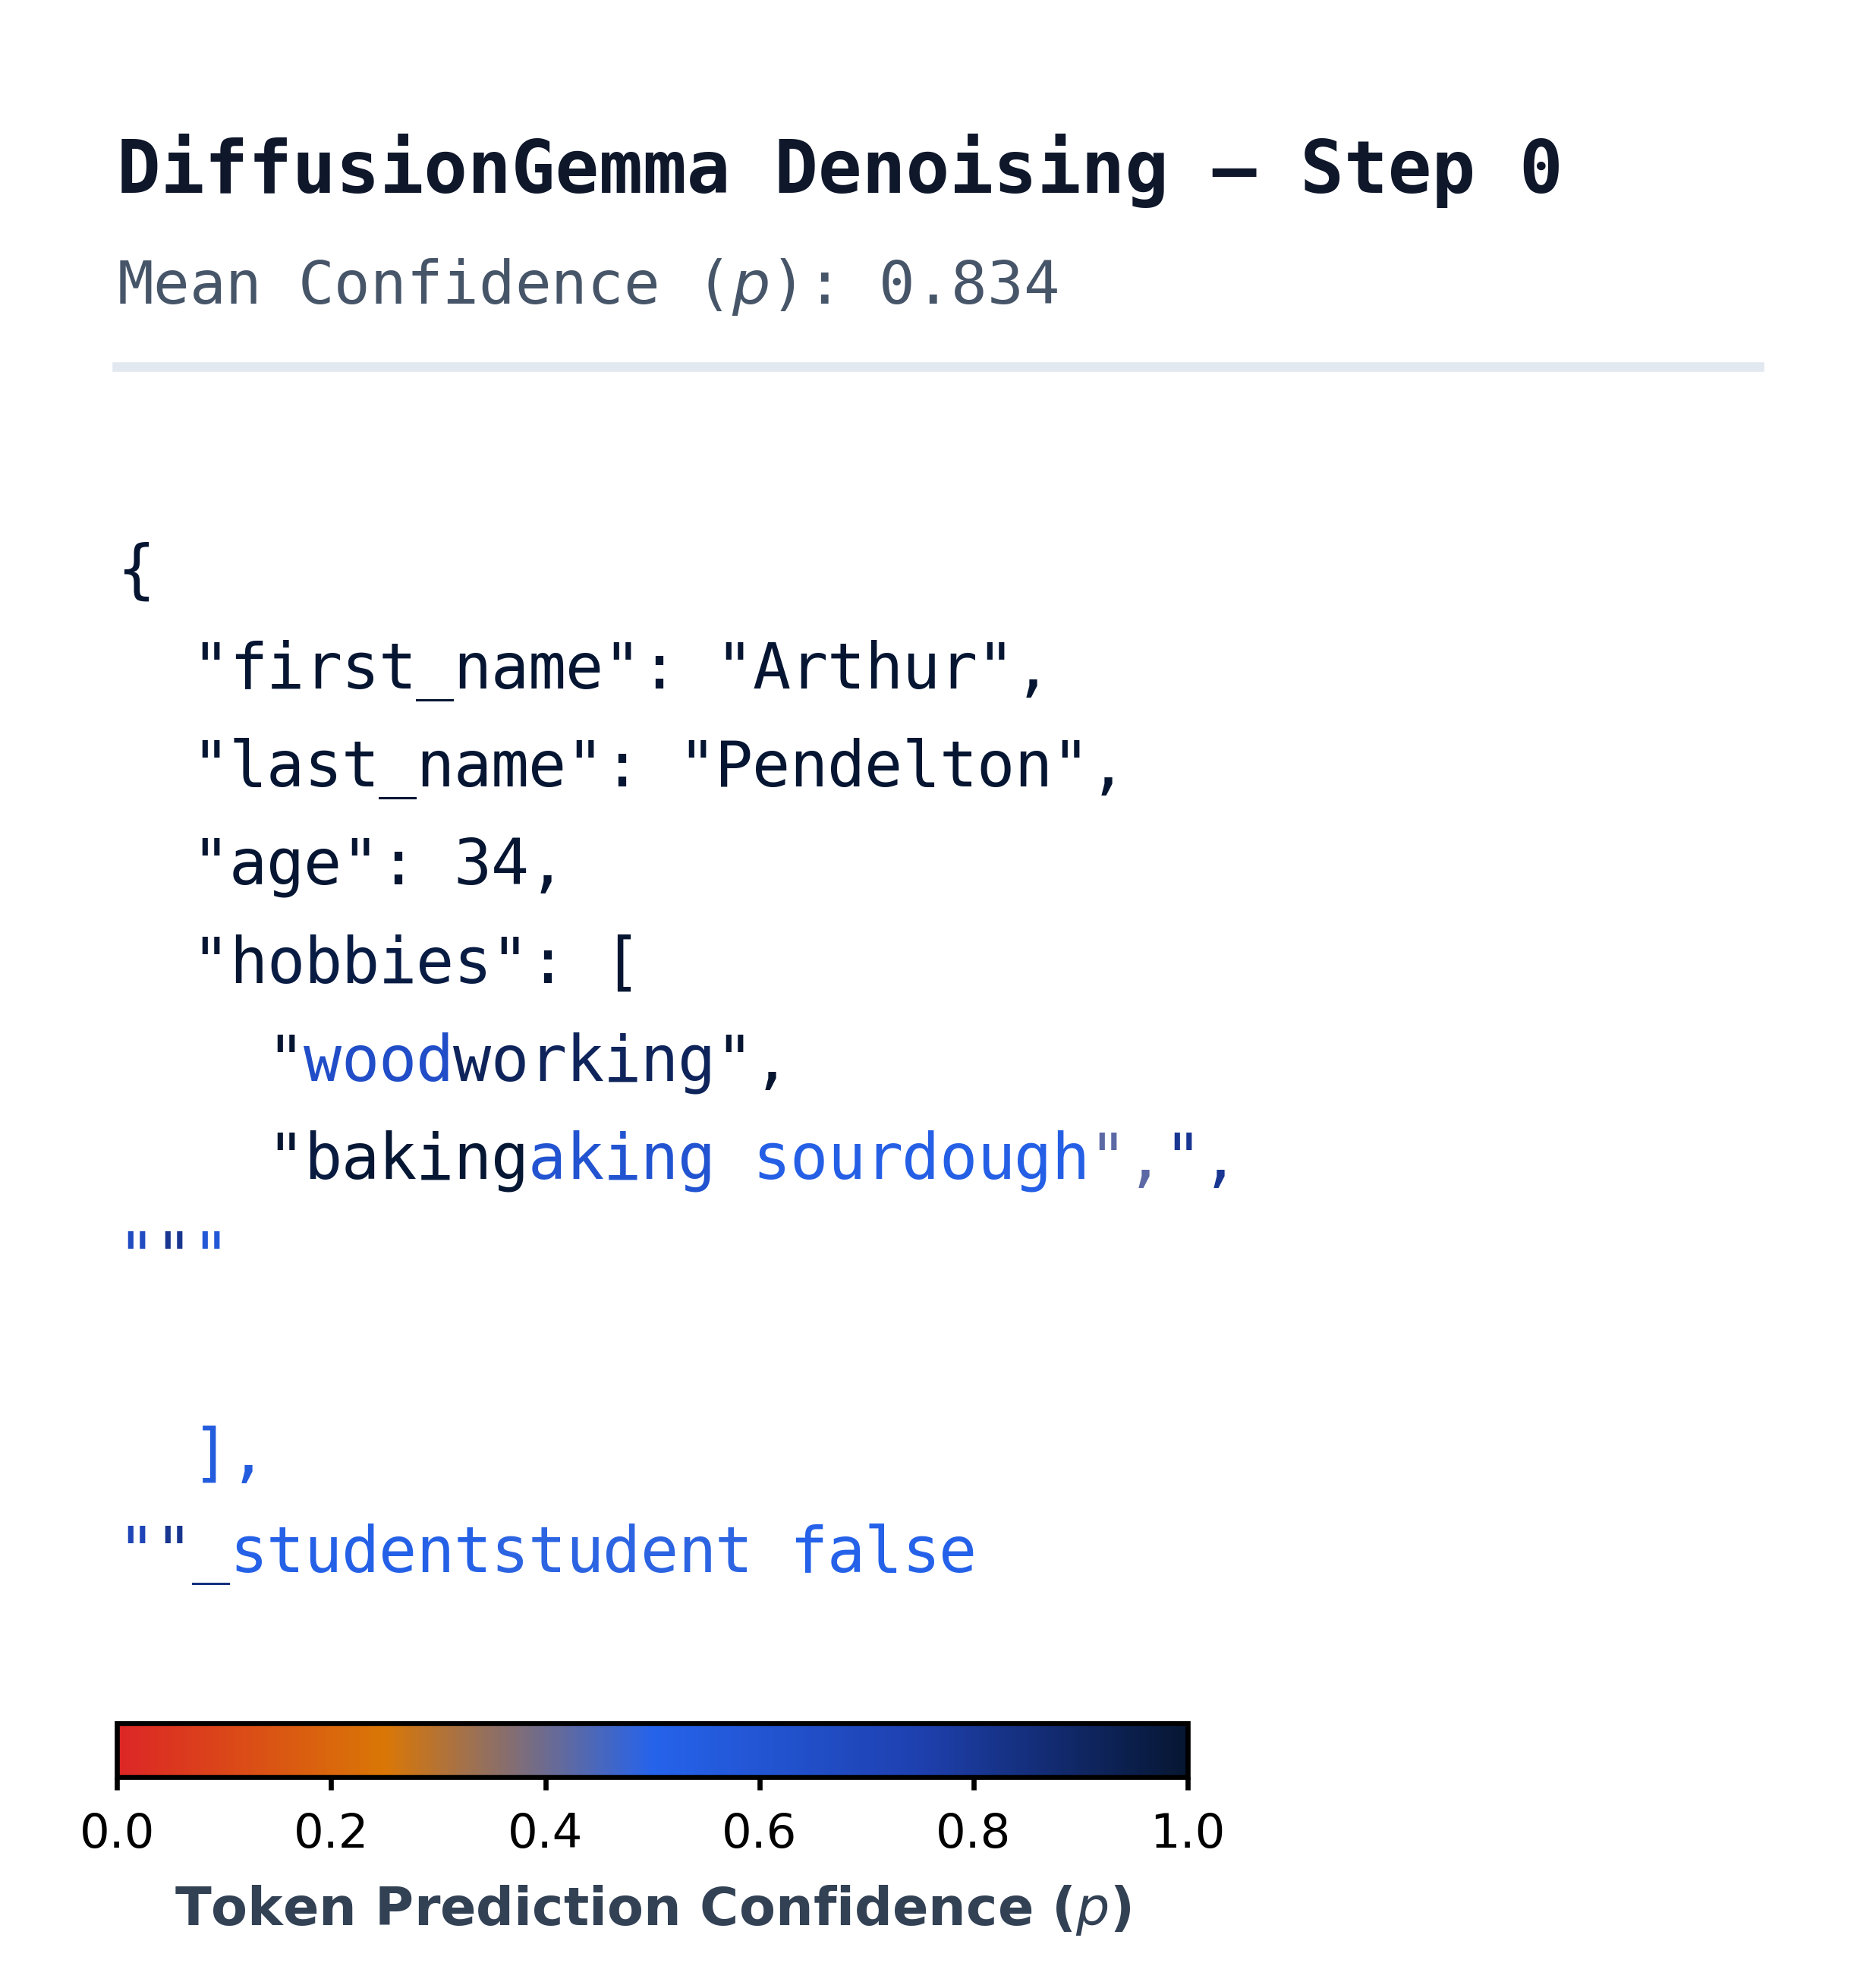
\includegraphics[width=\textwidth]{assets/td_json_canvas_0.png}
\end{subfigure}
\hfill
\begin{subfigure}[t]{0.48\textwidth}
  \centering
  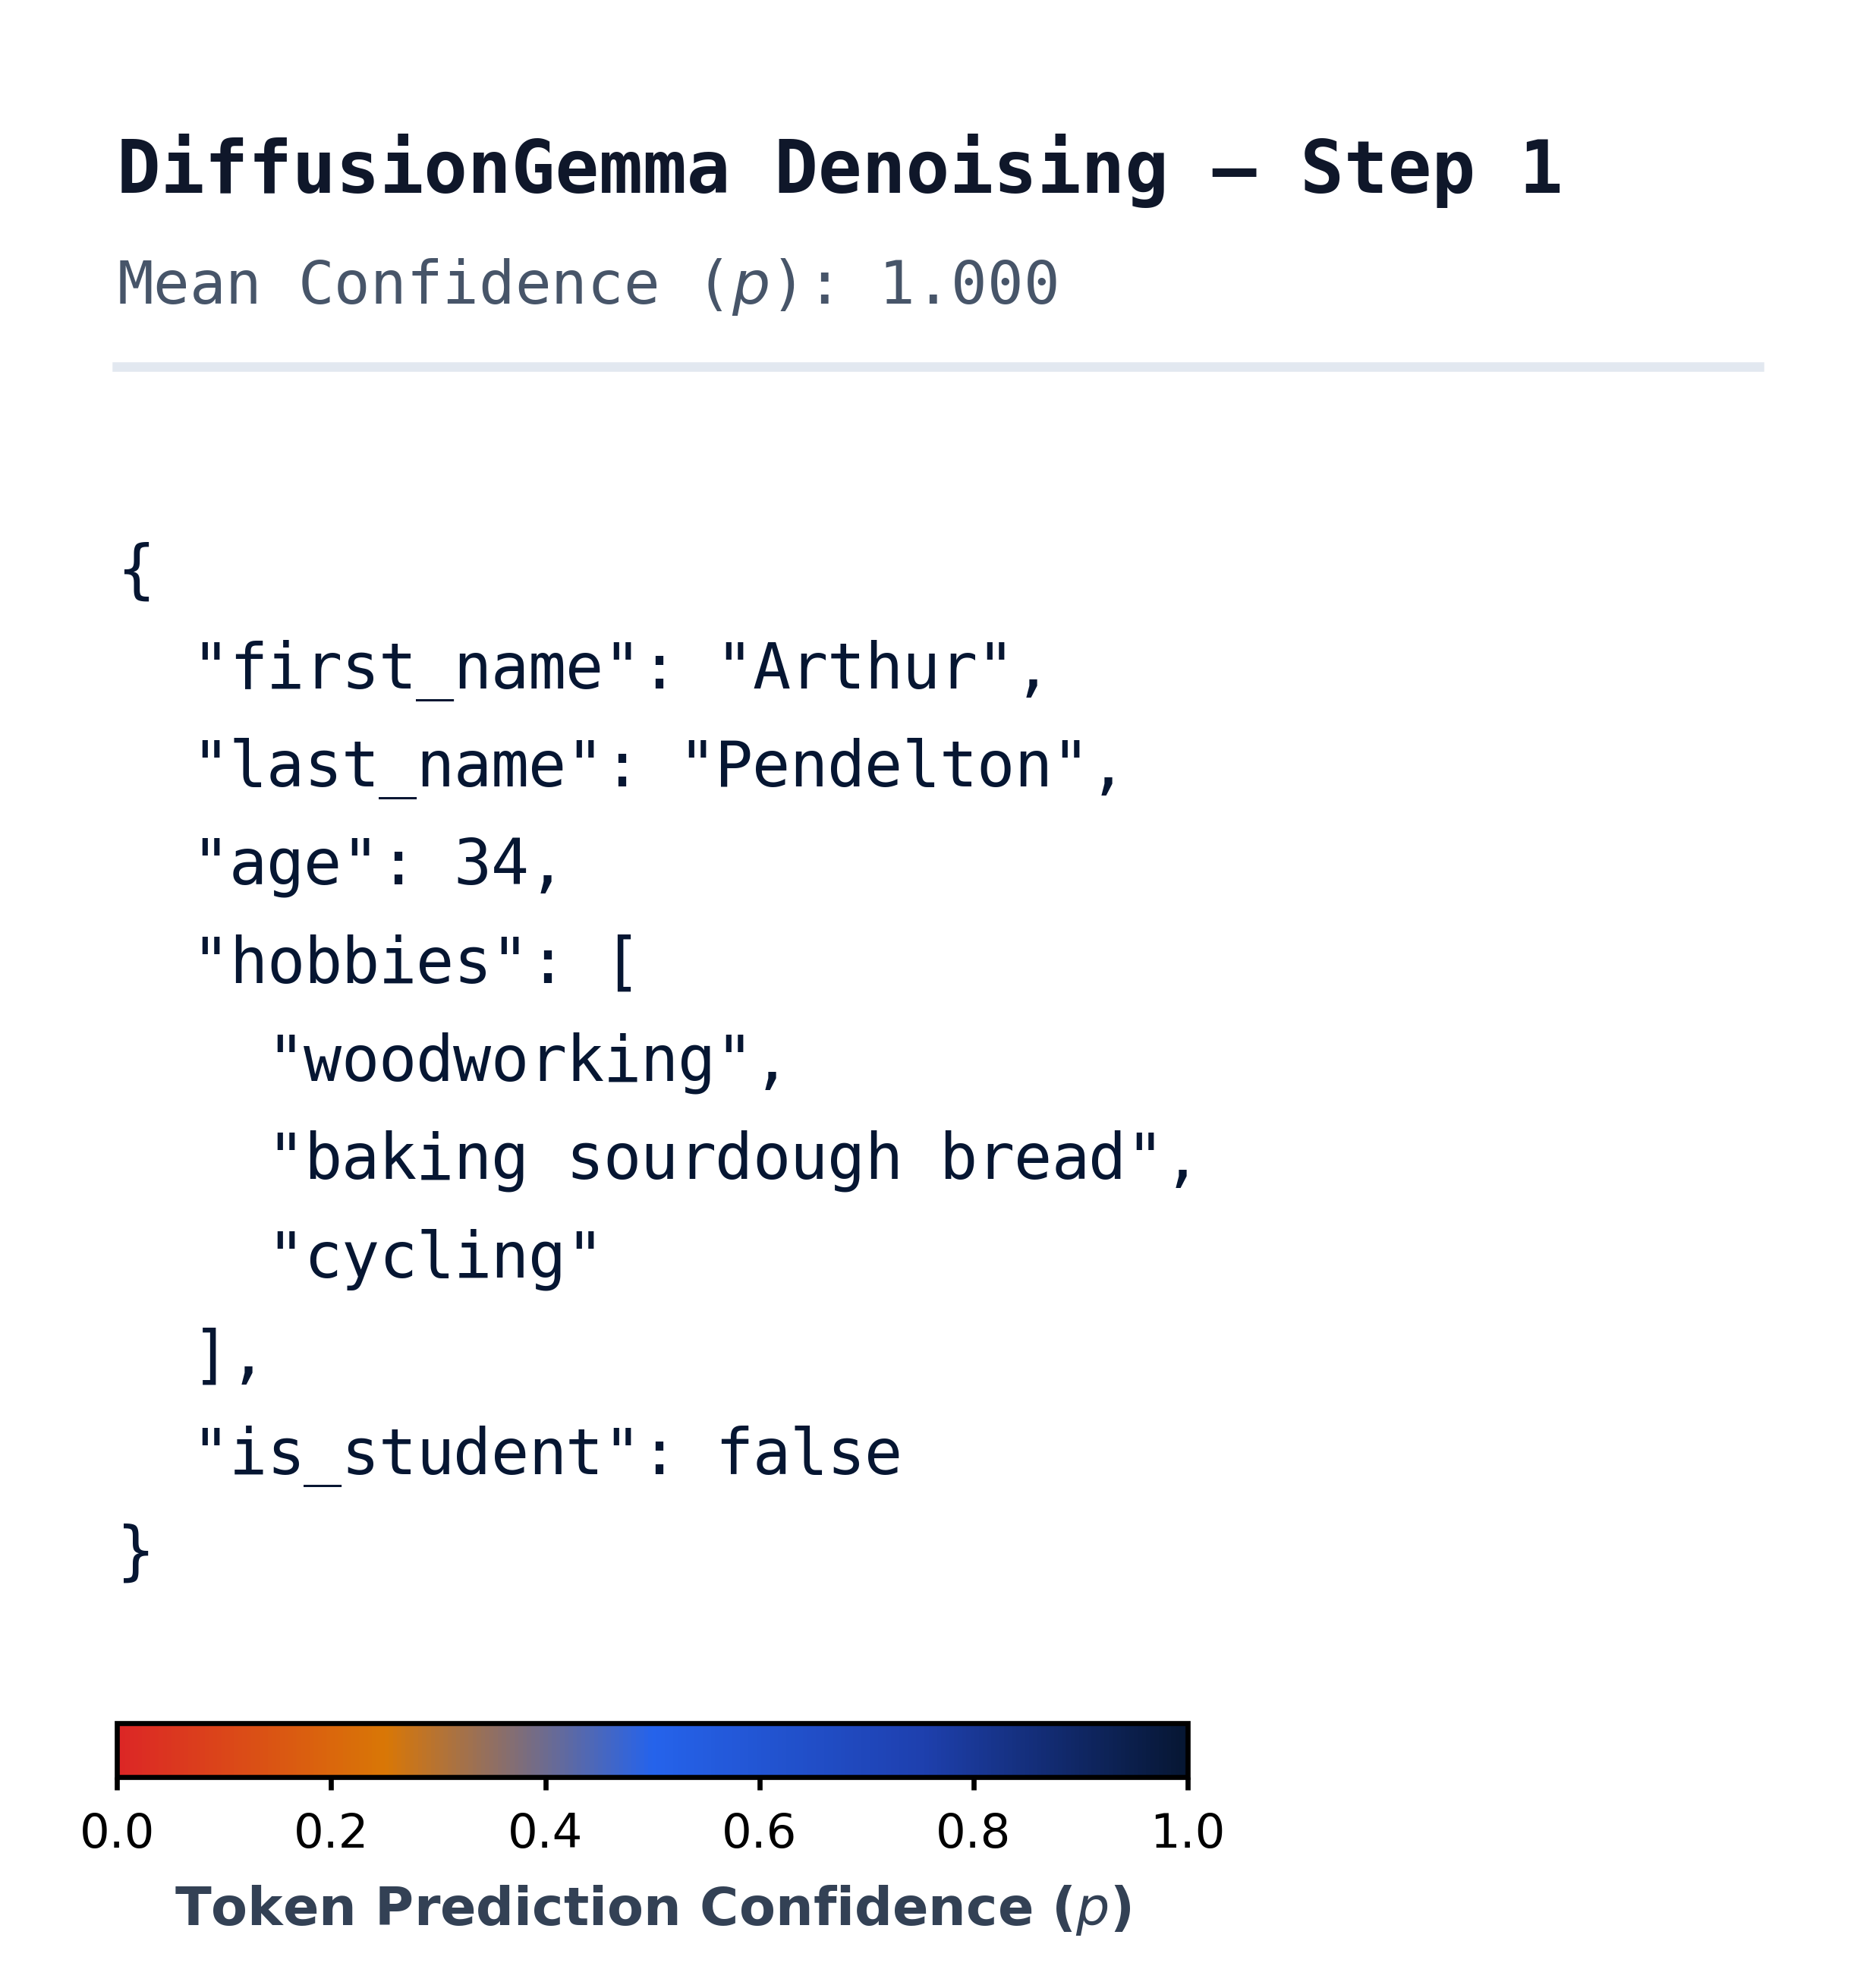
\includegraphics[width=\textwidth]{assets/td_json_canvas_1.png}
\end{subfigure}
\caption{\textbf{DiffusionGemma structured generation.} Per-token prediction confidence across denoising steps for a JSON output task. Color encodes model confidence $p$. Because the target output is heavily dictated by the provided JSON schema, text diffusion leverages parallel generation to converge almost instantaneously. The initial canvas (left) is largely correct and exhibits an average confidence exceeding 83\% per token. By the second denoising step (right), the output has fully converged to 100\% confidence, allowing the final response to be returned in just two steps.}
\label{fig:json-denoising}
\end{figure}

\begin{figure}[htbp]
\begin{tcolorbox}[
  colback=gray!5,
  colframe=gray!50,
  fontupper=\small\ttfamily,
  title={\normalfont\sffamily\bfseries Prompt}
]
Please fix this buggy python code. Output only the fixed code, nothing else:

\medskip

def get\_even\_metrics(numbers):\\
\hspace*{2em}"""Returns the total count of even numbers and a list of them."""\\
\hspace*{2em}\# Find all even numbers\\
\hspace*{2em}evens = (n for n in numbers if n \% 2 == 0)\\
\\
\hspace*{2em}\# Calculate metrics\\
\hspace*{2em}count = sum(1 for \_ in evens)\\
\hspace*{2em}even\_list = list(evens)\\
\\
\hspace*{2em}return count, even\_list
\end{tcolorbox}
\caption{Prompt used for the buggy Python code editing example.}
\label{fig:python-prompt}

\vspace{1.5em}

\centering
\begin{subfigure}[t]{0.49\textwidth}
  \vspace{0pt}
  \centering
  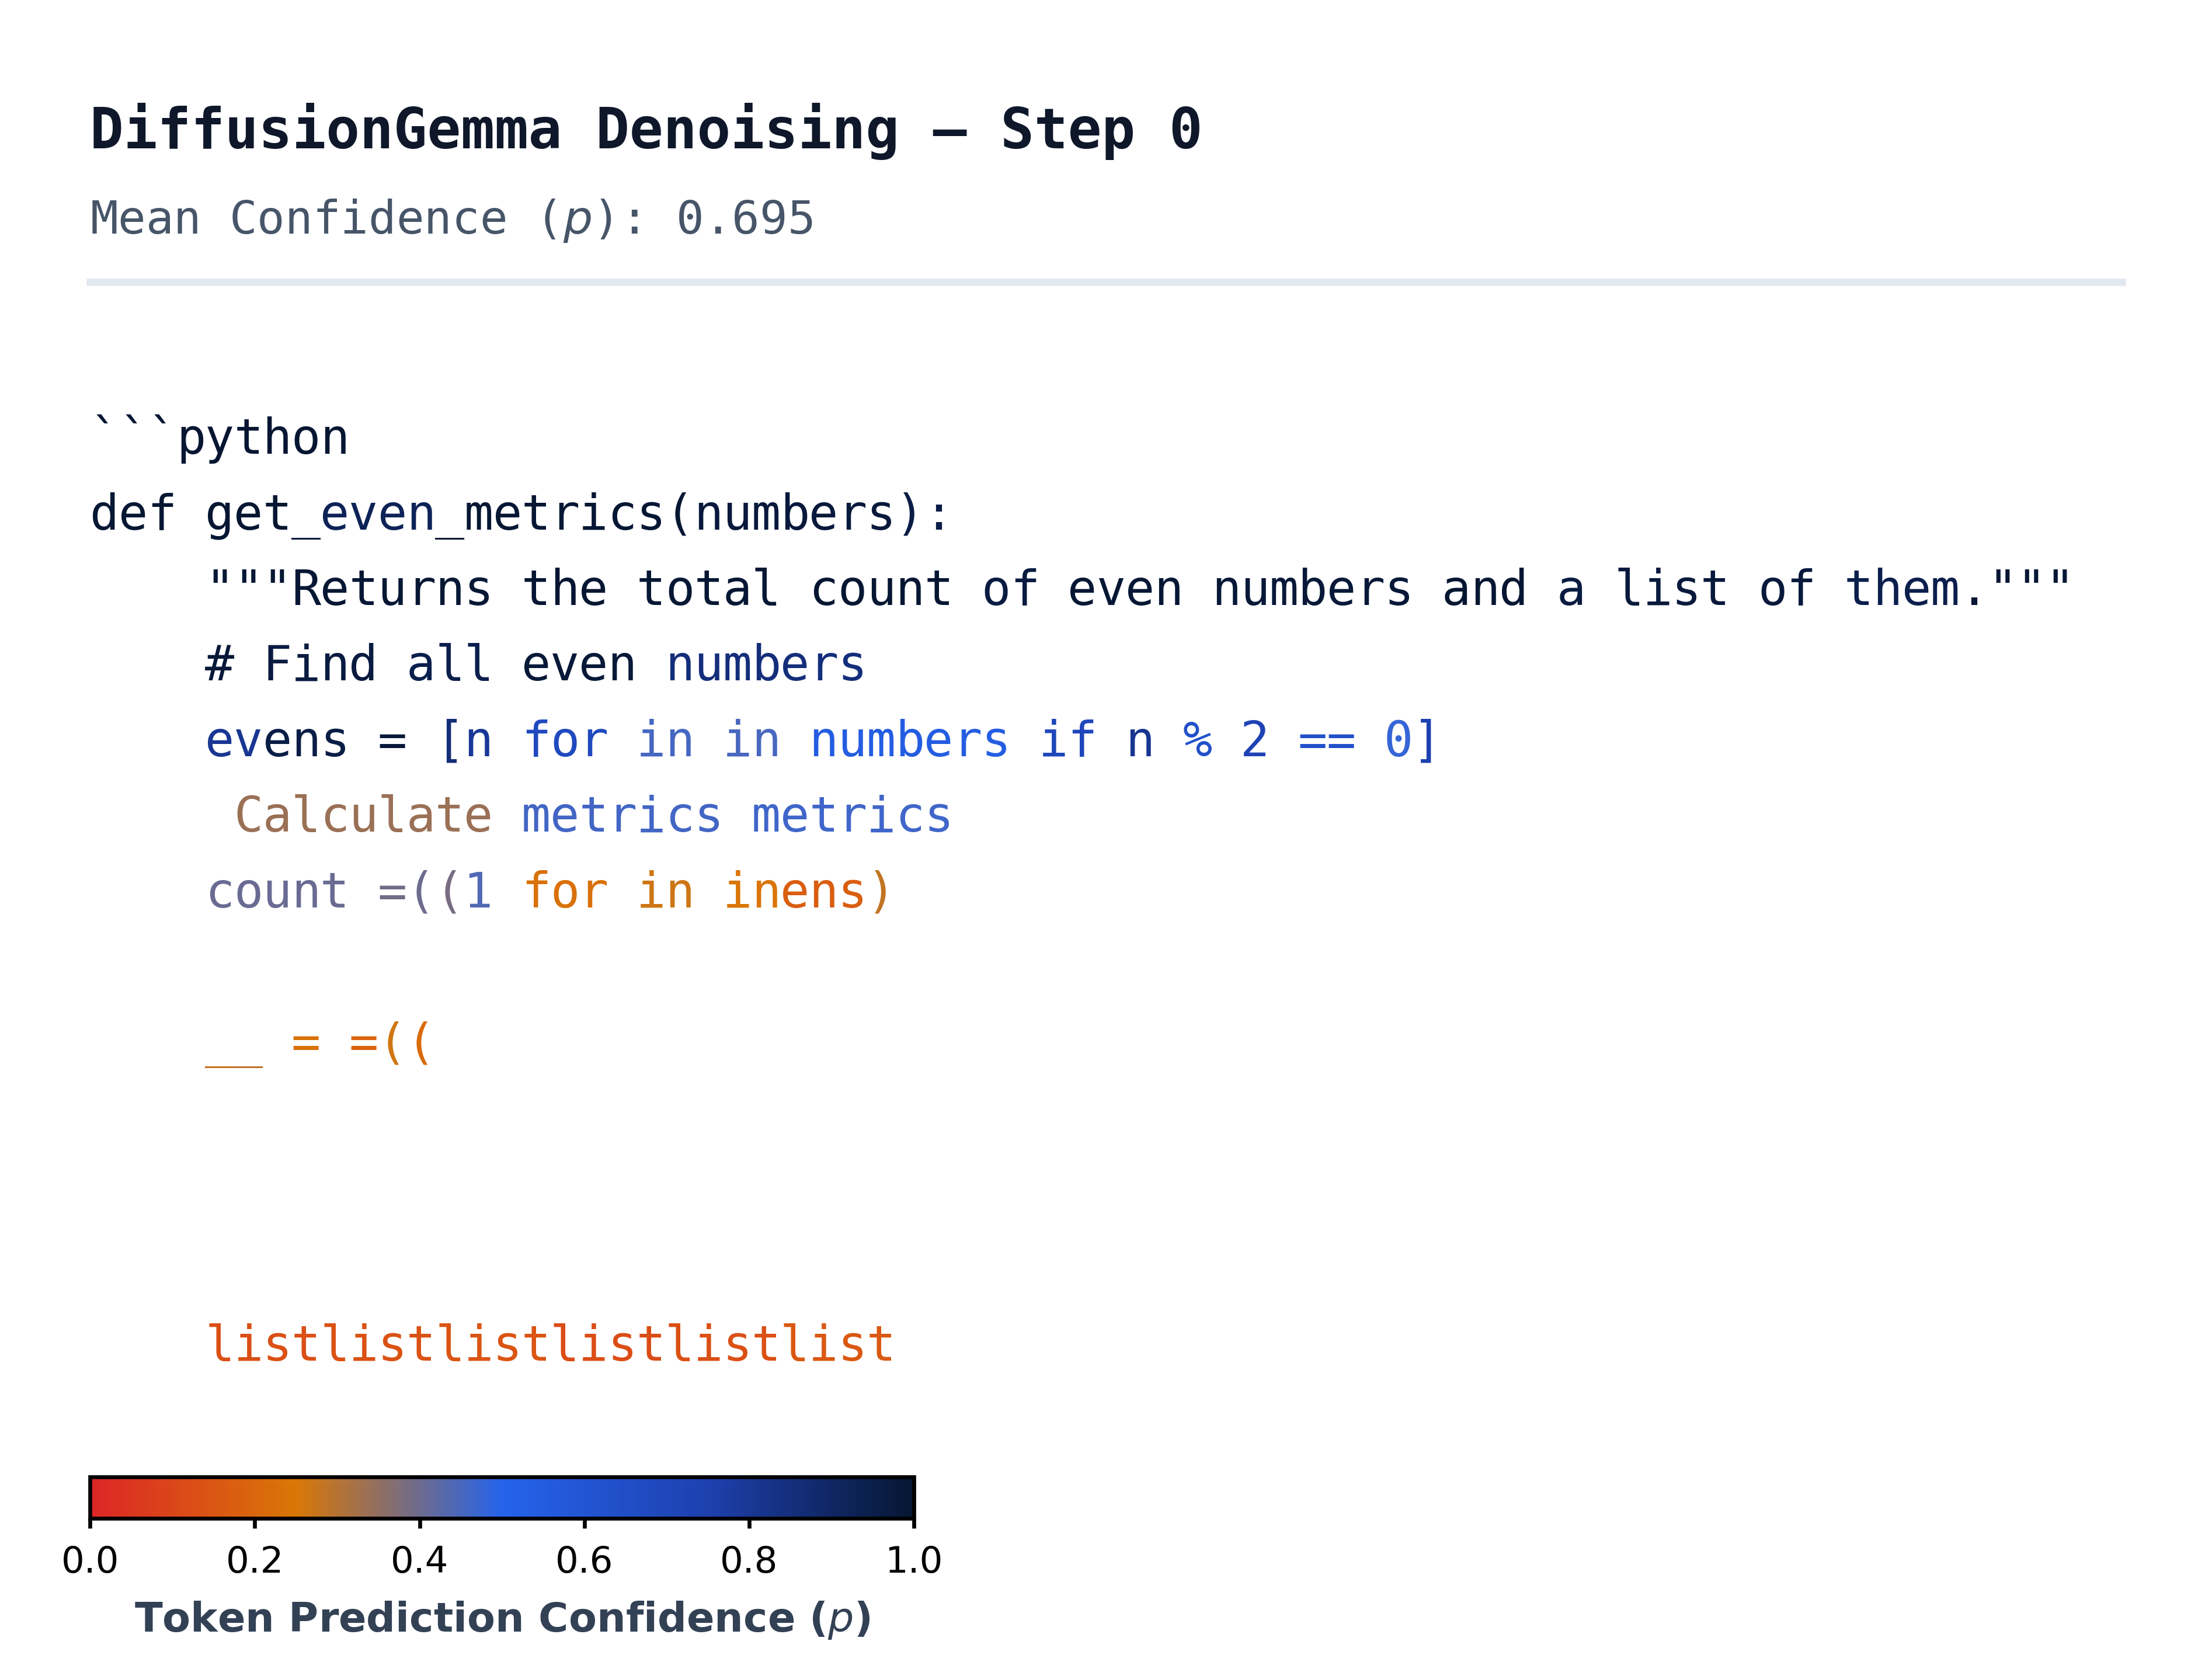
\includegraphics[width=\textwidth]{assets/td_py_0.png}
\end{subfigure}
\hfill
\begin{subfigure}[t]{0.49\textwidth}
  \vspace{0pt}
  \centering
  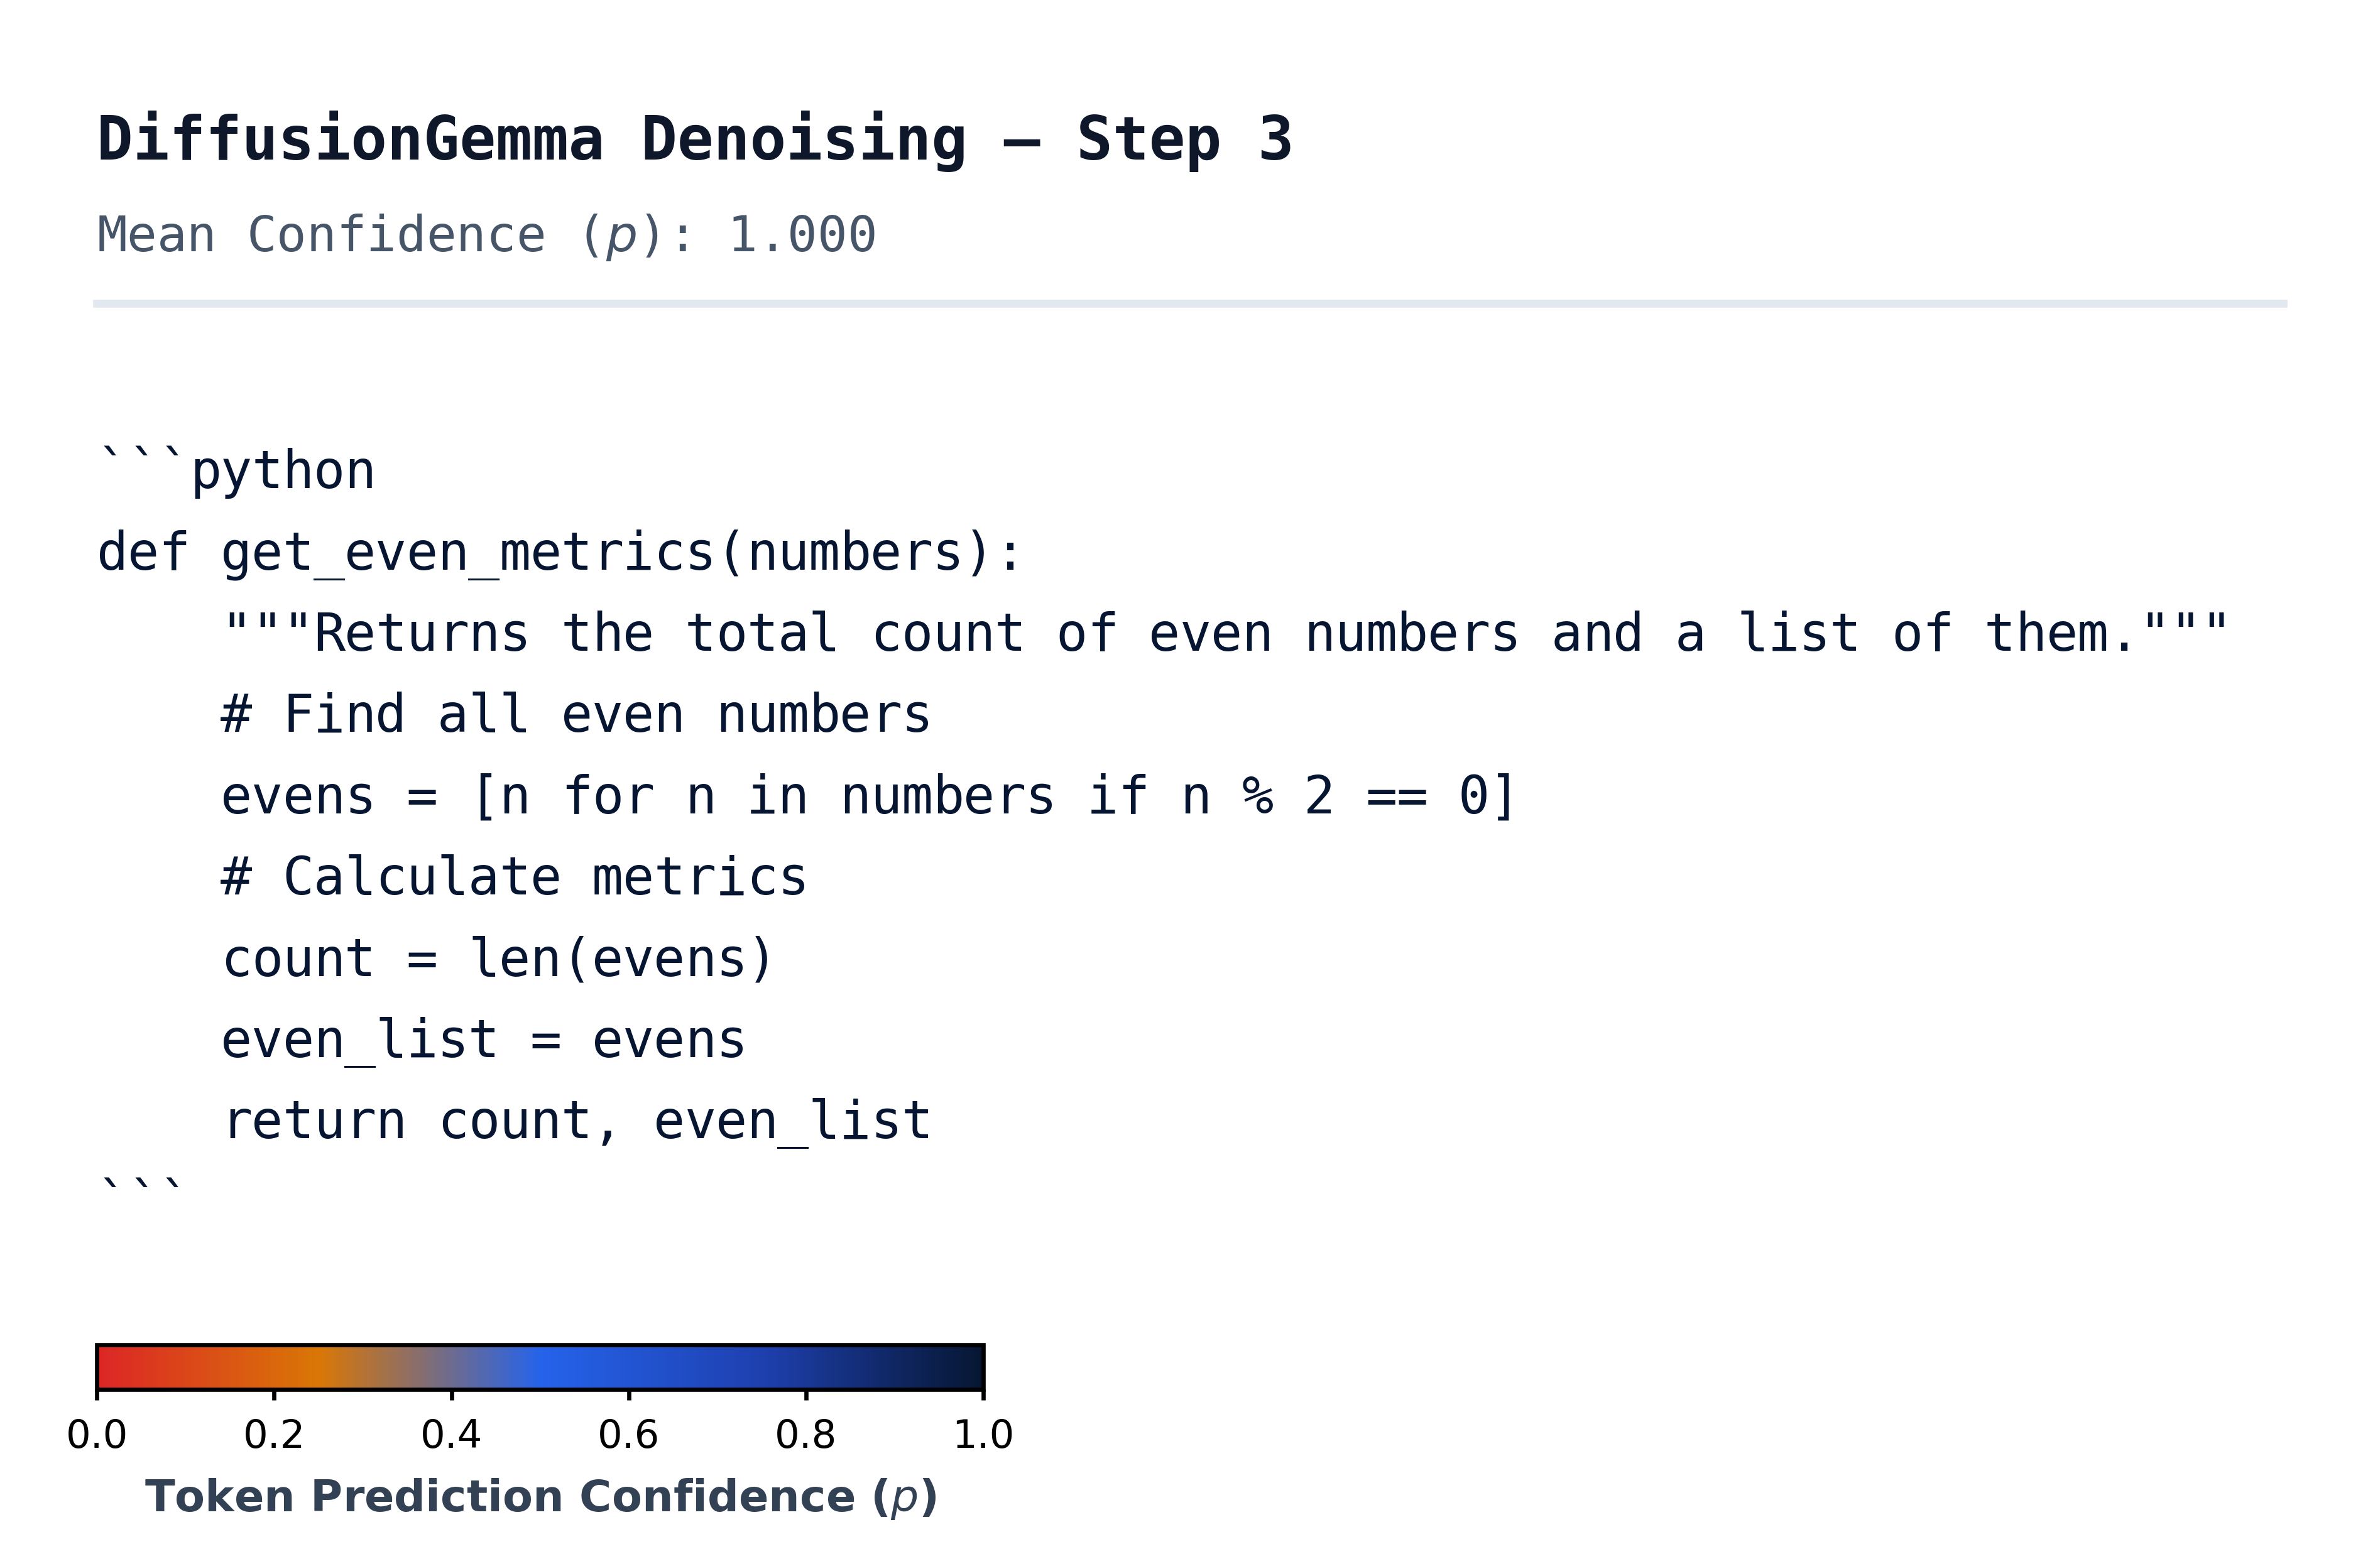
\includegraphics[width=\textwidth]{assets/td_py_3.png}
\end{subfigure}
\caption{\textbf{DiffusionGemma code editing.} Per-token prediction confidence across denoising steps for a code debugging task. Color encodes model confidence $p$. Because the output space is strictly constrained by the input---the vast majority of tokens are copied verbatim, and only a localized semantic fix is required---the diffusion process converges rapidly. The corrected, bug-free implementation is generated in just three denoising steps.}
\label{fig:bug-fix}
\end{figure}

\end{document}
